\documentclass[11pt]{article}

\usepackage[top=0.9in,bottom=1.0in,left=1.0in,right=1.0in]{geometry}
\usepackage{amsmath,amssymb,amsthm}
\usepackage{graphicx}
\usepackage{booktabs}
\usepackage{enumitem}
\usepackage{xcolor}
\usepackage{listings}
\usepackage[colorlinks=true,linkcolor=blue!60!black,urlcolor=blue!60!black]{hyperref}
\usepackage{titlesec}
\usepackage{parskip}

\titlespacing*{\section}{0pt}{14pt}{6pt}
\titlespacing*{\subsection}{0pt}{10pt}{4pt}

\theoremstyle{definition}
\newtheorem{theorem}{Theorem}[section]
\newtheorem{lemma}[theorem]{Lemma}
\newtheorem{corollary}[theorem]{Corollary}
\newtheorem{definition}[theorem]{Definition}

\theoremstyle{remark}
\newtheorem*{gotcha}{Gotcha}
\newtheorem*{observation}{Empirical observation}

\lstset{
  basicstyle=\ttfamily\small,
  breaklines=true,
  frame=single,
  framesep=4pt,
  backgroundcolor=\color{gray!8},
  columns=fullflexible,
  keepspaces=true
}

\newcommand{\Sw}{S_W}
\newcommand{\Sb}{S_B}
\newcommand{\St}{S_T}
\newcommand{\R}{\mathbb{R}}
\newcommand{\tr}{\operatorname{tr}}
\newcommand{\rank}{\operatorname{rank}}

\title{\textbf{Eigenfaces vs.\ Fisherfaces}\\[4pt]
\large A study guide with full derivations, code notes and measured results}
\author{Shubh Karman Singh (26M0843) \and Saumya Bajpai (26D0366)}
\date{CS 740 Project \\ \today}

\begin{document}
\maketitle

\begin{abstract}
\noindent
This guide covers the paper P.~N.~Belhumeur, J.~P.~Hespanha and D.~J.~Kriegman,
\emph{``Eigenfaces vs.\ Fisherfaces: Recognition Using Class Specific Linear
Projection''}, IEEE TPAMI 19(7), 1997. It is written to be read from a standing
start: every derivation is done line by line, and every claim about the code is
tied to a number actually produced by our MATLAB script
\texttt{fisherfaces\_project.m}. Every experimental figure quoted here comes from
\texttt{run\_log.txt} in the same directory.
\end{abstract}

\tableofcontents

\section{Notation used everywhere in this document}

One image is turned into one long column vector by stacking its pixels. Everything
below uses the symbols in Table~\ref{tab:notation}, and no symbol ever changes
meaning.

\begin{table}[htbp]
\centering
\small
\begin{tabular}{cll}
\toprule
Symbol & Meaning & Value / note \\
\midrule
\multicolumn{3}{l}{\emph{PCA --- the notation used in the course slides and HW3 Q1}}\\
$d$                & number of pixels in one image            & ORL $10304$, Yale $32256$ \\
$N$                & number of training images                & ORL $192$, Yale $1520$ \\
$x_i$              & the $i$th training image, in $\R^d$      & $i = 1,\dots,N$ \\
$\bar{x}$          & mean of the training images (mean face)  & $\bar{x}=\tfrac1N\sum_i x_i$ \\
$\bar{x}_i$        & the $i$th mean-deducted image            & $\bar{x}_i = x_i - \bar{x}$ \\
$X$                & $[\,\bar{x}_1|\cdots|\bar{x}_N\,]$       & $d\times N$ \\
$C$                & covariance matrix, $C \propto XX^{\!\top}$ & $d\times d$ \\
$S$                & scatter matrix $\sum_i \bar{x}_i\bar{x}_i^{\!\top} = XX^{\!\top}$ & $S=(N-1)C$ \\
$L$                & the small matrix $X^{\!\top}\!X$          & $N\times N$ \\
$w$                & an eigenvector of $L$                    & $w\in\R^N$ \\
$V$                & eigenvector matrix of $C$, $CV=V\Lambda$ & $d\times d$, $V^{\!\top}V=I$ \\
$V_l$              & the $l$th eigenvector (an eigenface)     & $V_l\in\R^d$ \\
$\hat{V}_k$        & the eigenspace $V(:,1{:}k)$              & $d\times k$ \\
$\Lambda,\lambda_l$ & eigenvalues, $\lambda_1\ge\cdots\ge\lambda_d\ge 0$ & \\
$\alpha_{il}$      & $l$th eigen-coefficient of $x_i$         & $\alpha_{il}=V_l^{\!\top}\bar{x}_i$ \\
$\tilde{x}_i$      & rank-$k$ approximation to $x_i$          & \\
$u$, $J(u)$        & a candidate direction, and its total reconstruction error & \\
$k$                & number of eigenfaces kept                & swept $1\ldots170$ \\
\midrule
\multicolumn{3}{l}{\emph{LDA --- additional symbols (Duda, Hart \& Stork)}}\\
$c$                & number of classes (people)               & ORL $32$ or $40$, Yale $38$ \\
$j$                & class index                              & $j = 1,\dots,c$ \\
$n_j$              & training images of person $j$            & ORL $6$, Yale $40$ \\
$\mu_j$            & mean of the images of class $j$          & \\
$\St,\Sb,\Sw$      & total, between-class, within-class scatter & \\
$m$                & PCA dimensions kept \emph{before} LDA    & paper uses $N-c$ \\
$w_l$, $W$         & the $l$th Fisherface, and their matrix   & $d\times(c-1)$ \\
\bottomrule
\end{tabular}
\caption{Notation. The PCA block follows the course slides (``PCA: algorithm'',
slides 98--113) and the HW3 problem sheet, so this guide can be read side by side
with them.}
\label{tab:notation}
\end{table}

\paragraph{A note on symbols.} Three indices are used and never swap roles: $i$
runs over \textbf{training images}, $l$ over \textbf{components} (eigenfaces or
Fisherfaces), and $j$ over \textbf{classes}.

Two cautions, both of which come from following the sources faithfully.
\emph{First}, the letter $w$ does double duty: in Part~I it is an eigenvector of
the small matrix $L=X^{\!\top}\!X$ and lives in $\R^N$ (slide 113), while in
Parts~II--III it is a Fisher discriminant direction in $\R^d$. They never appear
in the same derivation, and the dimension tells them apart.
\emph{Second}, the slides define the covariance with the unbiased denominator,
$C=\frac{1}{N-1}\sum_i \bar{x}_i\bar{x}_i^{\!\top}$, whereas the HW3 solution to
Q1(i) --- and our code --- use $\frac{1}{N}$. The eigen\emph{vectors} are
identical either way; only the eigenvalues differ by the factor
$\tfrac{N-1}{N}$. We use $\frac{1}{N}$ throughout so that the reconstruction-error
identity of Theorem~\ref{thm:recon} reads exactly as it does in the HW3 solution,
and we flag the difference wherever eigenvalues are quoted numerically.

\medskip
\noindent\emph{The code uses the same names.} The MATLAB script deliberately
mirrors this notation: \texttt{xbar} is $\bar{x}$, \texttt{X} is the
mean-deducted data matrix, \texttt{L} is $X^{\!\top}\!X$, \texttt{W} (inside
\texttt{doPCA}) holds the eigenvectors $w$ of $L$, \texttt{V} is the eigenface
matrix and \texttt{Vk}/\texttt{Vm} a truncated eigenspace $\hat{V}_k$, and
\texttt{Alpha} holds the eigen-coefficients $\alpha_{il}$. Raw (not yet centred)
image matrices are named \texttt{imgs}, \texttt{imTr}, \texttt{imTe}, since
$X$ is reserved for the centred data.

\paragraph{Why stacking pixels into a vector is allowed.}
A $112\times 92$ image has $10304$ numbers in it. Writing them as a $10304$-long
column simply chooses an order for those numbers. Every method here (PCA, LDA,
nearest neighbour) only ever uses sums, differences and inner products of whole
images, and all of those are unchanged by reordering the entries, as long as we use
the \emph{same} order for every image. We lose the knowledge that pixel $(5,7)$ is
next to pixel $(5,8)$ -- these methods genuinely do not know the image is 2-D --
but nothing becomes incorrect.

\medskip
In MATLAB the stacking is \texttt{im(:)}, which reads the matrix \textbf{column by
column} (``column-major'' order). The inverse is
\texttt{reshape(v, height, width)}. The two must always be used as a matched pair;
reshaping with the width and height swapped gives a scrambled image.

\section{The two databases}

\begin{table}[htbp]
\centering
\small
\begin{tabular}{lll}
\toprule
 & \textbf{ORL (AT\&T)} & \textbf{Cropped Extended Yale B} \\
\midrule
Image size        & $92\times112 = 10304$ px & $168\times192 = 32256$ px \\
Subjects          & $40$                     & $38$ (\texttt{yaleB14} absent) \\
Images per subject& exactly $10$             & $59$--$64$, \emph{not} constant \\
Total images      & $400$                    & $2414$ \\
Pose              & varies (tilt, rotation)  & \textbf{fixed} --- every file is \texttt{P00} \\
Expression        & varies                   & fixed \\
Glasses           & varies                   & fixed \\
Lighting          & essentially constant     & \textbf{the only thing that varies} \\
\bottomrule
\end{tabular}
\caption{The two databases are near-complements: ORL varies everything
\emph{except} lighting, Yale varies \emph{only} lighting. That is what makes the
pair a controlled experiment rather than two arbitrary datasets.}
\label{tab:datasets}
\end{table}

Yale encodes the lamp position in the filename as
\texttt{A$\pm$azimuth\,E$\pm$elevation}: azimuth spans $-130^\circ$ to $+130^\circ$
(29 distinct values) and elevation $-40^\circ$ to $+90^\circ$ (12 values). Binned
by angle from the optical axis into the paper's standard subsets, subject 1's 64
images split as $7$ at $\le12^\circ$, $12$ at $\le25^\circ$, $10$ at $\le50^\circ$,
$16$ at $\le77^\circ$ and $\mathbf{19}$ beyond $77^\circ$. Nearly a third of the
database is lit from more than $77^\circ$ off-axis, which is why some frames in
Figure~\ref{fig:datasets} are almost entirely black.

\begin{figure}[htbp]
\centering
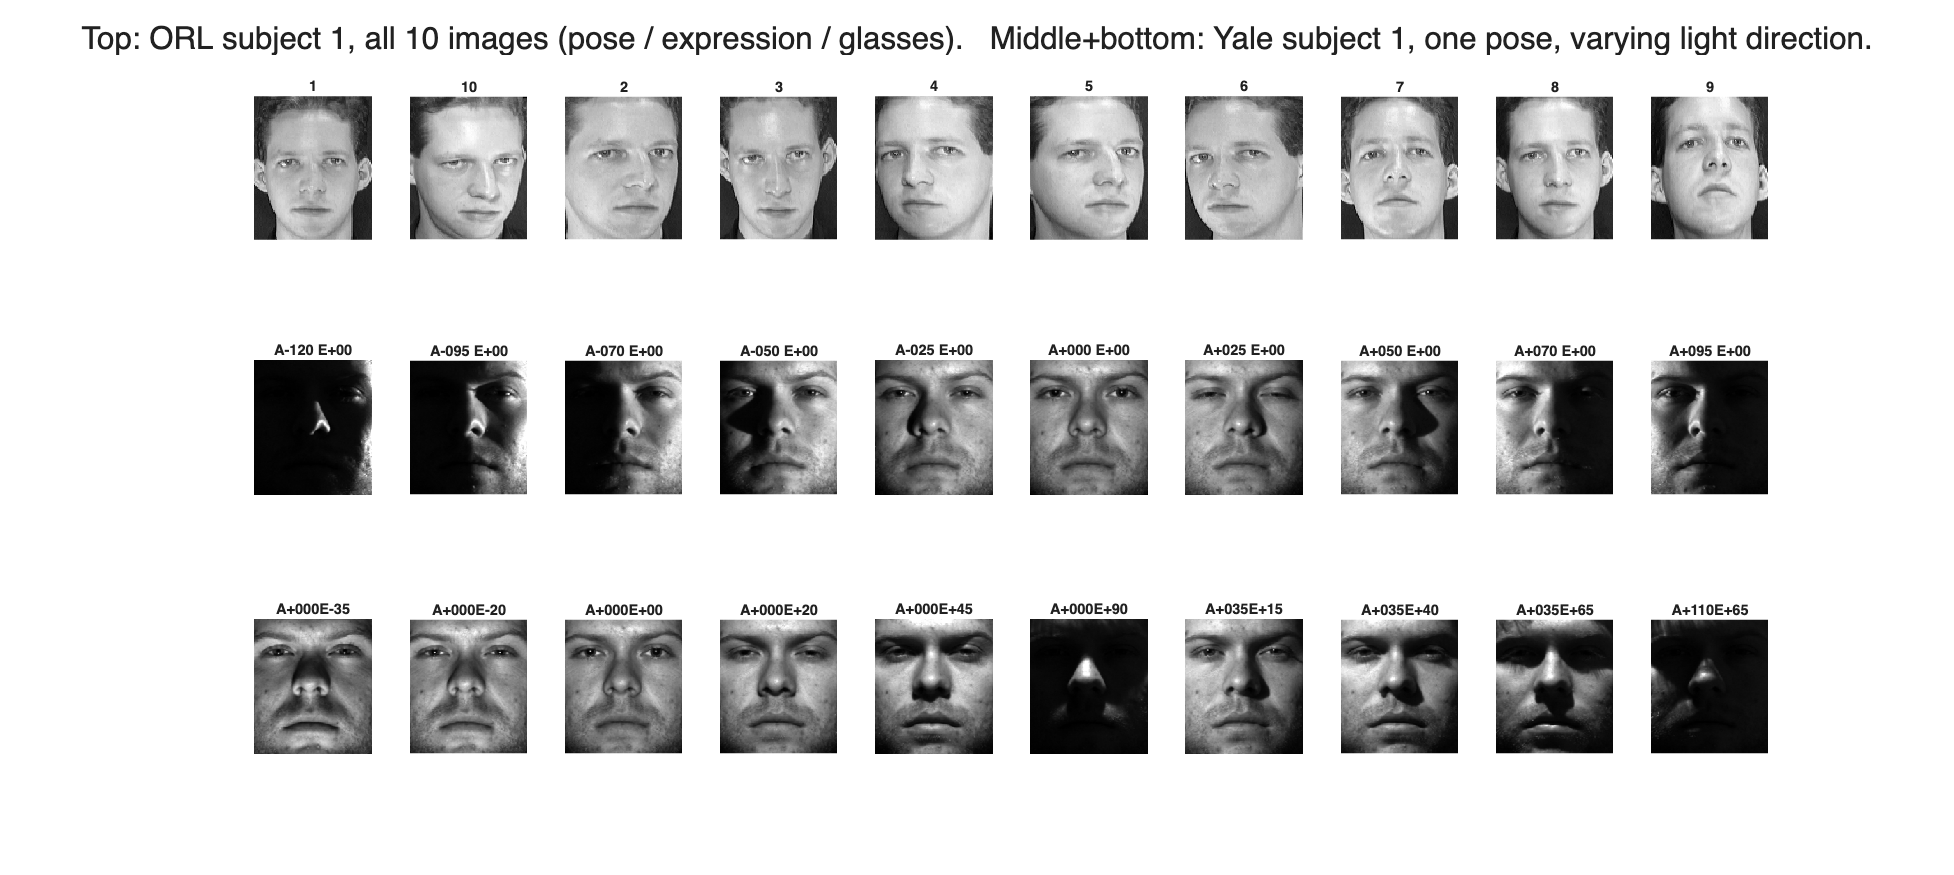
\includegraphics[width=\textwidth]{figs/s0_datasets.png}
\caption{Top: all ten images of ORL subject 1 --- the face tilts, the expression
changes, glasses come and go, but the lighting is flat throughout. Middle and
bottom: one Yale subject in a \emph{single} pose, under an azimuth sweep and an
elevation sweep. Nothing about the face changes; only the lamp moves. At
$\pm120^\circ$ azimuth, or $+90^\circ$ elevation, most of the face carries no
information at all --- those pixels are not merely re-shaded, they are dark, which
is why no purely linear correction can fully undo extreme illumination.}
\label{fig:datasets}
\end{figure}

\part{Eigenfaces: revision, derivations and gotchas}

\section{PCA from first principles}

We have $N$ images $x_1,\dots,x_N$ in $\R^d$. We want to replace each one by a
short list of $k \ll d$ numbers, losing as little as possible. PCA answers this,
and the same answer drops out of three different starting questions.

\subsection{Step 0: subtract the mean}\label{sec:centre}

Let
\[
  \bar{x} \;=\; \frac{1}{N}\sum_{i=1}^{N} x_i ,
  \qquad
  \bar{x}_i \;=\; x_i - \bar{x} ,
  \qquad
  X \;=\; [\,\bar{x}_1 \; \bar{x}_2 \; \cdots \; \bar{x}_N\,] \in \R^{d\times N}.
\]
Subtracting the mean is not cosmetic. PCA looks for directions of large
\emph{variance}, i.e.\ large spread \emph{about the centre}. If we skipped this
step the first ``principal component'' would simply point at the mean face, because
that is the direction in which the raw vectors are biggest, and it would tell us
nothing about how faces differ from one another.

\subsection{View 1: maximise the variance of the projection}\label{sec:view1}

Project every centred image onto a unit vector $u$ (so $u^{\!\top} u = 1$). Image
$i$ becomes the single number $u^{\!\top} \bar{x}_i$. The mean of these numbers is
\[
  \frac{1}{N}\sum_i u^{\!\top} \bar{x}_i
  \;=\; u^{\!\top}\!\left(\frac{1}{N}\sum_i \bar{x}_i\right) \;=\; u^{\!\top} 0 \;=\; 0,
\]
because the $\bar{x}_i$ are already centred. So their variance is just the mean of their
squares:
\[
  \operatorname{Var}(u)
  \;=\; \frac{1}{N}\sum_{i=1}^{N}\bigl(u^{\!\top} \bar{x}_i\bigr)^2 .
\]
Now rewrite that sum as a matrix product. Since $u^{\!\top} \bar{x}_i$ is a scalar, it
equals its own transpose, so $(u^{\!\top} \bar{x}_i)^2 = (u^{\!\top} \bar{x}_i)(\bar{x}_i^{\!\top} u)$. Therefore
\[
  \operatorname{Var}(u)
  = \frac{1}{N}\sum_i u^{\!\top} \bar{x}_i \bar{x}_i^{\!\top} u
  = u^{\!\top}\!\left(\frac{1}{N}\sum_i \bar{x}_i \bar{x}_i^{\!\top}\right)\! u
  = u^{\!\top} C u,
  \qquad
  C \;:=\; \frac{1}{N} X X^{\!\top}.
\]
$C$ is the $d\times d$ covariance matrix. It is symmetric, because
$(\bar{x}_i\bar{x}_i^{\!\top})^{\!\top} = \bar{x}_i\bar{x}_i^{\!\top}$, and positive semi-definite, because
$u^{\!\top} C u$ is an average of squares and so is never negative.

So the question is: maximise $u^{\!\top} C u$ subject to $u^{\!\top} u = 1$.

\paragraph{Solving it with a Lagrange multiplier.}
Build
\[
  \mathcal{L}(u,\lambda) \;=\; u^{\!\top} C u \;-\; \lambda\,(u^{\!\top} u - 1).
\]
We need the derivative of a quadratic form. For a \emph{symmetric} matrix $M$,
\[
  \frac{\partial}{\partial u}\bigl(u^{\!\top} M u\bigr) \;=\; 2Mu .
\]
(Quick check in one line: $u^{\!\top} M u=\sum_{p,q}M_{pq}u_pu_q$; differentiating
with respect to $u_r$ picks up $\sum_q M_{rq}u_q$ from the $p=r$ terms and
$\sum_p M_{pr}u_p$ from the $q=r$ terms, and these are equal because $M$ is
symmetric, giving $2(Mu)_r$.)

Applying it to both pieces, using $C$ symmetric and the identity matrix symmetric,
\[
  \frac{\partial \mathcal{L}}{\partial u} \;=\; 2Cu - 2\lambda u \;=\; 0
  \qquad\Longrightarrow\qquad
  \boxed{\,C u = \lambda u\,}.
\]
So the optimal direction is an \textbf{eigenvector} of $C$. Which one? Multiply
$Cu=\lambda u$ on the left by $u^{\!\top}$:
\[
  u^{\!\top} C u \;=\; \lambda\, u^{\!\top} u \;=\; \lambda .
\]
The quantity we were maximising \emph{equals} the eigenvalue. So the best direction
is the eigenvector with the \textbf{largest} eigenvalue, the second-best (among
directions orthogonal to the first) is the next largest, and so on. The eigenvalue
$\lambda_l$ literally is the variance captured by eigenvector $V_l$.

\subsection{View 2: minimise the reconstruction error}

This is the route the lecture slides take, and we follow their derivation step for
step. (The slides write the mean-deducted point as $y_i$; it is the same object we
are calling $\bar{x}_i$, and we keep $\bar{x}_i$ here so that one symbol serves the
whole document.)

\paragraph{One direction first.} Take a single unit vector $u$, so $u^{\!\top}u=1$.
The projection of the mean-deducted point $\bar{x}_i$ onto $u$ is
\[
  \hat{\bar{x}}_i \;=\; (u^{\!\top}\bar{x}_i)\,u ,
\]
a vector pointing along $u$ whose length is the coefficient $u^{\!\top}\bar{x}_i$.
The \emph{reconstruction error} for that one point is how far the projection lands
from the point itself. Expand it, keeping every step:
\[
\begin{aligned}
  \bigl\|\bar{x}_i - (u^{\!\top}\bar{x}_i)u\bigr\|^2
  &= \bigl(\bar{x}_i - (u^{\!\top}\bar{x}_i)u\bigr)^{\!\top}\bigl(\bar{x}_i - (u^{\!\top}\bar{x}_i)u\bigr) \\
  &= \bar{x}_i^{\!\top}\bar{x}_i \;-\; 2(u^{\!\top}\bar{x}_i)(u^{\!\top}\bar{x}_i) \;+\; (u^{\!\top}\bar{x}_i)^2 (u^{\!\top}u) \\
  &= \bar{x}_i^{\!\top}\bar{x}_i \;-\; (u^{\!\top}\bar{x}_i)^2 ,
\end{aligned}
\]
where the last line uses $u^{\!\top}u=1$, so the $-2(\cdot)^2$ and $+(\cdot)^2$
terms collapse to $-(\cdot)^2$.

\paragraph{Summing over the data.} The total reconstruction error is
\[
  \boxed{\;J(u) \;=\; \sum_{i=1}^{N}\bigl\|\bar{x}_i - \hat{\bar{x}}_i\bigr\|^2
       \;=\; \sum_{i=1}^{N}\|\bar{x}_i\|^2 \;-\; \sum_{i=1}^{N}(u^{\!\top}\bar{x}_i)^2 \;}
\]
The first term does not contain $u$ at all --- it is a property of the data, fixed
before we choose anything. So
\begin{center}
minimising $J(u)$ $\;\Longleftrightarrow\;$ maximising $\sum_i (u^{\!\top}\bar{x}_i)^2$.
\end{center}

\paragraph{And that is View 1 again.} Exactly as in Section~\ref{sec:view1}, write
the sum as a quadratic form. Using $(u^{\!\top}\bar{x}_i)^2 = u^{\!\top}\bar{x}_i\bar{x}_i^{\!\top}u$,
\[
  \sum_{i=1}^{N}(u^{\!\top}\bar{x}_i)^2
  \;=\; u^{\!\top}\Bigl(\sum_{i=1}^{N}\bar{x}_i\bar{x}_i^{\!\top}\Bigr)u
  \;=\; u^{\!\top} S\,u ,
  \qquad S \;:=\; \sum_{i=1}^{N}\bar{x}_i\bar{x}_i^{\!\top} \;=\; XX^{\!\top},
\]
the \textbf{scatter matrix}. Since $S = N\,C$, maximising $u^{\!\top}Su$ and
maximising $u^{\!\top}Cu$ give the same $u$ --- a positive constant cannot move the
maximiser. So this route lands on the same eigenproblem $Cu=\lambda u$.

\textbf{Minimising reconstruction error and maximising captured variance are the
same problem.} Worth remembering, because it is precisely the property Fisher's
LDA does \emph{not} have: LDA is not trying to reconstruct anything, which is why
there is no analogue of Theorem~\ref{thm:recon} for Fisherfaces.

\paragraph{More than one direction.} One direction is not enough for faces, so we
ask for the $k$ mutually orthogonal directions that minimise the total
reconstruction error. Let $\hat{V}_k=[V_1\cdots V_k]$ have orthonormal columns, so
$\hat{V}_k^{\!\top}\hat{V}_k=I_k$, and let $P=\hat{V}_k\hat{V}_k^{\!\top}$ be the
projection onto their span. $P$ is symmetric, and
\[
  P^2=\hat{V}_k(\hat{V}_k^{\!\top}\hat{V}_k)\hat{V}_k^{\!\top}=\hat{V}_k I_k\hat{V}_k^{\!\top}=P,
\]
so $P$ really is a projection. The same expansion as before, now with $P$ in place
of $uu^{\!\top}$, gives for one point
\[
  \|\bar{x}_i-P\bar{x}_i\|^2
  = \bar{x}_i^{\!\top}\bar{x}_i - 2\,\bar{x}_i^{\!\top} P\bar{x}_i + \bar{x}_i^{\!\top} P^{\!\top}P\bar{x}_i
  = \|\bar{x}_i\|^2 - \bar{x}_i^{\!\top} P\bar{x}_i ,
\]
using $P^{\!\top}P = PP = P$. Summing and dropping the $u$-free term as before, we
must maximise
\[
  \sum_{i} \bar{x}_i^{\!\top}\hat{V}_k\hat{V}_k^{\!\top}\bar{x}_i
  \;=\; \sum_{i}\sum_{l=1}^{k}(V_l^{\!\top}\bar{x}_i)^2
  \;=\; \sum_{l=1}^{k} V_l^{\!\top} S\, V_l ,
\]
which is just View~1 summed over $k$ directions. The maximum is attained by the
eigenvectors of $S$ (equivalently of $C$) belonging to the $k$ largest
eigenvalues; the slides prove this explicitly for $k=2$ and note that larger $k$
follows identically.

\subsection{View 3: the SVD}

There is a third route to the same eigenfaces, and it turns out to be the
numerically better one. It needs no new theory --- just the singular value
decomposition of $X$ and one line of algebra.

\paragraph{The factorisation.} Every matrix has a thin SVD. For our
$d\times N$ data matrix it reads
\[
  X \;=\; U\,\Sigma\,V^{\!\top},
\]
and the three factors have concrete meanings here:
\begin{center}
\begin{tabular}{cll}
\toprule
Factor & Shape (ORL-32) & What it holds \\
\midrule
$U$      & $d\times N$ \;($10304\times192$) & orthonormal columns, one entry per \textbf{pixel} \\
$\Sigma$ & $N\times N$ \;($192\times192$)   & diagonal, $\sigma_1\ge\sigma_2\ge\cdots\ge0$ \\
$V$      & $N\times N$ \;($192\times192$)   & orthonormal columns, one entry per \textbf{training image} \\
\bottomrule
\end{tabular}
\end{center}
Because $U$ has one entry per pixel, each of its columns can be reshaped into a
picture. $V$ cannot: its columns are patterns across the \emph{data set}, not
images. Hold on to that distinction --- it is what makes the rest obvious.

\paragraph{One line of algebra.} Substitute the factorisation into $C$:
\[
  C \;=\; \frac1N XX^{\!\top}
    \;=\; \frac1N \bigl(U\Sigma V^{\!\top}\bigr)\bigl(U\Sigma V^{\!\top}\bigr)^{\!\top}
    \;=\; \frac1N U\Sigma \underbrace{V^{\!\top}V}_{=\,I}\,\Sigma^{\!\top} U^{\!\top}
    \;=\; U\,\frac{\Sigma^2}{N}\,U^{\!\top},
\]
using $V^{\!\top}V=I$, and $\Sigma\Sigma^{\!\top}=\Sigma^2$ because $\Sigma$ is
diagonal.

\paragraph{Reading off the answer.} An eigendecomposition is exactly a product of
the form (orthonormal matrix)\,(diagonal)\,(the same matrix transposed), and
$U(\Sigma^2/N)U^{\!\top}$ is of that form. So, with no further work:
\begin{itemize}[nosep]
\item \textbf{the columns of $U$ are the eigenfaces} --- which is why they could
      be reshaped into pictures;
\item \textbf{the eigenvalues are} $\displaystyle \lambda_l = \sigma_l^2/N$.
\end{itemize}

\paragraph{And the columns of $V$?} They are not wasted either. Read off column
$i$ of $X=U\Sigma V^{\!\top}$: the $i$th mean-deducted image is
\[
  \bar{x}_i \;=\; \sum_{l} \sigma_l\, V(i,l)\,\bigl(\text{$l$th eigenface}\bigr),
\]
while Theorem~\ref{thm:recon} expands the same image as
$\bar{x}_i = \sum_l \alpha_{il}\,(\text{$l$th eigenface})$. Two expansions in the
same basis must have the same coefficients, so
\[
  \boxed{\;\alpha_{il} \;=\; \sigma_l\, V(i,l)\;}
\]
\textbf{The columns of $V$ are the eigen-coefficients, up to a scale factor.}
Entry $V(i,l)$ says how strongly training image $i$ uses eigenface $l$; column $l$
says how the whole gallery loads onto eigenface $l$. Checked numerically on
ORL-32: the largest discrepancy between $\alpha$ and $\Sigma V^{\!\top}$ over all
$192\times192$ entries is $2.2\times10^{-11}$.

That also closes the loop with Section~\ref{sec:gram}. The eigenvectors $w$ of
$L=X^{\!\top}\!X$ \emph{are} these columns of $V$ (measured:
$|v_l^{\!\top}w_l| = 1.000000$ for $l=1\ldots5$), and $\sigma_l=\sqrt{\lambda_l(L)}$.
So the Gram trick computes the cheap $N\times N$ side of the SVD first, then maps
it to the expensive $d\times N$ side with the single product $Xw$.

\begin{gotcha}[A clash of conventions, for when you compare sources]
This subsection uses the SVD's own universal naming, $X=U\Sigma V^{\!\top}$. The
course slides name the same objects differently, writing $CV=V\Lambda$, so their
$V$ is the \emph{eigenface} matrix --- the one called $U$ here. Nothing is wrong
in either place; the two conventions simply collide on one letter. The safe habit
is to say what a matrix \emph{contains} rather than name it: ``the eigenfaces''
and ``the per-image coefficients'' are unambiguous, ``$V$'' is not.

One reassurance: the MATLAB code sides with the SVD. It writes
\texttt{[V, D] = eig(L)}, and those eigenvectors of $L=X^{\!\top}\!X$ are the SVD's
right singular vectors, so the code's \texttt{V} and the SVD's $V$ already mean
the same thing.
\end{gotcha}

So PCA can be done either by eigendecomposing $C$ or by taking the SVD of $X$
directly. Section~\ref{sec:eigvssvd} explains why the SVD route is numerically
safer, and shows the two agreeing in our code.

\section{The \texorpdfstring{$L=X^{\!\top}\!X$}{L = X'X} trick}\label{sec:gram}

\paragraph{The problem.} $C$ is $d\times d$. For Yale, $d=32256$, so $C$ has
$32256^2 = 1.04\times 10^9$ entries. At 8 bytes each that is $\mathbf{8.3}$~GB --
our script prints this number in section S5. We cannot even store $C$, let alone
eigendecompose it. But we only have $N=1520$ images, so the data cannot possibly
span more than $1520$ dimensions. The trick exploits exactly that.

\begin{theorem}[Gram trick]\label{thm:gram}
Let $X\in\R^{d\times N}$ and $L = X^{\!\top}\!X \in \R^{N\times N}$.
If $Lw=\lambda w$ with $w \neq 0$ and $\lambda \neq 0$, then $Xw$ satisfies
\[
  (XX^{\!\top})(Xw) \;=\; \lambda\,(Xw) ,
\]
so $Xw$ is an eigenvector of $XX^{\!\top}$ with the same eigenvalue $\lambda$.
Moreover $\|Xw\| = \sqrt{\lambda}\,\|w\|$.
\end{theorem}

\begin{proof}
Start from the left-hand side and just insert brackets:
\[
  (XX^{\!\top})(Xw) \;=\; X\,(X^{\!\top}\!X\,w) \;=\; X\,(Lw) \;=\; X(\lambda w) \;=\; \lambda\,(Xw).
\]
That is the first claim. We also need $Xw\neq 0$, otherwise it is not an
eigenvector: if $Xw=0$ then $Lw = X^{\!\top}(Xw) = 0$, so $\lambda w = 0$, and since
$w\neq0$ this forces $\lambda=0$, which we excluded.

For the norm, take $w$ with $\|w\|=1$:
\[
  \|Xw\|^2 = (Xw)^{\!\top}(Xw) = w^{\!\top} X^{\!\top}\!X w = w^{\!\top} L w = w^{\!\top}(\lambda w) = \lambda .
\]
\end{proof}

\begin{gotcha}
Theorem~\ref{thm:gram} gives eigen\emph{vectors}, not \emph{unit} eigenvectors.
$\|Xw\| = \sqrt{\lambda}$, which for face data is a huge number, not $1$. Every
column must be divided by its own norm afterwards. In our code:
\begin{lstlisting}
V = X * W;
for l = 1:size(V, 2)
    nrm = norm(V(:, l));
    if nrm > 1e-10
        V(:, l) = V(:, l) / nrm;
    end
end
\end{lstlisting}
If this loop is omitted, the eigenfaces are still the right \emph{directions}, so
the recognition rates barely change -- nearest neighbour is affected only through
the relative scaling between axes -- but $\hat{V}_k^{\!\top}\hat{V}_k \ne I$, the reconstruction
formula $\bar{x} + \hat{V}_k\hat{V}_k^{\!\top}(x-\bar{x})$ is no longer a projection, and the
reconstruction-error identity of Theorem~\ref{thm:recon} fails. We verify
orthonormality directly in section S12(a) of the script and measure
$\|\hat{V}_k^{\!\top}\hat{V}_k - I\|_F = 9.060\times 10^{-14}$ for 20 ORL eigenfaces.
\end{gotcha}

\begin{gotcha}
The trick only helps when $N \ll d$. It replaces a $d\times d$ eigenproblem
(cost $O(d^3)$) with an $N\times N$ one (cost $O(N^3)$) plus the product $Xw$.
For Yale that is $1520^3\approx 3.5\times10^9$ instead of
$32256^3\approx 3.4\times10^{13}$, about $10^4$ times cheaper. But if we ever had
$N=100{,}000$ training images with $d=784$ (as in MNIST), the trick would be
\emph{far worse} than just forming the $784\times784$ covariance. It is a
conditional optimisation, not a universal improvement.
\end{gotcha}

\begin{corollary}\label{cor:rank}
$X$ has at most $N$ non-zero singular values, and after mean subtraction at most
$N-1$. Hence PCA on $N$ images yields at most $N-1$ usable eigenfaces, no matter
how large $d$ is.
\end{corollary}
\begin{proof}
$\rank(X)\le\min(d,N)=N$. The columns of $X$ additionally satisfy one linear
constraint, $\sum_i \bar{x}_i = \sum_i (x_i-\bar{x}) = N\bar{x} - N\bar{x} = 0$, so the columns are
linearly dependent and the rank drops by at least one more, giving
$\rank(X)\le N-1$.
\end{proof}

So for ORL-32 ($N=192$) the last eigenvalue is numerically zero and its
``eigenface'' is pure round-off noise. That is why the normalisation loop above
guards with \texttt{if nrm > 1e-10} -- without the guard we would divide noise by
its own tiny norm and amplify it into a full-amplitude garbage image.

\section{How much do we lose by keeping only \texorpdfstring{$k$}{k} components?}

\begin{theorem}[Reconstruction error]\label{thm:recon}
Let $\lambda_1\ge\lambda_2\ge\cdots\ge\lambda_N$ be the eigenvalues of
$C=\frac1N XX^{\!\top}$ with orthonormal eigenvectors $V_1,\dots$. Keeping the top
$k$, the mean squared reconstruction error is
\[
  E_k \;=\; \frac1N \sum_{i=1}^{N}\bigl\|\bar{x}_i - \hat{V}_k\hat{V}_k^{\!\top} \bar{x}_i\bigr\|^2
        \;=\; \sum_{l=k+1}^{N}\lambda_l ,
\]
the sum of the eigenvalues we threw away.
\end{theorem}

\begin{proof}
The eigenvectors $V_1,\dots,V_N$ of the symmetric matrix $C$ form an orthonormal
basis of the space spanned by the data, so we may expand each centred image as
$\bar{x}_i=\sum_{i} \alpha_{il}V_l$ with $\alpha_{il}=V_l^{\!\top} \bar{x}_i$. Because the basis is
orthonormal, Pythagoras gives $\|\bar{x}_i\|^2=\sum_l \alpha_{il}^2$.

Keeping only the first $k$ basis vectors, $\hat{V}_k\hat{V}_k^{\!\top} \bar{x}_i = \sum_{i\le k}\alpha_{il}V_l$,
so the residual is $\bar{x}_i - \hat{V}_k\hat{V}_k^{\!\top} \bar{x}_i = \sum_{l>k}\alpha_{il}V_l$ and, by
Pythagoras again,
\[
  \bigl\|\bar{x}_i-\hat{V}_k\hat{V}_k^{\!\top} \bar{x}_i\bigr\|^2 = \sum_{l>k}\alpha_{il}^2 .
\]
Average over $i$ and swap the two (finite) sums:
\[
  E_k = \frac1N\sum_i\sum_{l>k}\alpha_{il}^2
      = \sum_{l>k}\frac1N\sum_i (V_l^{\!\top} \bar{x}_i)^2
      = \sum_{l>k} V_l^{\!\top} C V_l
      = \sum_{l>k} \lambda_l ,
\]
using $\frac1N\sum_i (u^{\!\top} \bar{x}_i)^2 = u^{\!\top} Cu$ from View~1, and then
$V_l^{\!\top} CV_l=\lambda_l$.
\end{proof}

\begin{observation}
Our script checks this identity numerically on ORL-32 and the two sides agree to
every digit printed:
\begin{center}
\begin{tabular}{rrr}
\toprule
$k$ & measured error & $\sum_{l>k}\lambda_l$ \\
\midrule
10  & 5975095.1313 & 5975095.1313 \\
50  & 2173731.2973 & 2173731.2973 \\
100 &  894177.2765 &  894177.2765 \\
\bottomrule
\end{tabular}
\end{center}
This is the single best check that the whole PCA pipeline -- mean subtraction, the
Gram trick, the sorting, the normalisation and the eigenvalue scaling -- is
correct. If \emph{any} one of those steps is wrong, these two columns disagree.
\end{observation}

\section{Numerical gotchas in the eigenfaces code}
\label{sec:scaling}

\begin{gotcha}[\texttt{eig} returns eigenvalues in ascending order]
MATLAB's \texttt{eig} does \emph{not} sort by importance. For a symmetric matrix it
returns eigenvalues in ascending order, so the \emph{first} column is the
\emph{least} important direction -- the exact opposite of what we want. Hence
\begin{lstlisting}
[eigvals, idx] = sort(diag(D), 'descend');
W = W(:, idx);
\end{lstlisting}
Forgetting this does not produce an error; it silently gives a recogniser that uses
the noisiest directions and performs at chance level. \texttt{diag(D)} is needed
because the two-output form of \texttt{eig} returns eigenvalues as a diagonal
\emph{matrix} $D$, not a vector.
\end{gotcha}

\begin{gotcha}[Eigenvalues of $L$ are $N$ times the eigenvalues of $C$]
We diagonalise $L=X^{\!\top}\!X$, but Theorem~\ref{thm:recon} is stated for
$C=\frac1N XX^{\!\top}$. By Theorem~\ref{thm:gram} the non-zero eigenvalues of
$X^{\!\top}\!X$ and $XX^{\!\top}$ are \emph{the same}; the factor of $N$ comes only from the
$\frac1N$ in the definition of $C$. So
\[
  \lambda_l(C) = \frac{\lambda_l(L)}{N},
\]
which in code is the single line \texttt{lambda = eigvals / M;}. Drop it and the
reconstruction table above is wrong by a factor of $192$ -- the recognition rates
are unaffected, which is exactly what makes this bug easy to miss.
\end{gotcha}

\begin{gotcha}[Eigenvector signs are arbitrary]
If $Cu=\lambda u$ then $C(-u)=\lambda(-u)$, so $-u$ is just as valid an
eigenvector. Two correct programs can therefore return eigenfaces that look like
photographic negatives of each other. Nothing downstream is affected: the
projection $\hat{V}_k\hat{V}_k^{\!\top}$ and the distance $\|\hat{V}_k^{\!\top} a - \hat{V}_k^{\!\top} b\|$ are both
unchanged by flipping a column's sign. But it means you must never compare two
implementations with $\|V_1-V_2\|$; compare $|V_1^{\!\top} V_2|$ instead, which is what
our section S12(b) does.
\end{gotcha}

\subsection{\texttt{eig} on \texorpdfstring{$X^{\!\top}\!X$}{A'A} versus \texttt{svd} of \texorpdfstring{$X$}{A}}
\label{sec:eigvssvd}

Both routes give the same subspace, but they are not equally accurate. The
singular values of $X$ and the eigenvalues of $L=X^{\!\top}\!X$ are related by
$\lambda_l = \sigma_l^2$. The \emph{condition number} -- the ratio of largest to
smallest, which controls how much round-off gets amplified -- therefore satisfies
\[
  \kappa(L) \;=\; \frac{\lambda_1}{\lambda_N} \;=\; \frac{\sigma_1^2}{\sigma_N^2}
  \;=\; \kappa(X)^2 .
\]
\textbf{Forming $X^{\!\top}\!X$ squares the condition number.} In rough terms, if $X$
is accurate to 16 digits, $L$ is accurate to 8. Computing the SVD of $X$ directly
never forms $L$ and so avoids the squaring.

We kept the $L=X^{\!\top}\!X$ route because it is what HW3 used and because it is much
cheaper, but we verify against the SVD in section S12(b). The first ten components
agree to all printed digits:
\begin{lstlisting}
(b) |u_svd . u_eig| for the first 10 components:
    1.000000 1.000000 1.000000 1.000000 1.000000 1.000000 1.000000 1.000000 1.000000 1.000000
    min over those 10 = 1.00000000 (1.0 means identical direction)
\end{lstlisting}
The agreement is perfect for the \emph{leading} components because those have large
$\sigma_l$ and are well separated. It is the \emph{trailing} components, where
$\sigma_l$ is tiny, that the squaring damages -- and those are exactly the ones
Fisherfaces will be forced to use in Part~III, which is why this matters later.

\section{Why the top 3 eigenfaces encode lighting: the Lambertian argument}
\label{sec:lambert}

This is the theoretical core of the paper's first ``trick'', and it explains the
single most striking number in our HW3 results.

\subsection{The reflectance model}

A surface is \emph{Lambertian} if it looks equally bright from every viewing angle,
with brightness depending only on the angle between the surface normal and the
light. For a point with unit surface normal $\mathbf{n}\in\R^3$ and albedo
(reflectivity) $\rho$, lit by a distant point source whose direction and strength
are packed into a single vector $\mathbf{s}\in\R^3$, the observed intensity is
\[
  I \;=\; \rho \,\max\bigl(\mathbf{n}^{\!\top}\mathbf{s},\,0\bigr).
\]
The $\max(\cdot,0)$ is \emph{attached shadow}: a surface turned away from the light
receives nothing, and negative light is not a thing.

\subsection{The 3-dimensional illumination subspace}

\begin{theorem}\label{thm:cone}
Fix a face and a camera position, and ignore shadowing (i.e.\ drop the
$\max(\cdot,0)$). Then the set of all images of that face, over all lighting
directions and intensities $\mathbf{s}\in\R^3$, is a linear subspace of $\R^d$ of
dimension at most $\mathbf{3}$.
\end{theorem}

\begin{proof}
Number the pixels $p=1,\dots,d$. Pixel $p$ sees a surface patch with normal
$\mathbf{n}_p$ and albedo $\rho_p$; define $\mathbf{b}_p := \rho_p\mathbf{n}_p \in \R^3$, which
depends only on the face, not on the lighting. Without the $\max$, the intensity at
pixel $p$ under lighting $\mathbf{s}$ is
\[
  I_p(\mathbf{s}) = \mathbf{b}_p^{\!\top}\mathbf{s}.
\]
Stack the rows $\mathbf{b}_p^{\!\top}$ into a matrix $B\in\R^{d\times 3}$. Then the whole
image is
\[
  x(\mathbf{s}) \;=\; B\,\mathbf{s}.
\]
As $\mathbf{s}$ ranges over all of $\R^3$, $x(\mathbf{s})$ ranges over the column
space of $B$, which is a subspace of dimension $\rank(B)\le 3$.
\end{proof}

\paragraph{Reading the theorem.} Every image of \emph{one} person under \emph{any}
lighting is a linear combination of just three fixed images. Lighting variation,
for a fixed face, is a 3-dimensional phenomenon.

\subsection{What this does to PCA}

In the cropped Yale database each person is photographed under a few dozen
different lighting conditions in the same pose (between $59$ and $64$ images per
subject in our copy -- the count is not constant, which is why nothing in the
code may hardcode $64$). By Theorem~\ref{thm:cone}, the variation \emph{within}
one person is (approximately) 3-dimensional, and it is enormous -- the difference
between a face lit from the left and the same face lit from the right is a far
bigger change in pixel values than the difference between two different people lit
the same way.

PCA maximises total variance and is blind to labels. It therefore spends its first
few components on the biggest variance available, which is lighting, not identity.
Discarding components $1,2,3$ discards (approximately) the illumination subspace
and keeps the identity information.

\begin{observation}[Our measured numbers]
On Yale, dropping the top 3 eigenfaces raises recognition from
$\mathbf{34.2\%}$ to $\mathbf{58.7\%}$ -- it nearly doubles. On ORL, the same
operation \emph{lowers} recognition from $\mathbf{95.3\%}$ to $\mathbf{87.5\%}$.

The sign flip is the whole point. ORL has almost no lighting variation; its
images differ by pose and expression. There the leading components carry genuine
identity information, so throwing them away destroys signal. \textbf{The ``drop
three components'' trick is not a general improvement -- it is a targeted fix for a
specific nuisance, and it is harmful when that nuisance is absent.}
\end{observation}

\begin{gotcha}
Theorem~\ref{thm:cone} needed us to drop the $\max(\cdot,0)$. Real faces are not
convex -- the nose casts a shadow on the cheek -- so the true set of images is not
a 3-D subspace but a \emph{cone} of higher dimension. This is why the trick removes
most but not all of the illumination effect, and why 58.7\% is a big improvement
rather than a complete fix. Fisherfaces will do better precisely because it does
not assume the nuisance occupies exactly three dimensions; it \emph{learns} which
directions are nuisance from the labels.
\end{gotcha}

\part{Fisher's linear discriminant}

\section{The idea in one picture}

PCA asks ``which direction has the most spread?''. That is the wrong question when
we have labels, because spread can come from two sources: differences
\emph{between} people (useful) and differences \emph{within} one person caused by
lighting or expression (nuisance). PCA cannot tell them apart.

Fisher's question is ``which direction best \emph{separates} the classes?'', made
precise as: the direction along which the classes' means are far apart
\emph{relative to} how much each class is smeared out.

Our script makes this concrete in section S1 with a 2-D example designed so the two
answers disagree maximally. Two classes share the covariance
$\Sigma=\operatorname{diag}(16,\,0.25)$, with means $(0,-1)$ and $(0,+1)$. The
spread within each class is huge along $x$ and tiny along $y$; the classes are
separated only along $y$. Measured output:
\begin{lstlisting}
  LDA direction : (-0.0054, 1.0000)      <- the y axis: correct
  PCA direction : (-0.9999, -0.0146)     <- the x axis: useless
  J(w_LDA)  = 4.187377
  J(w_PCA)  = 0.000894
  ratio J(LDA)/J(PCA) = 4685.5
  error along w_LDA = 1.70%
  error along w_PCA = 48.30%
\end{lstlisting}
Projecting on the PCA direction gives 48.3\% error -- barely better than guessing.
See Figure~\ref{fig:toy}.

\begin{figure}[htbp]
\centering
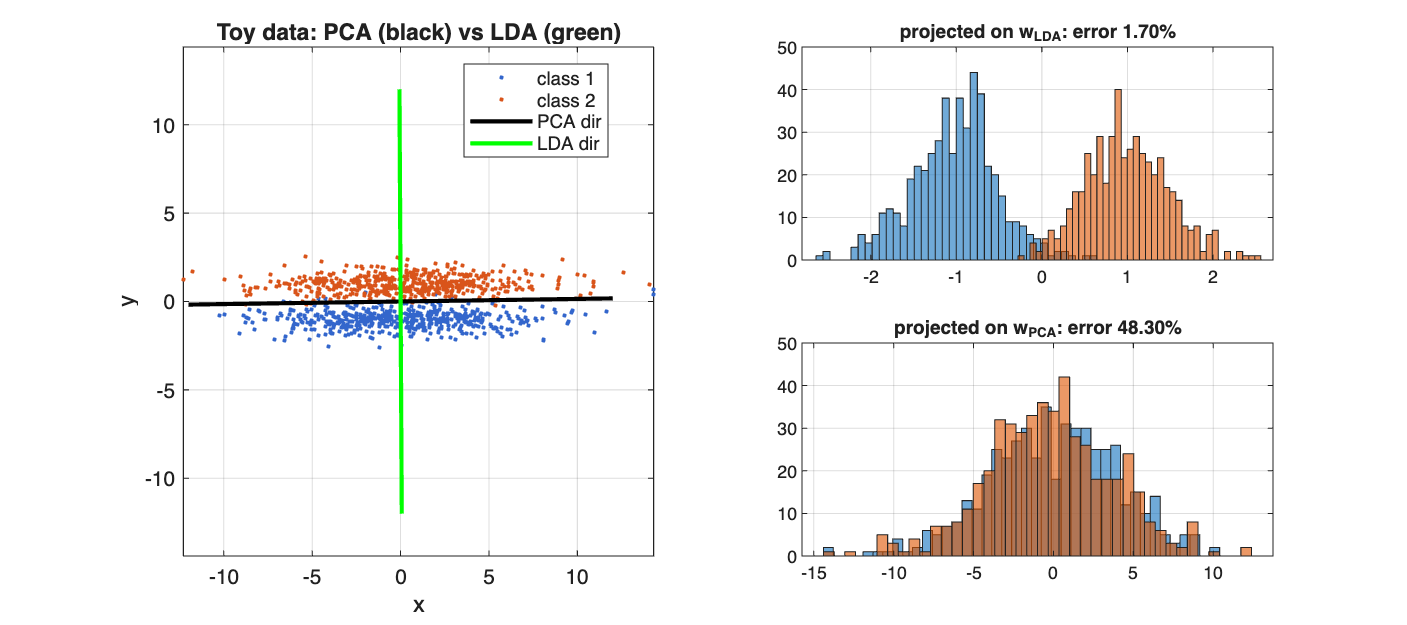
\includegraphics[width=0.95\textwidth]{figs/s1_toy.png}
\caption{S1: the same data, two directions. Black is the PCA direction (most
variance), green is the LDA direction (most separation). The right-hand panels show
the 1-D histograms after projection: on $w_{LDA}$ the classes separate cleanly, on
$w_{PCA}$ they sit on top of each other.}
\label{fig:toy}
\end{figure}

\section{Two classes: deriving the closed form}

\subsection{Setting up the criterion}

Let class $j$ have $n_j$ training points, mean $\mu_j$, and let $\bar{x}$ be the
overall mean. Define the \textbf{within-class scatter} and \textbf{between-class
scatter}
\[
  \Sw \;=\; \sum_{j=1}^{c}\;\sum_{x \in \text{class } j}(x-\mu_j)(x-\mu_j)^{\!\top},
  \qquad
  \Sb \;=\; \sum_{j=1}^{c} n_j\,(\mu_j-\bar{x})(\mu_j-\bar{x})^{\!\top}.
\]
Both are sums of outer products, hence symmetric and positive semi-definite.

Project onto a direction $w$. By the same one-line computation as in View~1, the
projected between-class spread is $w^{\!\top}\Sb w$ and the projected within-class
spread is $w^{\!\top}\Sw w$. Fisher's criterion is their ratio:
\[
  \boxed{\;J(w) \;=\; \frac{w^{\!\top}\Sb w}{w^{\!\top}\Sw w}\;}
\]
We want to make this as large as possible: means far apart (big numerator), classes
tight (small denominator).

\begin{gotcha}[The criterion is scale-invariant, so $\|w\|$ is meaningless]
Replace $w$ by $\alpha w$ for any $\alpha\ne 0$:
\[
  J(\alpha w) = \frac{\alpha^2 w^{\!\top}\Sb w}{\alpha^2 w^{\!\top}\Sw w} = J(w).
\]
The $\alpha^2$ cancels. So $J$ cares only about the \emph{direction} of $w$, and
the answer is a line through the origin, not a particular vector on it. This is why
we are free to normalise the Fisherfaces to unit length afterwards -- and why we
\emph{must} choose some convention, since nearest-neighbour distances do depend on
the scaling. A ratio like this is called a \emph{generalised Rayleigh quotient}.
\end{gotcha}

\subsection{Doing the maximisation}

Because of scale invariance we may fix the denominator and maximise the numerator:
\[
  \max_w\; w^{\!\top}\Sb w \quad\text{subject to}\quad w^{\!\top}\Sw w = 1 .
\]
Lagrangian:
\[
  \mathcal{L}(w,\lambda) = w^{\!\top}\Sb w - \lambda\,(w^{\!\top}\Sw w - 1).
\]
Both $\Sb$ and $\Sw$ are symmetric, so we may use
$\partial(w^{\!\top} Mw)/\partial w = 2Mw$ on each term:
\[
  \frac{\partial\mathcal{L}}{\partial w} = 2\Sb w - 2\lambda \Sw w = 0
  \qquad\Longrightarrow\qquad
  \boxed{\;\Sb w = \lambda\, \Sw w\;}
\]
This is a \textbf{generalised eigenvalue problem}. (If $\Sw=I$ it collapses to the
ordinary one.) Just as before, multiplying on the left by $w^{\!\top}$ identifies what
$\lambda$ is:
\[
  w^{\!\top}\Sb w = \lambda\,w^{\!\top}\Sw w
  \qquad\Longrightarrow\qquad
  \lambda = \frac{w^{\!\top}\Sb w}{w^{\!\top}\Sw w} = J(w).
\]
\textbf{The eigenvalue is the value of the criterion.} So we want the eigenvectors
with the largest $\lambda$, exactly as in PCA.

\subsection{The two-class closed form}\label{sec:twoclass}

With $c=2$ we can solve it by hand. First simplify $\Sb$. The overall mean is
$\bar{x}=\frac{n_1\mu_1+n_2\mu_2}{n_1+n_2}$, so
\[
  \mu_1-\bar{x} = \mu_1 - \frac{n_1\mu_1+n_2\mu_2}{n_1+n_2}
            = \frac{n_2(\mu_1-\mu_2)}{n_1+n_2},
  \qquad
  \mu_2-\bar{x} = \frac{n_1(\mu_2-\mu_1)}{n_1+n_2}.
\]
Writing $\delta := \mu_1-\mu_2$ and $n:=n_1+n_2$,
\[
  \Sb = n_1\frac{n_2^2}{n^2}\delta\delta^{\!\top} + n_2\frac{n_1^2}{n^2}\delta\delta^{\!\top}
      = \frac{n_1n_2(n_2+n_1)}{n^2}\,\delta\delta^{\!\top}
      = \frac{n_1n_2}{n}\,\delta\delta^{\!\top}.
\]
So for two classes $\Sb$ is a positive multiple of $\delta\delta^{\!\top}$, a
\textbf{rank-one} matrix. Substituting into $\Sb w=\lambda\Sw w$ and absorbing the
constant $\frac{n_1n_2}{n}$ into $\lambda$:
\[
  \delta\,(\delta^{\!\top} w) \;=\; \lambda' \,\Sw w .
\]
Now $\delta^{\!\top} w$ is a \emph{scalar}. Assuming $\Sw$ is invertible, multiply by
$\Sw^{-1}$:
\[
  \Sw^{-1}\delta\,(\delta^{\!\top} w) = \lambda' w
  \qquad\Longrightarrow\qquad
  w = \frac{\delta^{\!\top} w}{\lambda'}\;\Sw^{-1}\delta .
\]
The prefactor is just a scalar, and we established that scale does not matter, so
\[
  \boxed{\;w \;\propto\; \Sw^{-1}(\mu_1-\mu_2)\;}
\]
\paragraph{How to read this formula.} If $\Sw = I$ (classes are spherical), $w$
points straight from one mean to the other, which is the obvious answer.
$\Sw^{-1}$ corrects that naive guess for the shape of the classes: directions in
which the classes are already broadly smeared get \emph{down-weighted}. In our toy
data $\Sigma^{-1}=\operatorname{diag}(1/16,\,4)$ and $\mu_2-\mu_1=(0,2)^{\!\top}$, so
\[
  w \propto \operatorname{diag}(1/16,4)\,(0,2)^{\!\top} = (0,8)^{\!\top},
\]
the $y$ axis -- and the code prints $(-0.0054, 1.0000)$, agreeing.

\begin{observation}[We checked this is really the maximum]
Rather than trusting the algebra, section S1 tries \emph{every} direction
$(\cos t,\sin t)$ on a grid of $6283$ angles and takes the best:
\begin{lstlisting}
  brute-force best J over 6283 directions = 4.187363
  J(w_LDA) - J(brute) = 1.425e-05  (should be >= 0, up to grid step)
  |cos angle| between closed-form w and brute-force w = 0.99999997
\end{lstlisting}
The closed form beats the entire grid, and points in the same direction as the grid
winner to 7 decimal places. This is a direct numerical confirmation of the
derivation, and it needs no toolbox.
\end{observation}

\begin{observation}[Agreement with the theoretical Bayes error]
For two Gaussian classes with equal priors and a \emph{shared} covariance $\Sigma$,
the optimal (Bayes) error rate is $\Phi(-\Delta/2)$ where
$\Delta^2 = (\mu_2-\mu_1)^{\!\top}\Sigma^{-1}(\mu_2-\mu_1)$ is the Mahalanobis
distance between the means. Here
\[
  \Delta^2 = (0,2)\operatorname{diag}(1/16,4)(0,2)^{\!\top} = 16,\qquad \Delta = 4,
\]
so the Bayes error is $\Phi(-2)=2.28\%$. Our measured error along $w_{LDA}$ is
$1.70\%$, close to it (slightly below, because with $500$ samples per class the
empirical threshold happens to fit this particular sample a little better than the
population-optimal one). Along $w_{PCA}$ we measure $48.30\%$.

This is the strongest possible statement of LDA's optimality: \textbf{when the
classes really are Gaussian with equal covariance, LDA's 1-D projection loses
essentially nothing} compared to the best possible classifier in the full space.
\end{observation}

\begin{gotcha}
MATLAB's \texttt{normcdf} lives in the Statistics Toolbox, which is \emph{not}
installed on our machine. We compute $\Phi(-a)$ from the complementary error
function, which is in base MATLAB:
\[
  \Phi(-a) \;=\; \tfrac12\operatorname{erfc}\!\left(\frac{a}{\sqrt2}\right),
  \qquad\text{code: } \texttt{0.5 * erfc((delta/2)/sqrt(2))}.
\]
\end{gotcha}

\section{Many classes}

\subsection{The three scatter matrices and how they relate}

With $c$ classes we also define the \textbf{total scatter}
\[
  \St \;=\; \sum_{i=1}^{N}(x_i-\bar{x})(x_i-\bar{x})^{\!\top} .
\]
Note $\St = N\cdot C$: total scatter is total covariance without the $\frac1N$.

\begin{theorem}[Scatter decomposition]\label{thm:decomp}
$\St = \Sb + \Sw$.
\end{theorem}

\begin{proof}
Take any $x$ in class $j$ and insert $\mu_j$ twice:
\[
  x-\bar{x} = (x-\mu_j) + (\mu_j-\bar{x}).
\]
Write $u=x-\mu_j$ and $v=\mu_j-\bar{x}$. Then
\[
  (x-\bar{x})(x-\bar{x})^{\!\top} = (u+v)(u+v)^{\!\top} = uu^{\!\top} + uv^{\!\top} + vu^{\!\top} + vv^{\!\top}.
\]
Sum over the $n_j$ points of class $j$. The vector $v$ does not depend on which
point we are at, so it factors out of the cross terms:
\[
  \sum_{x\in j} uv^{\!\top} = \Bigl(\sum_{x\in j}(x-\mu_j)\Bigr)v^{\!\top} = 0\cdot v^{\!\top} = 0,
\]
because the deviations from a class's own mean sum to zero \emph{by the definition
of the mean}. The same kills $\sum vu^{\!\top}$. What is left is
\[
  \sum_{x\in j}(x-\bar{x})(x-\bar{x})^{\!\top} = \underbrace{\sum_{x\in j}(x-\mu_j)(x-\mu_j)^{\!\top}}_{\text{class $j$'s contribution to }\Sw} + \underbrace{n_j (\mu_j-\bar{x})(\mu_j-\bar{x})^{\!\top}}_{\text{class $j$'s contribution to }\Sb}.
\]
Summing over $j=1,\dots,c$ gives $\St=\Sw+\Sb$.
\end{proof}

\begin{observation}
Theorem~\ref{thm:decomp} is a free correctness test, and our code runs it every
time it builds the scatter matrices:
\begin{lstlisting}
info.resST = norm(St - (Sb + Sw), 'fro') / norm(St, 'fro');
\end{lstlisting}
Across all five dataset configurations the measured relative residual lies between
$2.7\times10^{-16}$ and $8.6\times10^{-16}$, i.e.\ machine precision. If a class
mean or a count $n_j$ were computed wrongly, this number would jump immediately.
\end{observation}

\subsection{The multi-class criterion}

With $c$ classes we want a whole projection \emph{matrix} $W\in\R^{d\times k}$, not
one direction. Projecting, the scatter matrices become $W^{\!\top}\Sb W$ and
$W^{\!\top}\Sw W$, which are $k\times k$ matrices -- so ``ratio'' needs a definition.
The standard choice is the ratio of determinants,
\[
  J(W) \;=\; \frac{\bigl|W^{\!\top}\Sb W\bigr|}{\bigl|W^{\!\top}\Sw W\bigr|} .
\]
The determinant is used because it is the product of the eigenvalues, i.e.\ the
\emph{volume} the scattered points occupy; so $J$ compares between-class volume to
within-class volume. The maximiser is the matrix whose columns are the $k$
generalised eigenvectors $\Sb w_l = \lambda_l \Sw w_l$ with the largest
$\lambda_i$ -- the same equation as the two-class case.

\begin{theorem}[The answer is a subspace, not a basis]\label{thm:invariance}
For any invertible $k\times k$ matrix $M$, $J(WM) = J(W)$.
\end{theorem}
\begin{proof}
$(WM)^{\!\top}\Sb(WM) = M^{\!\top}(W^{\!\top}\Sb W)M$, and determinants multiply, so
$|M^{\!\top}(W^{\!\top}\Sb W)M| = |M|^2\,|W^{\!\top}\Sb W|$. The same factor $|M|^2$ appears in
the denominator and cancels.
\end{proof}

\paragraph{Why this matters.} LDA pins down the \emph{subspace} spanned by the
Fisherfaces, but not which basis of it you get, and not the scaling of each basis
vector. Two correct implementations can return visibly different Fisherface
\emph{images} while defining the same projection. So ``my Fisherface pictures look
different from the paper's'' is not evidence of a bug.

\section{The rank theorems: why there are at most \texorpdfstring{$c-1$}{c-1} Fisherfaces}

\begin{theorem}\label{thm:rankSb}
$\rank(\Sb)\le c-1$.
\end{theorem}
\begin{proof}
$\Sb=\sum_{j=1}^c n_j(\mu_j-\bar{x})(\mu_j-\bar{x})^{\!\top}$ is a sum of $c$ rank-one matrices,
so immediately $\rank(\Sb)\le c$. Its column space is spanned by the $c$ vectors
$\mu_j-\bar{x}$. But those vectors satisfy one linear relation:
\[
  \sum_{j=1}^{c} n_j(\mu_j-\bar{x}) = \sum_j n_j\mu_j - \Bigl(\sum_j n_j\Bigr)\bar{x} = N\bar{x} - N\bar{x} = 0,
\]
using $\sum_j n_j\mu_j = \sum_i x_i = N\bar{x}$. A set of $c$ vectors with a non-trivial
linear dependence spans a space of dimension at most $c-1$. Hence
$\rank(\Sb)\le c-1$.
\end{proof}

\begin{corollary}[The hard ceiling]
Since $\Sb w=\lambda\Sw w$ forces $\lambda=0$ whenever $w$ lies in the null space of
$\Sb$, at most $c-1$ generalised eigenvalues are non-zero. \textbf{There are at
most $c-1$ useful Fisherfaces, however many pixels or training images we have.}
\end{corollary}

For ORL-32 that is $31$; for ORL-40, $39$; for Yale, $37$.

\begin{observation}
Section S12(d) measures it:
\begin{lstlisting}
  (d) ORL-32: c = 32, so theory says rank(S_B) <= 31
      measured rank(S_B) = 31, number of fisherfaces = 31
\end{lstlisting}
The bound is tight here.
\end{observation}

\begin{theorem}\label{thm:rankSw}
$\rank(\Sw)\le N-c$.
\end{theorem}
\begin{proof}
Let $A_W$ be the $d\times N$ matrix whose columns are the within-class-centred
images $x_j-\mu_{\text{class}(i)}$. Then $\Sw=A_WA_W^{\!\top}$, so
$\rank(\Sw)=\rank(A_W)$.

Group the columns by class. Within class $j$, the $n_j$ columns sum to zero (again
by the definition of $\mu_j$), so those $n_j$ columns span a space of dimension at
most $n_j-1$. Summing over classes,
\[
  \rank(A_W)\;\le\;\sum_{j=1}^{c}(n_j-1) \;=\; \Bigl(\sum_j n_j\Bigr) - c \;=\; N-c. \qedhere
\]
\end{proof}

\paragraph{The degrees-of-freedom reading -- remember this one.}
The proof says each class donates only $n_j-1$ directions to $\Sw$. So:
\begin{itemize}[nosep]
\item ORL with $6$ images per person: each class contributes $\mathbf{5}$ directions.
\item Yale with $40$ images per person: each class contributes $\mathbf{39}$.
\end{itemize}
$\Sw$ is our estimate of ``how a person's images vary''. On ORL that estimate is
built from five directions per person, which is almost nothing. This single fact
predicts most of what we observe in Part~V, including why Fisherfaces \emph{lose}
on ORL.

\begin{observation}[Measured --- and how a dataset defect showed up in the rank]
Section S5 computes $\rank(\Sw)$ for Yale without ever forming the $d\times d$
matrix, by using $\rank(A_WA_W^{\!\top})=\rank(A_W)=\rank(A_W^{\!\top} A_W)$ and
working with the small $N\times N$ Gram matrix instead:
\begin{lstlisting}
  Yale: d = 32256, N = 1520, c = 38
  S_W in pixel space would be 32256 x 32256 = 8.32 GB
  theory: rank(S_W) <= N - c = 1482
  measured rank(S_W)         = 1482
\end{lstlisting}

On our \emph{first} run the measured rank came out as $\mathbf{1481}$ -- one \emph{less}
than the bound. Rather than wave it away, we tracked it down. A rank deficiency
beyond the predicted one means some class has an \emph{exact} linear dependency
among its images, and the simplest way that happens is a repeated image. Adding a
duplicate search to the script found exactly one pair, in subject 12. The culprit
was a stray file in our copy of the database,
\begin{center}
\texttt{CroppedYale/yaleB12/yaleB12\_P00A+020E+10 - Copy.pgm}
\end{center}
byte-identical to \texttt{yaleB12\_P00A+020E+10.pgm} -- somebody had accidentally
duplicated a file inside the dataset. Two identical columns stay identical after
within-class centring, so they are an exact linear dependency and cost exactly one
unit of rank: $1482-1 = 1481$, which is what we measured.

We removed the stray file and re-ran everything. The rank now meets the bound
exactly, and the duplicate search reports none. All numbers in this document come
from the cleaned dataset.

Two lessons worth carrying: $N-c$ is an \emph{upper} bound that real data can fall
short of through repeated or linearly dependent images; and a rank that disagrees
with theory by a small amount is usually telling you something true about the data
rather than about the algorithm.
\end{observation}

\begin{gotcha}
Removing that file also changed the \emph{split}, which is a subtler effect than it
first appears. \texttt{dir} sorts alphabetically, and the string
\texttt{'yaleB12\_P00A+020E+10 - Copy.pgm'} sorts \emph{before}
\texttt{'yaleB12\_P00A+020E+10.pgm'} (a space, ASCII 32, is smaller than the dot,
ASCII 46). So the duplicate used to sit inside subject 12's first 40 files, i.e.\
inside the training set, and deleting it pulls one previously-unseen image forward
from test into train for that one subject. Changing a dataset is never only a
change to the data: here it silently moved one image across the train/test
boundary.
\end{gotcha}

\part{Fisherfaces}

\section{The small-sample-size problem}

Fisher's LDA needs $\Sw^{-1}$. For face images that is impossible, for two separate
reasons, and it is important to keep them apart because they have different fixes.

\begin{enumerate}[label=(\arabic*)]
\item \textbf{Size.} $\Sw$ is $d\times d$. For Yale, $32256^2$ doubles is
  $\mathbf{8.3}$~GB. We cannot store it, never mind invert it (cost $O(d^3)
  \approx 3\times10^{13}$ operations).
\item \textbf{Rank.} By Theorem~\ref{thm:rankSw}, $\rank(\Sw)\le N-c = 1482$,
  while $d=32256$. So $\Sw$ is singular by a margin of more than $30{,}000$
  dimensions. $\Sw^{-1}$ \emph{does not exist}. This is not a numerical difficulty
  that a better algorithm could dodge; it is a statement about the data.
\end{enumerate}

This is the \textbf{small-sample-size problem}: we have far more measurements per
sample ($d$) than samples ($N$). Note that (2) is not fixed by more computer
memory. It is fixed only by reducing the dimension or by changing the estimator.

\section{The two-stage algorithm}

The paper's solution is to project into a space where $\Sw$ \emph{is} invertible,
and do LDA there.

\begin{enumerate}[label=\textbf{Stage \arabic*.},leftmargin=*]
\item \textbf{PCA to $m$ dimensions.} Compute the eigenfaces of the total scatter
  and keep the top $m$, giving $W_{\text{pca}}\in\R^{d\times m}$. The paper takes
  $m=N-c$.
\item \textbf{LDA inside that space.} Form $\Sb$ and $\Sw$ from the projected
  training data (now $m\times m$ matrices, small enough to handle), solve
  $\Sb w=\lambda\Sw w$ and keep the top $c-1$ eigenvectors as
  $W_{\text{fld}}\in\R^{m\times(c-1)}$.
\end{enumerate}

The two projections compose into a single one:
\[
  W_{\text{opt}}^{\!\top} \;=\; W_{\text{fld}}^{\!\top}\,W_{\text{pca}}^{\!\top},
  \qquad\text{i.e.}\qquad
  W_{\text{opt}} \;=\; W_{\text{pca}}\,W_{\text{fld}} \;\in\; \R^{d\times(c-1)}.
\]
To classify an image $x$ we compute $W_{\text{opt}}^{\!\top}(x-\bar{x})\in\R^{c-1}$ and find
its nearest training neighbour. The columns of $W_{\text{opt}}$, viewed as images,
are the \textbf{Fisherfaces}.

\subsection{Why \texorpdfstring{$m=N-c$}{m = N-c}?}

A rank argument, from both sides:
\begin{itemize}[nosep]
\item If $m > N-c$: the projected $\Sw$ is $m\times m$ but still has rank at most
  $N-c < m$ (projection cannot increase rank), so it is \emph{still singular}. We
  have gained nothing.
\item If $m = N-c$: the projected $\Sw$ is $(N-c)\times(N-c)$ with rank at most
  $N-c$, so generically it is exactly full rank and invertible.
\item If $m < N-c$: $\Sw$ is invertible too, but we have thrown away some
  directions of the data before LDA ever saw them.
\end{itemize}
So $m=N-c$ is the \emph{largest} choice that makes $\Sw$ invertible. The paper
picks it to discard as little as possible.

\subsection{The zero-slack problem with that choice}\label{sec:zeroslack}

Here is the catch, and it is the most important ``why this and not that'' in the
whole project.

At $m=N-c$, the rank of $\Sw$ equals its dimension \emph{exactly}. There is no
slack. The last few eigenvalues of $\Sw$ are built from almost no data -- they are
the directions in which the training set happened to vary least -- so they are
essentially estimation noise. And $\Sw^{-1}$ \textbf{divides} by them, so it
amplifies precisely the directions we know least about.

``Invertible'' and ``well conditioned'' are not the same thing. The condition
number
\[
  \kappa(\Sw) = \frac{\lambda_{\max}(\Sw)}{\lambda_{\min}(\Sw)}
\]
measures how badly inversion amplifies error. Our sweep in section S9 measures it
directly as $m$ grows, and the growth is dramatic -- see Section~\ref{sec:msweep}.
On Yale it reaches $\kappa \approx 2\times10^{11}$ at $m=N-c$, up from
$2.6\times10^{6}$ at $m=1200$; in double precision (about $16$ significant digits)
that leaves the smallest eigenvalues of $\Sw$ with only about five correct digits,
and $\Sw^{-1}$ divides by exactly those.

\textbf{Conclusion:} $m=N-c$ is the right answer to ``what is the largest $m$ that
makes $\Sw$ invertible'' but the wrong answer to ``what value of $m$ gives the best
recogniser''. We show this empirically in Section~\ref{sec:msweep}.

\section{The generalised eigenvalue problem}
\label{sec:gevp}

Everything in Part~II ended at the same equation, $\Sb w = \lambda \Sw w$. It is
worth stopping to study that object in its own right, because all the structural
facts about Fisherfaces --- how many there are, why the eigenvalues are real, why
the Fisherfaces are $\Sw$-orthogonal and not Euclidean-orthogonal, and what
exactly goes wrong when $\Sw$ is singular --- are properties of this problem, not
of faces.

\subsection{Definition, and the three cases}

\begin{definition}
Given two $m\times m$ matrices $A$ and $B$, the pair $(A,B)$ is called a
\emph{matrix pencil}. A scalar $\lambda$ and a vector $w \neq 0$ with
\[
  A w \;=\; \lambda\, B w
\]
are a \emph{generalised eigenvalue} and \emph{generalised eigenvector} of the
pencil. Setting $B=I$ recovers the ordinary eigenproblem.
\end{definition}

For us $A=\Sb$ and $B=\Sw$. Three cases behave very differently, and knowing
which one you are in is the whole game:

\begin{enumerate}[leftmargin=*,label=(\alph*)]
\item \textbf{$B$ nonsingular.} The problem is equivalent to the ordinary
  eigenproblem for $B^{-1}A$ and has exactly $m$ finite eigenvalues. This is the
  case the two-stage recipe manufactures by projecting to $m=N-c$ dimensions.
\item \textbf{$B$ singular, but $A$ and $B$ share no null vector.} Take $w$ with
  $Bw = 0$ and $Aw \neq 0$. Then $Aw = \lambda Bw = 0$ has no finite solution, and
  the convention is to say the pencil has an \emph{infinite} eigenvalue. The
  pencil still makes sense, but has fewer than $m$ finite eigenvalues.
\item \textbf{$A$ and $B$ share a null vector.} If $Aw = Bw = 0$ for some
  $w\neq0$, then $Aw = \lambda Bw$ holds for \emph{every} $\lambda$. The pencil is
  called \emph{singular} and its eigenvalues are simply not defined. This is the
  genuinely bad case.
\end{enumerate}

\begin{gotcha}[Case (b) is not a disaster --- it is null-space LDA]
An infinite eigenvalue means a direction $w$ with $w^{\!\top}\Sw w = 0$ but
$w^{\!\top}\Sb w > 0$: the classes have \emph{zero} spread along it and their means
still differ. The Fisher criterion $J(w)$ is then infinite --- a perfectly
discriminative direction, at least on the training set. Chasing exactly these
directions is what null-space LDA (Section~\ref{sec:alternatives}) does. The
reason we do not is that with $d\gg N$ there are tens of thousands of such
directions and almost all of them are accidents of having too few samples.
\end{gotcha}

\begin{gotcha}[Case (c) is what $m>N-c$ actually produces]
Beyond $m = N-c$ the matrices $\Sw$ and $\Sb$ do share null vectors, so the pencil
becomes singular in the technical sense above and ``the eigenvalues'' stop being a
well-posed question. That is the real reason the recipe caps $m$ at $N-c$ --- not
merely that $\Sw^{-1}$ fails to exist, but that the problem itself stops having a
unique answer. It is also why \texttt{chol} refusing (Section~\ref{sec:alternatives})
is the right behaviour rather than an inconvenience.
\end{gotcha}

\subsection{The good case: a symmetric-definite pencil}

Our pencil, after the PCA stage, has more structure than a general one:
$\Sb$ is symmetric positive semi-definite, and $\Sw$ is symmetric
\emph{positive definite}. Such a pair is called a \textbf{symmetric-definite
pencil}, and it is as well behaved as the ordinary symmetric eigenproblem.

\begin{theorem}[Simultaneous diagonalisation]
\label{thm:simdiag}
Let $A$ be symmetric and $B$ symmetric positive definite, both $m\times m$. Then
there is a nonsingular $W\in\R^{m\times m}$ with
\[
  W^{\!\top} B\, W \;=\; I,
  \qquad
  W^{\!\top} A\, W \;=\; \Lambda = \operatorname{diag}(\lambda_1,\dots,\lambda_m),
\]
all $\lambda_l$ real, and the columns of $W$ satisfy $A w_l = \lambda_l B w_l$.
\end{theorem}

\begin{proof}
Because $B$ is symmetric positive definite it has a Cholesky factorisation
$B = R^{\!\top}R$ with $R$ upper triangular and invertible. Define
\[
  M \;:=\; R^{-\top} A\, R^{-1}.
\]
$M$ is symmetric, since
$M^{\!\top} = R^{-\top}A^{\!\top}R^{-1} = R^{-\top}AR^{-1} = M$ using $A^{\!\top}=A$.
By the spectral theorem a real symmetric matrix can be written $M = Z\Lambda Z^{\!\top}$
with $Z$ orthogonal ($Z^{\!\top}Z=I$) and $\Lambda$ real diagonal. Now set
\[
  W \;:=\; R^{-1}Z ,
\]
which is nonsingular as a product of nonsingular matrices. Check the two claims
directly:
\[
  W^{\!\top} B W = Z^{\!\top}R^{-\top}\,(R^{\!\top}R)\,R^{-1}Z = Z^{\!\top}Z = I,
\]
\[
  W^{\!\top} A W = Z^{\!\top}R^{-\top} A R^{-1} Z = Z^{\!\top} M Z = \Lambda .
\]
For the last claim, start from $Mz_l = \lambda_l z_l$, i.e.\
$R^{-\top}AR^{-1}z_l = \lambda_l z_l$, and multiply on the left by $R^{\!\top}$:
\[
  A R^{-1} z_l \;=\; \lambda_l R^{\!\top} z_l .
\]
Since $w_l = R^{-1}z_l$, equivalently $z_l = Rw_l$, this reads
$A w_l = \lambda_l R^{\!\top}R\, w_l = \lambda_l B w_l$.
\end{proof}

Three consequences fall straight out, and they are exactly the facts used
elsewhere in this guide.

\begin{corollary}[Real eigenvalues]
The $\lambda_l$ are real, because they are the eigenvalues of the real symmetric
matrix $M$. No symmetry assumption about $B^{-1}A$ is needed --- indeed $B^{-1}A$
is generally \emph{not} symmetric, which is why the naive route
(Section~\ref{sec:routes}) has no such guarantee.
\end{corollary}

\begin{corollary}[$B$-orthogonality]
$W^{\!\top}BW = I$ says precisely $w_l^{\!\top}B\,w_{l'} = \delta_{ll'}$. With
$B=\Sw$ this is the $\Sw$-orthogonality of the Fisherfaces. They are orthonormal
in the inner product $\langle u,v\rangle_{\Sw} = u^{\!\top}\Sw v$, and there is no
reason for them to be orthonormal in the ordinary one --- that would need
$\Sw = I$.
\end{corollary}

\begin{corollary}[How many non-zero eigenvalues]
$M = R^{-\top}\Sb R^{-1}$ is a \emph{congruence} transformation of $\Sb$ by an
invertible matrix, and congruence preserves rank. So
$\rank(M) = \rank(\Sb) \le c-1$ by Theorem~\ref{thm:rankSb}, and the pencil has at
most $c-1$ non-zero eigenvalues however large $m$ is. The remaining $m-(c-1)$ are
zero, and their eigenvectors are an arbitrary basis of a null space --- which is
why we keep only the first $c-1$ columns.
\end{corollary}

\begin{observation}[The rank bound is visible as a cliff in the spectrum]
Section S12(e) computes all $m=160$ generalised eigenvalues of $(\Sb,\Sw)$ on
ORL-32, where $c-1 = 31$:
\begin{center}
\begin{tabular}{lr}
\toprule
$\lambda_1,\lambda_2,\lambda_3$ & $1.49\times10^{7}$, \; $7.15\times10^{4}$, \; $1.81\times10^{4}$ \\
$\lambda_{30}, \lambda_{31}$ \;(last two allowed to be non-zero) & $13.72$, \; $7.47$ \\
$\lambda_{32}$ \;(first that \emph{must} vanish) & $2.10\times10^{-12}$ \\
largest $|\lambda_l|$ for $l \ge 32$ & $2.87\times10^{-12}$ \\
\midrule
$\lambda_1 \,/\, \max_{l\ge32}|\lambda_l|$ & $5.21\times10^{18}$ \\
\bottomrule
\end{tabular}
\end{center}
Between $\lambda_{31}=7.47$ and $\lambda_{32}=2.1\times10^{-12}$ the spectrum
falls off a cliff of roughly \textbf{twelve orders of magnitude}, and every
eigenvalue past index $31$ is at the level of round-off. The corollary is not an
abstract bound that happens to hold --- it shows up as a visible discontinuity in
the numbers, exactly at $l = c-1$.

Two things follow. The eigenvalues past $c-1$ being $10^{-12}$ rather than exactly
$0$ is ordinary floating-point noise, not a rank violation. And their
eigenvectors are an arbitrary basis of a null space, so keeping them would add
pure noise as ``discriminant directions'' --- which is why the code truncates at
$c-1$ rather than trusting the solver's ordering.
\end{observation}

\subsection{Why the eigenvalue \emph{is} the criterion}

We asserted this in Part~II; here is the clean statement and proof.

\begin{theorem}[Generalised Rayleigh quotient]
\label{thm:rayleigh}
For a symmetric-definite pencil $(A,B)$,
\[
  \max_{w\neq0}\; \frac{w^{\!\top}Aw}{w^{\!\top}Bw} \;=\; \lambda_{\max},
\]
attained at the corresponding generalised eigenvector. More generally the $l$th
largest value, maximised over directions $B$-orthogonal to the first $l-1$
eigenvectors, is $\lambda_l$.
\end{theorem}

\begin{proof}
Substitute $w = R^{-1}z$; since $R$ is invertible this is a bijection between
non-zero $w$ and non-zero $z$, so it cannot change the maximum. The numerator and
denominator become
\[
  w^{\!\top}Aw = z^{\!\top}R^{-\top}AR^{-1}z = z^{\!\top}Mz,
  \qquad
  w^{\!\top}Bw = z^{\!\top}R^{-\top}\,(R^{\!\top}R)\,R^{-1}z = z^{\!\top}z .
\]
So the generalised Rayleigh quotient of $(A,B)$ at $w$ equals the \emph{ordinary}
Rayleigh quotient of $M$ at $z$:
\[
  \frac{w^{\!\top}Aw}{w^{\!\top}Bw} \;=\; \frac{z^{\!\top}Mz}{z^{\!\top}z}.
\]
The ordinary Rayleigh quotient of a symmetric matrix is maximised by its top
eigenvector and equals its top eigenvalue --- which is the $B=I$ case we already
proved in Section~\ref{sec:view1}. Mapping back through $w = R^{-1}z$ gives the
result, and the eigenvalues of $M$ are the generalised eigenvalues of $(A,B)$ by
Theorem~\ref{thm:simdiag}.
\end{proof}

With $A=\Sb$, $B=\Sw$ this says $\lambda_l = J(w_l)$: \textbf{the $l$th
generalised eigenvalue is literally the Fisher criterion value of the $l$th
Fisherface.} Sorting eigenvalues descending is sorting discriminant directions by
how well they separate the classes, and nothing more mysterious.

\subsection{A note on how software reports these}

Numerical libraries avoid dividing by zero by returning eigenvalues as
\emph{pairs} $(\alpha_l, \beta_l)$ with
\[
  \beta_l\, A w_l \;=\; \alpha_l\, B w_l , \qquad \lambda_l = \alpha_l/\beta_l ,
\]
so that $\beta_l = 0$ encodes the infinite eigenvalue of case (b) without
overflowing. MATLAB's \texttt{eig(A,B)} hides this and hands back $\lambda$
directly, returning \texttt{Inf} where $\beta_l=0$; the QZ algorithm it uses
underneath works with the pair. This is why route 5 of Section~\ref{sec:routes}
can run even when $B$ is singular, while \texttt{chol} refuses --- QZ does not
need $B^{-1}$ to exist.

\section{What the paper specifies, and what it leaves to you}
\label{sec:paperscope}

Before comparing solvers it is worth being clear about how much of this the
original paper actually prescribes, because ``why did you do it \emph{this}
way?'' has a different answer depending on whether the paper made the choice or
we did. We checked the published text rather than relying on memory.

\paragraph{On the generalised eigenproblem: nothing at all.}
The paper's complete treatment is two sentences. It defines the solution as
\begin{quote}
``where $w_i \mid i=1,2,\ldots,m$ is the set of generalized eigenvectors of
$\Sb$ and $\Sw$ corresponding to the $m$ largest generalized eigenvalues
$\lambda_i$, i.e., $\Sb w_i = \lambda_i \Sw w_i$''
\end{quote}
and then bounds how many there are:
\begin{quote}
``Note that there are at most $c-1$ nonzero generalized eigenvalues, and so an
upper bound on $m$ is $c-1$, where $c$ is the number of classes. See [4].''
\end{quote}
Reference [4] is Duda \& Hart, \emph{Pattern Classification and Scene
Analysis} (1973) --- a pattern-recognition textbook, cited for the \emph{rank
bound}, not for numerics. Searching the full text finds \textbf{no} mention of
Cholesky factorisation, whitening, simultaneous diagonalisation, the QZ
algorithm, pseudo-inverses, or any numerical library, and the bibliography
contains no numerical-linear-algebra reference at all. The authors state
\emph{what} to compute and leave \emph{how} to the reader's library.

Everything in Section~\ref{sec:solve} is therefore ours, not the paper's. That
is the honest answer to ``why Cholesky?'': the paper does not say, so we chose,
and Section~\ref{sec:routes} measures the consequences of the choice.

\paragraph{On the singularity of $\Sw$: explicit, and it matches our account.}
Here the paper is precise, and note that its criterion is \emph{conditional}:
``If $\Sw$ is nonsingular, the optimal projection $W_{opt}$ is chosen as\ldots''
It then explains why that condition fails for faces:
\begin{quote}
``one is confronted with the difficulty that the within-class scatter matrix
$\Sw \in \mathbb{R}^{n\times n}$ is always singular. This stems from the fact
that the rank of $\Sw$ is at most $N-c$, and, in general, the number of images
in the learning set $N$ is much smaller than the number of pixels in each image
$n$.''
\end{quote}
and gives exactly one remedy:
\begin{quote}
``projecting the image set to a lower dimensional space so that the resulting
within-class scatter matrix $\Sw$ is nonsingular. This is achieved by using PCA
to reduce the dimension of the feature space to $N-c$, and then applying the
standard FLD \ldots to reduce the dimension to $c-1$.''
\end{quote}
This is the resolution of the apparent paradox in Section~\ref{sec:routes}: how
can route~1 invert $\Sw$ when $\Sw$ is singular? Because singularity is a
statement about the $n\times n$ pixel-space matrix, and by the time any solver
runs we are in the reduced $m$-dimensional space where $\Sw$ has full rank $m$.
The $m$-sweep in Section~\ref{sec:msweep} shows $\operatorname{rank}(\Sw)=m$ on
every row.

\paragraph{On regularisation: the paper has none.}
No ridge, no $\varepsilon I$, no pseudo-inverse appears anywhere in it.
Dimension reduction is its only fix. The regularised path in our code is a
fallback we added, and Section~\ref{sec:alternatives} is a comparison the paper
does not make.

\paragraph{One thing the paper proposes but does not do.}
Its equation (6) is null-space LDA, and it is explicitly unfinished work:
\begin{quote}
``a second method \emph{which we are currently investigating} chooses $W$ to
maximize the between-class scatter of the projected samples after having first
reduced the within-class scatter. Taken to an extreme, we can maximize the
between-class scatter of the projected samples subject to the constraint that
the within-class scatter is zero''
\end{quote}
over ``the set of $n\times m$ matrices with orthonormal columns contained in the
kernel of $\Sw$''. That is precisely case~(b) of
Section~\ref{sec:gevp} --- a singular $B$ with no shared null vector, giving
$J(w)=\infty$. Section~\ref{sec:alternatives} explains it and says why we did
not implement it either: on Yale that kernel has $d-(N-c)=30774$ dimensions, so
``zero within-class scatter'' there is mostly an artefact of having too few
samples. So this is one alternative that neither the paper nor we measured, and
it should be described that way rather than claimed as a result.

\begin{gotcha}[The paper says ``orthonormal columns'', and strictly it should not]
The paper states that ``the optimization for $W_{fld}$ is performed over
$(N-c)\times m$ matrices \textbf{with orthonormal columns}''. But the
generalised eigenvectors its own equation~(4) defines are
$\Sw$-orthogonal: they satisfy $W^{\!\top}\Sw W = I$, not $W^{\!\top}W = I$, and
the two coincide only when $\Sw = I$. The slip is harmless, because $J(W)$ is
invariant under any nonsingular change of basis
(Theorem~\ref{thm:invariance}), so rescaling columns changes neither the
subspace nor the recognition rate. But it is still a slip: if asked ``are
Fisherfaces orthogonal?'', the answer is \emph{not} ``yes, the paper says
orthonormal columns.'' They are orthogonal in the $\Sw$ inner product and
generally not in the Euclidean one --- which our code confirms, measuring
$\|W^{\!\top}\Sw W - I\|/\sqrt{c-1} = 4.61\times10^{-12}$.
\end{gotcha}

\section{Solving \texorpdfstring{$\Sb w=\lambda\Sw w$}{Sb w = lambda Sw w} properly}
\label{sec:solve}

\subsection{The naive route, and what is actually wrong with it}
\label{sec:naive}

The obvious move is to multiply by $\Sw^{-1}$ and solve the ordinary eigenproblem
\[
  \Sw^{-1}\Sb\,w = \lambda w .
\]
This is mathematically fine. The objection is structural: the product
$\Sw^{-1}\Sb$ is generally \textbf{not symmetric}, even though $\Sw$ and $\Sb$
both are, because
\[
  (\Sw^{-1}\Sb)^{\!\top} \;=\; \Sb^{\!\top}\Sw^{-\top} \;=\; \Sb\,\Sw^{-1},
\]
and $\Sb\Sw^{-1} \neq \Sw^{-1}\Sb$ unless the two matrices happen to commute.
So MATLAB has to call a general non-symmetric eigensolver, and three guarantees
are lost: eigenvalues may come back complex from pure round-off even though the
true ones are real and non-negative; the eigenvectors are not orthogonal in
\emph{any} inner product; and we have formed $\Sw^{-1}$ explicitly, with
$\kappa(\Sw)\approx 10^{11}$.

\paragraph{But how bad is it \emph{here}? Measured: not bad at all.}
It would be dishonest to leave the above as the answer, because we ran it.
Route~1 of Section~\ref{sec:routes} is exactly this naive computation, and on
the harder of our two problems --- Yale with $m=1482$ and
$\kappa(\Sw)=4.19\times10^{11}$ --- it gives:

\begin{center}
\begin{tabular}{lccc}
\toprule
route & rate & $\max|\operatorname{Im}\lambda|$ & angle vs.\ Cholesky \\
\midrule
1. $\mathtt{inv(Sw)*Sb}$, then \texttt{eig} & 95.5\% & $8.43\times10^{-9}$ & $0.00^\circ$ \\
3. Cholesky whitening (ours)                & 95.5\% & $0$                 & --- \\
\bottomrule
\end{tabular}
\end{center}

The imaginary parts are at round-off, the recovered subspace agrees with the
Cholesky one to $0.00^\circ$, and the recognition rate is \emph{identical}. The
same holds on ORL. \textbf{The naive route is not wrong for our data.} Anyone claiming
otherwise is reciting a rule instead of reporting a measurement.

\paragraph{Why it survives, mechanically.} This is the part worth understanding,
because it tells us when the naive route \emph{would} fail. Eigenvector accuracy
in a non-symmetric problem degrades as the \emph{gap} between an eigenvalue and
its neighbours shrinks relative to the size of the matrix. Our wanted
eigenvalues are not crowded --- from Section~\ref{sec:gevp} the top three on
ORL are $1.49\times10^{7}$, $7.15\times10^{4}$, $1.81\times10^{4}$, each
separated from the next by orders of magnitude, and everything past
$l=c-1$ sits at $10^{-12}$. We only ever keep the top $c-1$, i.e.\ the
best-separated end of the spectrum. The ill-conditioning of $\Sw$ does inject
error, but it lands in the directions we throw away.

\paragraph{So why do we still not use it?} Three reasons, in order of honesty.

\begin{enumerate}[nosep]
\item \textbf{It has no guarantee, it just happened to work.} The bound on the
  non-symmetric solver's error involves $\kappa(\Sw)$; we got a good answer
  because the spectrum is favourably spread, not because the method promised
  one. Change $m$, the dataset, or the number of images per class and the gaps
  close. The symmetric route's accuracy does not depend on that luck.
\item \textbf{The output needs cleaning up, and the theory no longer applies to
  what you computed.} You must call \texttt{real()} on the eigenvalues, re-sort,
  and accept eigenvectors that satisfy no orthogonality relation. In particular
  the simultaneous-diagonalisation theorem (Theorem~\ref{thm:simdiag}) says the
  true $W$ satisfies $W^{\!\top}\Sw W = I$; the vectors route~1 returns satisfy
  that only up to whatever the solver did. We lose the ability to \emph{check}
  our own answer.
\item \textbf{It is the slowest route.} Measured on Yale: $2.68$\,s versus
  $1.01$\,s for Cholesky. Quote the \emph{ratio}, not the seconds --- across
  three runs of the script the absolute times moved by nearly $3\times$
  ($0.93$, $2.16$, $2.68$\,s for route~1) because the machine was not otherwise
  idle, while the ratio stayed put at $2.58$, $2.81$, $2.65$. A single
  wall-clock number is not a reproducible measurement; a ratio measured inside
  one run largely is. Forming $\Sw^{-1}$
  ($\sim m^3$ work) and then running a non-symmetric QR iteration is strictly
  more arithmetic than one Cholesky factorisation plus a symmetric
  tridiagonal eigensolve.
\end{enumerate}

\paragraph{The viva answer, in one sentence.} ``The naive route gave bit-for-bit
the same recognition rate and the same subspace to $0.00^\circ$ on both
datasets, so it is not wrong here; we use Cholesky whitening because it is
$2.7\times$ faster, needs no post-processing, and its accuracy does not depend
on the eigenvalue gaps happening to be large.''

\subsection{Cholesky whitening: the route we use}

Because $\Sw$ is symmetric positive definite, it has a \textbf{Cholesky
factorisation} $\Sw=R^{\!\top} R$ with $R$ upper triangular and invertible. Now
substitute $w=R^{-1}z$ into $\Sb w=\lambda\Sw w$:
\[
  \Sb R^{-1}z \;=\; \lambda\, \Sw R^{-1} z \;=\; \lambda\, R^{\!\top} R R^{-1} z \;=\; \lambda\, R^{\!\top} z .
\]
Multiply on the left by $R^{-\top} := (R^{\!\top})^{-1}$:
\[
  \boxed{\;\underbrace{R^{-\top}\Sb R^{-1}}_{=:\,M}\,z \;=\; \lambda\, z\;}
\]
and $M$ \textbf{is symmetric}, because
$M^{\!\top} = (R^{-\top}\Sb R^{-1})^{\!\top} = R^{-\top}\Sb^{\!\top} R^{-1} = R^{-\top}\Sb R^{-1} = M$,
using $\Sb^{\!\top}=\Sb$. So we now have an ordinary \emph{symmetric} eigenproblem,
for which:
\begin{itemize}[nosep]
\item eigenvalues are guaranteed real;
\item eigenvectors are guaranteed orthogonal;
\item the algorithm is backward stable.
\end{itemize}
Having found $z$, recover $w = R^{-1}z$, i.e.\ solve $Rw=z$ (cheap: $R$ is
triangular). Note the eigen\emph{values} $\lambda$ are unchanged by the
substitution, so they are still exactly the Fisher criterion values.

\paragraph{Upper or lower triangular? Either --- they are the same factorisation.}
Many textbooks write Cholesky as $\Sw = LL^{\!\top}$ with $L$ \emph{lower}
triangular, and that is an equally valid starting point. The two conventions are
related by one transpose: if $\Sw = R^{\!\top}R$ with $R$ upper triangular, then
$L := R^{\!\top}$ is lower triangular and
\[
  LL^{\!\top} \;=\; R^{\!\top}\!\left(R^{\!\top}\right)^{\!\top} \;=\; R^{\!\top}R \;=\; \Sw ,
\]
so $L$ is \emph{the same numbers}, just stored as the transpose. Running the
derivation in the lower-triangular convention, substitute $w = L^{-\top}z$ into
$\Sb w = \lambda \Sw w$:
\[
  \Sb L^{-\top} z \;=\; \lambda\, LL^{\!\top}L^{-\top} z \;=\; \lambda\, L z ,
\]
then multiply on the left by $L^{-1}$:
\[
  \underbrace{L^{-1}\Sb L^{-\top}}_{=:\,M_L} z \;=\; \lambda z ,
\]
and $M_L$ is symmetric by the same one-line argument:
$M_L^{\!\top} = (L^{-1}\Sb L^{-\top})^{\!\top} = L^{-1}\Sb^{\!\top}L^{-\top} = M_L$.
Substituting $L = R^{\!\top}$ gives
$M_L = R^{-\top}\Sb R^{-1} = M$ --- \textbf{literally the same matrix}, so the
same eigenvalues and the same $\lambda_l = J(w_l)$. The only thing that changes
is the recovery step: upper gives $w = R^{-1}z$ (solve $Rw=z$), lower gives
$w = L^{-\top}z$ (solve $L^{\!\top}w = z$), and those are the same linear system
written twice.

\paragraph{Measured, not asserted.} Section S12(f) of the script runs both
conventions on the real ORL scatter matrices ($m=160$) and compares them:
\begin{center}
\begin{tabular}{lr}
\toprule
quantity & value \\
\midrule
$\|L - R^{\!\top}\| / \|R\|$                                   & $5.44\times10^{-14}$ \\
$\|M_{\mathrm{up}} - M_{\mathrm{lo}}\| / \|M_{\mathrm{up}}\|$  & $5.86\times10^{-11}$ \\
$\max|\lambda_{\mathrm{up}} - \lambda_{\mathrm{lo}}| / \lambda_1$ & $5.85\times10^{-11}$ \\
worst $|\cos|$ over the $31$ Fisherface pairs                  & $1.00000000$ \\
$\|W^{\!\top}\Sw W - I\| / \sqrt{c-1}$                         & $4.61\times10^{-12}$ \\
\bottomrule
\end{tabular}
\end{center}
Every difference is round-off and the directions are identical to eight decimal
places. Note that all of these are \emph{relative} figures. That matters here:
$\Sb$ has entries of order $10^{7}$ on this data, so the raw
$\|M_{\mathrm{up}} - M_{\mathrm{lo}}\|$ is $8.8\times10^{-4}$, which looks
alarming and means nothing until divided by $\|M\| = \lambda_1 = 1.49\times10^{7}$.
An absolute residual is uninterpretable without the scale of the thing it is a
residual of.

So the choice is bookkeeping, not mathematics. We use the upper-triangular form
purely because that is what MATLAB's \texttt{chol} returns by default:
\texttt{R = chol(Sw)} satisfies \texttt{R'*R == Sw}. The lower factor is
available as \texttt{L = chol(Sw,'lower')}, satisfying \texttt{L*L' == Sw}, and
our whitening line
\begin{center}\verb|Minner = (R') \ (Sb / R);|\end{center}
would become \verb|Minner = L \ (Sb / L');| with no other
change. Both read ``solve against the triangular factor on both sides'' --- and
note that in \emph{neither} version do we ever form an inverse; both are
triangular solves, which is the whole point.

\paragraph{Why it is unique at all.} Worth knowing, because it is the reason the
word ``the'' is justified above: for a symmetric positive-definite $\Sw$, the
factorisation $\Sw = R^{\!\top}R$ with $R$ upper triangular and
\emph{positive diagonal} is unique. Without the positive-diagonal condition you
could flip the sign of any row of $R$ and still have a valid factor, which would
flip the sign of the corresponding Fisherface --- harmless, since
the gotcha on eigenvector signs in Section~\ref{sec:scaling} applies and
the classifier uses distances.

\paragraph{The name.} Setting $\tilde x = R^{-\top}x$ transforms the data so that
the within-class scatter becomes the identity: the scatter of the transformed data
is
\[
  R^{-\top}\,\Sw\,(R^{-\top})^{\!\top} \;=\; R^{-\top}\,(R^{\!\top}R)\,R^{-1} \;=\; I ,
\]
so the classes become spherical. This is called \emph{whitening}. It is the same
substitution seen from the other side: the projection value
$w^{\!\top}x = (R^{-1}z)^{\!\top}x = z^{\!\top}R^{-\top}x = z^{\!\top}\tilde x$, so searching for
$z$ in whitened coordinates is searching for $w$ in the original ones. After whitening, ``maximise the ratio'' degenerates into
plain ``maximise the between-class scatter'', which is ordinary PCA on the class
means. That is a genuinely useful way to remember what LDA is:
\begin{center}
\textbf{LDA = whiten using $\Sw$, then do PCA on the class means.}
\end{center}

\paragraph{In code.} MATLAB's backslash and slash operators solve systems without
forming inverses, so the whole thing is two lines:
\begin{lstlisting}
[R, p] = chol(Sw);                 % Sw = R'*R
Minner = (R') \ (Sb / R);          % = inv(R')*Sb*inv(R), no inverse formed
Minner = (Minner + Minner') / 2;   % re-symmetrise after the solves
[Z, Dz] = eig(Minner);
...
Wfld = R \ Z(:, 1:(c-1));          % w = inv(R)*z
\end{lstlisting}
Here \texttt{Sb / R} means $\Sb R^{-1}$ (solve from the right) and
\texttt{(R') \textbackslash\ X} means $R^{-\top}X$ (solve from the left).

\begin{gotcha}[Re-symmetrise, twice]
Two separate places need it.
\emph{First}, $\Sw$ and $\Sb$ are built by accumulating outer products in a loop;
in exact arithmetic the result is symmetric, but floating-point addition is not
associative, so the computed matrices differ from their own transposes by about
$10^{-16}$ relative. \texttt{chol} and symmetric \texttt{eig} read only one
triangle and silently assume the other matches, so a tiny asymmetry can produce a
misleading answer. \emph{Second}, the two triangular solves that build
\texttt{Minner} reintroduce the same asymmetry.
Both are fixed by \texttt{M = (M + M')/2}, which costs nothing and is exactly the
identity in exact arithmetic.
\end{gotcha}

\begin{gotcha}[\texttt{chol} can fail, and we must handle it]
At $m=N-c$ the matrix $\Sw$ is on the edge of positive definiteness, so
\texttt{chol} sometimes reports failure (its second output \texttt{p} is non-zero).
Our code catches that and adds a small ridge scaled to the size of $\Sw$:
\begin{lstlisting}
if p ~= 0
    ridge = 1e-6 * trace(Sw) / m;
    Sw = Sw + ridge * eye(m);
    [R, p2] = chol(Sw);
    info.usedReg = 1;
end
\end{lstlisting}
The scaling matters: a bare \texttt{1e-6 * eye(m)} would be enormous relative to
$\Sw$ on one dataset and negligible on another, because the pixel values and
sample counts differ. Using $\tr(\Sw)/m$, the \emph{average} eigenvalue, makes the
ridge dimensionally consistent. The script reports whether this path was taken, so
we never silently regularise without knowing.
\end{gotcha}

\begin{observation}[The solver is verified against MATLAB's own]
Our explicit whitening is cross-checked against the packaged call
\texttt{eig(Sb, Sw, 'chol')} on every configuration. The relative difference in the
eigenvalues is between $2.5\times10^{-16}$ and $7.8\times10^{-16}$, i.e.\ machine
precision. We kept the explicit version in the code because every step of it is
visible and defensible; the packaged version is kept only as the check.
\end{observation}

\subsection{Six routes to the same answer, and why we picked this one}
\label{sec:routes}

$\Sb w = \lambda \Sw w$ can be solved several ways. Section S15 runs six of them
on identical $\Sb$ and $\Sw$ and compares the resulting $(c-1)$-dimensional
subspaces by largest principal angle.

\begin{center}
\begin{tabular}{lrrrr}
\toprule
Route & rate\% & sec & $\max|\mathrm{imag}\,\lambda|$ & angle vs ours \\
\midrule
\multicolumn{5}{l}{\emph{ORL-32, $m=160$, $\kappa(\Sw)=7.8\times10^{7}$}}\\
1\; $\Sw^{-1}\Sb$, then \texttt{eig}        & 90.6 & 0.01 & $9.3\times10^{-10}$ & $0.00^\circ$ \\
2\; \texttt{Sw\textbackslash Sb}, then \texttt{eig} & 90.6 & 0.01 & $1.3\times10^{-9}$ & $0.00^\circ$ \\
3\; Cholesky whitening \textbf{(ours)}      & 90.6 & 0.00 & $0$ & --- \\
4\; symmetric $\Sw^{-1/2}$                  & 90.6 & 0.01 & $0$ & $0.00^\circ$ \\
5\; \texttt{eig(Sb,Sw)} (QZ)                & 90.6 & 0.00 & $0$ & $0.00^\circ$ \\
6\; \texttt{eig(Sb,Sw,'chol')}              & 90.6 & 0.00 & $0$ & $0.00^\circ$ \\
\midrule
\multicolumn{5}{l}{\emph{Yale-38, $m=1482$, $\kappa(\Sw)=4.2\times10^{11}$}}\\
1\; $\Sw^{-1}\Sb$                           & 95.5 & 1.01 & $8.4\times10^{-9}$ & $0.00^\circ$ \\
2\; \texttt{Sw\textbackslash Sb}            & 95.5 & 0.75 & $8.3\times10^{-9}$ & $0.00^\circ$ \\
3\; Cholesky whitening \textbf{(ours)}      & 95.5 & \textbf{0.45} & $0$ & --- \\
4\; symmetric $\Sw^{-1/2}$                  & 95.5 & 1.09 & $0$ & $0.00^\circ$ \\
5\; \texttt{eig(Sb,Sw)} (QZ)                & 95.5 & 0.44 & $0$ & $0.00^\circ$ \\
6\; \texttt{eig(Sb,Sw,'chol')}              & 95.5 & 0.38 & $0$ & $0.00^\circ$ \\
\bottomrule
\end{tabular}
\end{center}

\begin{observation}[All six agree --- so the choice is not about accuracy]
Every route gives the same recognition rate and a subspace differing by
$0.00^\circ$. \textbf{The honest position is that the choice does not change the
answer on this data}, and we should not pretend otherwise. The non-symmetric
routes do return complex eigenvalues, exactly as the theory warns --- but the
imaginary parts are $\sim10^{-9}$, far too small to matter. At
$\kappa(\Sw)=4\times10^{11}$, double precision (about 16 digits) still has room.
The warning becomes real nearer $\kappa\sim10^{16}$.
\end{observation}

So the case for Cholesky whitening rests on three things that are \emph{not}
accuracy:

\begin{enumerate}[leftmargin=*,label=\arabic*.]
\item \textbf{The shortest chain of prerequisites.} It needs exactly two facts:
  a symmetric positive definite matrix has a Cholesky factorisation, and a
  symmetric eigenproblem has real eigenvalues with orthogonal eigenvectors. Both
  are one-liners. The whole derivation then fits in four steps,
  $\Sw=R^{\!\top}R \Rightarrow w=R^{-1}z \Rightarrow R^{-\top}\Sb R^{-1}z=\lambda z
  \Rightarrow$ symmetric. Route 4 needs a full eigendecomposition of $\Sw$ as
  well, and is $2.4\times$ slower here; route 6 needs no theory at all but then
  you cannot say what it does.
\item \textbf{Guaranteed by construction, not by luck.} Routes 1 and 2 gave real
  answers because the imaginary parts happened to be negligible. Route 3's
  eigenvalues are real because the matrix \emph{is} symmetric. That is a property,
  not an observation, and it is the honest reason to prefer it.
\item \textbf{Its failure is informative.} \texttt{chol} refuses when $\Sw$ is not
  positive definite. That refusal is how Section~\ref{sec:alternatives} detected
  the rank bound $\rank(\Sw)\le N-c$ empirically: at $m=N-1$ the factorisation is
  declined on both databases. \texttt{inv} and \texttt{pinv} proceed silently and
  return something worse without telling you.
\end{enumerate}

\begin{gotcha}[One route that is better in principle, which we did not use]
Every route in the table first \emph{forms} $\Sw$ and $\Sb$ as sums of outer
products. That squares the condition number, for the same reason
$L=X^{\!\top}\!X$ does in Section~\ref{sec:eigvssvd}. The \emph{generalised SVD}
avoids it: applied directly to the within-class and between-class \emph{data}
matrices, it never forms either scatter matrix, so it works at $\kappa$ rather
than $\kappa^2$. It is the numerically best route and the right choice if the
conditioning were worse. We did not use it because it needs machinery well
beyond the course, and --- as the table shows --- there was nothing here for it
to fix.
\end{gotcha}

\subsection{Fisherfaces are not orthogonal}

\begin{theorem}
The generalised eigenvectors satisfy $w_l^{\!\top}\Sw w_{l'} = 0$ for $\lambda_l\neq\lambda_{l'}$.
In general $w_l^{\!\top} w_{l'} \neq 0$.
\end{theorem}
\begin{proof}
The whitened eigenvectors $z_l$ of the symmetric matrix $M$ are orthonormal:
$z_l^{\!\top} z_{l'}=\delta_{ll'}$. Since $w_l = R^{-1}z_l$, equivalently
$z_l = Rw_l$, substituting gives
\[
  \delta_{ll'} \;=\; z_l^{\!\top} z_{l'}
  \;=\; (Rw_l)^{\!\top}(Rw_{l'})
  \;=\; w_l^{\!\top} R^{\!\top} R\, w_{l'}
  \;=\; w_l^{\!\top}\Sw\, w_{l'} ,
\]
using $\Sw = R^{\!\top} R$ in the last step.
So they are orthonormal with respect to the inner product defined by $\Sw$, not the
Euclidean one. Euclidean orthogonality would require $R^{\!\top} R=I$, i.e.\ $\Sw=I$,
which is false in general.
\end{proof}

\begin{observation}
Section S12(c) measures both Gram matrices on ORL-32 and reports the fraction of
their energy sitting off the diagonal:
\begin{lstlisting}
  (c) off-diagonal energy of W'W      (Euclidean) = 4.986e-01
      off-diagonal energy of W'S_W W  (S_W-inner) = 3.787e-13
\end{lstlisting}
Half the energy of $W^{\!\top} W$ is off-diagonal -- the Fisherfaces are nowhere near
Euclidean-orthogonal -- while $W^{\!\top}\Sw W$ is diagonal to machine precision. This
is a favourite exam trap: \textbf{eigenfaces are orthonormal, Fisherfaces are
not.}
\end{observation}

\section{Why PCA-then-LDA, and not one of the other fixes?}
\label{sec:alternatives}

$\Sw$ is singular, and the two-stage recipe is only one way to cope. This section
says what the alternatives are, measures them, and is honest about where the
paper's choice loses.

\subsection{The case for the two-stage recipe}

\begin{enumerate}[leftmargin=*,label=\arabic*.]
\item \textbf{It is the paper's method, and reproducing the paper is the point of
  this project.} That is the honest first reason and it should not be dressed up
  as anything else. A reproduction that silently swaps in a better algorithm has
  not reproduced anything.
\item \textbf{It fixes both problems at once.} Recall from Section~11 that $\Sw$
  has \emph{two} separate defects: it is $d\times d$ (8.3~GB for Yale) and it is
  rank-deficient. Projecting to $m$ dimensions fixes both. Ridge regularisation
  applied in pixel space fixes only the rank; the matrix is still $32256^2$ and
  cannot be formed at all.
\item \textbf{It has no free parameter.} Once you accept $m=N-c$ there is nothing
  to tune, so the result is reproducible without a validation set. Every
  alternative below introduces either an $\varepsilon$ or a choice of $m$, and
  tuning those on the test set --- which is what we do in the table, for want of a
  separate validation split --- is optimistic.
\end{enumerate}

\subsection{What the alternatives actually score}

Section S13 of the script runs them side by side on the same split.

\begin{center}
\begin{tabular}{lrr}
\toprule
Method & ORL-32 & Yale-38 \\
\midrule
PCA to $m=N-c$, plain LDA \quad(\textbf{the paper})   & 90.6 & 95.5 \\
PCA to tuned $m$, plain LDA                           & \textbf{95.3} ($m{=}60$) & 97.3 ($m{=}519$) \\
\midrule
\multicolumn{3}{l}{\emph{keeping $m=N-1$, where $\Sw$ is guaranteed singular:}}\\
\quad plain LDA                                       & \texttt{chol} fails & \texttt{chol} fails \\
\quad ridge, $\varepsilon=10^{-8}$                    & 91.4 & 94.9 \\
\quad ridge, $\varepsilon=10^{-6}$                    & 91.4 & 95.0 \\
\quad ridge, $\varepsilon=10^{-4}$                    & 91.4 & 95.5 \\
\quad ridge, $\varepsilon=10^{-2}$                    & 91.4 & \textbf{97.9} \\
\quad $\Sw^{+}\Sb$ (pseudo-inverse)                   & \textbf{95.3} & 94.3 \\
\bottomrule
\end{tabular}
\end{center}

\begin{observation}[The rank theorem, visible as a numerical fact]
At $m=N-1$, \texttt{chol} \emph{fails} on both databases --- the measured condition
numbers are $8.3\times10^{17}$ and $9.8\times10^{21}$. That is
Theorem~\ref{thm:rankSw} ($\rank(\Sw)\le N-c$) showing up as a crash rather than
an inequality: keep even one component more than $N-c$ and $\Sw$ stops being
invertible. It is the cleanest confirmation of the bound in the whole project.
\end{observation}

\begin{observation}[The paper's choice is not the best performer]
Every tuned alternative beats $m=N-c$:
\begin{itemize}[nosep]
\item on ORL, $90.6 \to 95.3$ by tuning $m$, or $\to 95.3$ with the pseudo-inverse;
\item on Yale, $95.5 \to 97.3$ by tuning $m$, or $\to \mathbf{97.9}$ with ridge at
      $\varepsilon=10^{-2}$ --- the best number anywhere in this project.
\end{itemize}
We report this rather than bury it. The recipe's merit is that it is
parameter-free and principled, not that it wins.
\end{observation}

\begin{observation}[Why we still did not adopt ridge: look along the rows]
On ORL every $\varepsilon$ from $10^{-8}$ to $10^{-2}$ gives exactly $91.4\%$ ---
the answer does not care. On Yale the same sweep runs $94.9 \to 97.9$, a
3-point spread, and the best value sits at the edge of the range we tried. So
$\varepsilon$ is inert on one database and decisive on the other, with no way to
know which case you are in without a validation set. That is the concrete version
of ``it has to be tuned'', and it is exactly the kind of hidden knob that makes a
reported number hard to trust.
\end{observation}

\begin{observation}[And why not the pseudo-inverse]
$\Sw^{+}\Sb$ is the best method on ORL ($95.3$) and the \emph{worst} on Yale
($94.3$). It is also the only route here that silently returns complex
eigenvalues --- $\Sw^{+}\Sb$ is not symmetric, so we have to take real parts, which
is a warning sign rather than a fix. \texttt{pinv} never complains, and that is
precisely the danger: it discards the null-space directions instead of inverting
them, and on Yale those directions carry discriminative information.
\end{observation}

\subsection{Two further methods we did not implement}

\begin{description}[leftmargin=*,style=nextline]
\item[Null-space LDA.]
  Works \emph{inside} the null space of $\Sw$ --- the directions where
  within-class scatter is exactly zero --- and maximises $\Sb$ there. The logic is
  appealing: a direction with zero within-class spread is perfectly discriminative
  for the training set. We did not implement it because it discards everything
  \emph{outside} the null space, and because that null space is huge here
  ($d - (N-c) = 30774$ dimensions for Yale), so ``zero within-class scatter'' is
  mostly an artefact of having too few samples rather than a real property of
  faces.
\item[Direct LDA (Yu \& Yang).]
  Diagonalises $\Sb$ first and throws away \emph{its} null space --- which is safe,
  since directions with no between-class scatter carry no discriminative
  information by definition --- and only then deals with $\Sw$. It avoids the PCA
  stage entirely, and is the most principled alternative on this list. We left it
  out for scope: it is a second full algorithm to implement, validate and defend,
  and it would not change the paper's qualitative conclusion, which is what this
  project set out to test.
\end{description}

\section{The classifier: nearest neighbour, in full}
\label{sec:nn}

Both Eigenfaces and Fisherfaces stop at a \emph{projection}. Neither of them
classifies anything. The projection turns a $d$-pixel image into a short vector
--- $k$ eigen-coefficients, or $c-1$ discriminant coordinates --- and a separate
classifier turns that vector into a name. We use 1-nearest-neighbour, and this
section says exactly what that means.

\subsection{The algorithm}

\textbf{Training.} There is none. We store two things:
\begin{itemize}[nosep]
\item the projected training vectors $P = W^{\!\top}X \in \R^{k\times N}$, one
      column per training image;
\item their labels $y_1,\dots,y_N$.
\end{itemize}
That is the entire ``model''. No parameters are fitted, nothing is optimised.

\textbf{Classifying one test image $z$.}
\begin{enumerate}[nosep,leftmargin=*]
\item Centre it with the \emph{training} mean: $\bar{z} = z - \bar{x}$.
\item Project: $q = W^{\!\top}\bar{z} \in \R^{k}$.
\item Compute the squared distance to every stored training vector,
      $\;d_i = \|P_{:,i} - q\|^2$ for $i=1,\dots,N$.
\item Take $i^\star = \arg\min_i d_i$ and return the label $y_{i^\star}$.
\end{enumerate}

In code that is four lines, and the loop runs once per \emph{test} image, not
once per iteration:
\begin{lstlisting}
for i = 1:size(testProj, 2)
    distances = sum((trainProj - testProj(:, i)).^2, 1);
    [~, best] = min(distances);
    if trainLabels(best) == testLabels(i)
        correct = correct + 1;
    end
end
\end{lstlisting}
\texttt{trainProj - testProj(:,i)} subtracts the test vector from all $N$ training
columns at once by implicit expansion; \texttt{sum(...,1)} collapses each column
to one number; \texttt{min} picks the winner. The last two lines only
\emph{score} the result --- the test label is never used to make the decision.

\subsection{Nothing here converges}

\begin{gotcha}[There is no stopping criterion, because there is no iteration]
It is natural to ask when the classifier has ``converged'' for each class. The
answer is that the question does not apply: \textbf{1-NN is not an iterative
algorithm and has no training loop.} It does a fixed amount of work --- exactly
$N$ distance computations per test image --- and then stops. There is no learning
rate, no epoch count, no tolerance, no convergence test, and no per-class state
that settles down.

This is worth being precise about, because it is easy to confuse 1-NN with
$k$-means, which looks superficially similar (``assign each point to the nearest
centre'') but \emph{does} iterate: it alternates assignment and centre-update
steps until the assignments stop changing. $k$-means is unsupervised clustering
and does converge; 1-NN is supervised classification and does not iterate at all.

In fact \textbf{nothing in this entire project is trained iteratively.} PCA is an
eigendecomposition, LDA is a generalised eigendecomposition, and both are
closed-form: you solve them once, exactly, and you are finished. There is no
objective being descended and no stopping rule anywhere in the pipeline.
\end{gotcha}

\begin{gotcha}[The one place something does iterate, and why it does not count]
Strictly, \texttt{eig} is implemented with the QR algorithm, which \emph{is}
iterative internally. But that is a numerical-linear-algebra detail, not a
learning loop: it has no hyperparameter we choose, it runs to machine precision,
and it is computing an exactly-defined quantity rather than searching for one.
If asked ``does anything iterate?'', the correct answer is ``only inside
\texttt{eig}, and only to evaluate a closed-form answer to full precision''.
\end{gotcha}

\subsection{Details that matter}

\begin{description}[leftmargin=*,style=nextline]
\item[Why squared distance and no square root.]
  $\sqrt{\cdot}$ is monotonically increasing, so it cannot change which neighbour
  is smallest. Skipping it saves $N$ square roots per test image and loses
  nothing. The reported distances are therefore squared --- worth remembering if
  you ever print them.
\item[Why Euclidean distance in the projected space, and not in pixel space.]
  Nearest neighbour on raw pixels is the \emph{correlation} baseline, which we
  also report. Projecting first is what makes the comparison cheap ($k$ or $c-1$
  numbers instead of $d$) and, more importantly, lets the subspace suppress the
  nuisance before the distance is taken.
\item[Cost.]
  $O(Nk)$ per test image: $N$ distances, each over $k$ coordinates. For Yale
  Fisherfaces that is $1520\times37$ multiply-adds per probe, which is nothing ---
  the expensive part of the whole system is building the subspace once, not using
  it.
\item[Ties.]
  \texttt{min} returns the \emph{first} index attaining the minimum. Exact ties
  essentially never occur with real-valued distances, but the behaviour is
  deterministic, which matters for reproducibility.
\item[Why $1$-NN and not $k$-NN.]
  With only $n_j$ images per class ($6$ on ORL), a vote among $k>1$ neighbours
  would often have to reach outside the correct class. $1$-NN also matches the
  paper and our HW3 baseline, so the comparison stays controlled.
\item[What 1-NN assumes.]
  Only that the same person's projected vectors are closer to each other than to
  anyone else's. It draws no decision boundary and fits no distribution --- which
  is exactly why it is a fair way to compare two \emph{subspaces}: any difference
  in the score comes from the projection, not from the classifier.
\end{description}

\subsection{Choices in the classifier, not the subspace}

\begin{description}[leftmargin=*,style=nextline]
\item[Nearest class centroid instead of nearest neighbour.]
  Compare the projected test image to each class \emph{mean} ($c$ comparisons)
  instead of to every training image ($N$ comparisons). Much faster and more robust
  to outliers, but it cannot represent a class with more than one mode (e.g.\ a
  person with and without glasses). We used nearest neighbour to match both the
  paper and our HW3 baseline.
\item[Mahalanobis distance in the projected space.]
  Weight each discriminant axis by $1/\sqrt{\lambda_l}$ rather than treating all
  axes equally. Reasonable, but it re-amplifies the poorly estimated small-$\lambda$
  directions, which is the very problem we are trying to avoid.
\end{description}

\part{The code}

\section{MATLAB syntax used in this project}

This section exists because we are not fluent in MATLAB and must be able to explain
every construct in the script. Each entry says what it does and what goes wrong if
it is misused.

\subsection{Arrays and indexing}

\begin{description}[leftmargin=*,style=nextline]
\item[\texttt{im(:)}] Flattens any array into a single column vector, reading
  \textbf{column by column} (column-major order). For a $112\times92$ image the
  result is $10304\times1$: first all of column 1, then all of column 2, and so on.
  MATLAB stores arrays in this order internally, so this is free -- it is a
  reinterpretation, not a copy.
\item[\texttt{reshape(v, 112, 92)}] The exact inverse. The product of the new
  dimensions must equal \texttt{numel(v)} or it errors. Swapping the two numbers
  does \emph{not} error -- it silently produces a scrambled image, which is why the
  height/width pair must always travel together.
\item[\texttt{X(:, i)}] Column $i$ of \texttt{X}: in our layout, the $i$th
  \emph{mean-deducted} image $\bar{x}_i$ (the raw images live in
  \texttt{imgs}/\texttt{imTr}). \texttt{X(i, :)} would be row $i$: pixel $i$
  across all images.
\item[\texttt{X(4:k, :)}] Rows $4$ through $k$, all columns. This is how we drop
  the top three eigencoefficients -- we keep rows $4\ldots k$ of the projected
  data.
\item[\texttt{Alpha(:, y == j)}] \textbf{Logical indexing.} \texttt{y == j}
  produces a vector of \texttt{true}/\texttt{false}, and using it as an index keeps
  only the columns where it is \texttt{true}. This is how we select the
  eigen-coefficients belonging to class $j$.
\item[\texttt{find(y == i)}] Returns the integer \emph{positions} where the
  condition holds, rather than a logical mask. We use it when we need the indices
  themselves (e.g.\ to write back into the same columns).
\item[\texttt{end}] Inside an index, the last valid position: \texttt{lambda(k+1:end)}
  is ``from $k+1$ to the end''. \texttt{yaleFolders\{end+1\} = ...} appends.
\item[\texttt{zeros(d, N)}] Preallocation. Creating the array once and filling it is
  far faster than growing it, because growing forces MATLAB to allocate a new block
  and copy everything on \emph{every} iteration.
\end{description}

\subsection{Reading a loop and an index}

Every indexing construct in the script can be read off the same way. Take the
normalisation loop, which is the densest line-for-line:
\begin{lstlisting}
for l = 1:size(V, 2)
    nrm = norm(V(:, l));
    if nrm > 1e-10 * scale
        V(:, l) = V(:, l) / nrm;
    end
end
\end{lstlisting}

\begin{center}
\begin{tabular}{ll}
\toprule
Piece & How to read it \\
\midrule
\texttt{size(V, 2)}     & size of \texttt{V} along dimension \textbf{2} = number of \textbf{columns} \\
\texttt{size(V, 1)}     & \ldots along dimension 1 = number of rows \\
\texttt{1:size(V, 2)}   & the colon \emph{operator}: builds the vector $[1\;2\;\ldots\;n_{\text{col}}]$ \\
\texttt{for l = \ldots} & \texttt{l} takes each of those values in turn, one pass per column \\
\texttt{V(:, l)}        & colon \emph{alone} = ``all of this dimension'': all rows, column $l$ \\
\texttt{V(l, :)}        & row $l$ instead \\
\texttt{V(i, l)}        & a single entry \\
\texttt{V(:, l) = \ldots} & assign \emph{into} column $l$, leaving the rest of \texttt{V} alone \\
\bottomrule
\end{tabular}
\end{center}

In words: \emph{for each column index $l$, take column $l$, measure its length,
and if that length is big enough, replace column $l$ by itself divided by that
length.} Because \texttt{V(:, l)} is one eigenface, the loop is ``rescale every
eigenface to unit length''.

\begin{gotcha}
Three things to keep straight.
\emph{First}, MATLAB indexes from \textbf{1}, not 0, so the first column is
\texttt{V(:,1)}.
\emph{Second}, \texttt{norm(V(:, l))} returns a \textbf{scalar} while
\texttt{V(:, l)} is a \textbf{vector}, so \texttt{V(:, l) / nrm} is a vector
divided by a number --- the result is a vector of length 1, not the number 1. The
direction is untouched; only the length changes. (This is worth saying out loud
because ``divide by its own norm'' sounds circular until you notice the two
objects have different types.)
\emph{Third}, the loop variable name carries no meaning to MATLAB. We write
\texttt{l} because $l$ indexes components in this document; \texttt{for i} would
behave identically.
\end{gotcha}

\subsection{Implicit expansion (broadcasting)}

\texttt{imgs - xbar} subtracts a $d\times1$ column from a $d\times N$
matrix. MATLAB automatically replicates the column across all $N$ columns. This is
\emph{implicit expansion}, available since R2016b; older code needed
\texttt{bsxfun} or \texttt{repmat}.

\begin{gotcha}
Implicit expansion triggers whenever a dimension is $1$, which makes shape mistakes
silent rather than loud. If \texttt{xbar} were accidentally $1\times d$ (a row)
instead of $d\times1$, then \texttt{imgs - xbar} would not error -- it would
expand in the \emph{wrong direction} and build a $d\times d$ matrix. For Yale that
is an attempt to allocate $8.3$~GB. Always check orientation with
\texttt{size()} when something is unexpectedly slow or out of memory.
\end{gotcha}

Also note the difference between the two means we use:
\begin{itemize}[nosep]
\item \texttt{mean(X, 2)} averages along dimension 2 (across columns) $\Rightarrow$
  a $d\times1$ \textbf{mean image}. This is the mean face.
\item \texttt{mean(X, 1)} averages along dimension 1 (down each column)
  $\Rightarrow$ a $1\times N$ row of \textbf{per-image brightness}. This is what
  \texttt{normCols} removes to build the correlation baseline.
\end{itemize}
Confusing these two is one of the easiest ways to break this code, and neither
errors.

\subsection{Eigenvalues and linear solves}

\begin{description}[leftmargin=*,style=nextline]
\item[\texttt{e = eig(L)}] One output: a \emph{vector} of eigenvalues.
\item[\texttt{[V, D] = eig(L)}] Two outputs: eigenvectors in the columns of
  \texttt{V}, eigenvalues on the \emph{diagonal} of the matrix \texttt{D}. Hence
  \texttt{diag(D)} to get them as a vector. (\texttt{diag} is its own inverse in
  spirit: given a matrix it extracts the diagonal, given a vector it builds a
  diagonal matrix.)
\item[\texttt{eig(Sb, Sw)}] Two \emph{inputs}: solves the generalised problem
  $\Sb w=\lambda\Sw w$. Adding \texttt{'chol'} tells MATLAB to use the Cholesky
  method, valid because $\Sw$ is symmetric positive definite.
\item[\texttt{[R, p] = chol(Sw)}] Cholesky factor, $\Sw = R^{\!\top} R$ with $R$ upper
  triangular. \textbf{The second output is the important one}: \texttt{p == 0} means
  success, \texttt{p > 0} means the matrix is not positive definite. Calling
  \texttt{chol} with one output instead \emph{throws an error} on failure, which
  would abort the whole sweep -- so we always ask for \texttt{p} and handle it.
\item[\texttt{A \textbackslash\ b}] Solves $Ax=b$. \texttt{A / B} solves $xB=A$,
  i.e.\ $AB^{-1}$. Both are preferred over \texttt{inv(A)*b}: faster, more
  accurate, and they never materialise an inverse. For a triangular matrix like
  $R$, MATLAB detects the structure and just back-substitutes.
\item[\texttt{norm(v)}] Euclidean length of a vector.
  \texttt{norm(M, 'fro')} is the Frobenius norm of a matrix, $\sqrt{\sum_{ij}M_{ij}^2}$,
  which is what we use for residual checks.
\item[\texttt{rank(M)}, \texttt{cond(M)}] Both computed via the SVD. \texttt{rank}
  counts singular values above a tolerance (by default
  \texttt{max(size(M))*eps(norm(M))}) -- so it is a \emph{numerical} rank and
  depends on that tolerance. \texttt{cond} is $\sigma_{\max}/\sigma_{\min}$.
\item[\texttt{[\textasciitilde, best] = min(d)}] The tilde discards the first
  output (the minimum value); we only want \texttt{best}, its index. This is how
  nearest-neighbour finds the matching training image.
\item[\texttt{sum(M, 1)}] Sums down each column, giving one number per column.
  In
  \begin{center}\texttt{sum((trainProj - testProj(:,i)).\^{}2, 1)}\end{center}
  this turns a matrix of differences into a row of squared distances.
  \texttt{.\^{}} is \emph{element-wise} power; plain \texttt{\^{}} would be a
  matrix power and is wrong here.
\end{description}

\subsection{Files, output and figures}

\begin{description}[leftmargin=*,style=nextline]
\item[\texttt{dir(pattern)}] Returns a struct array with fields \texttt{name},
  \texttt{isdir}, \texttt{bytes} and more. Access with \texttt{files(j).name}.
  \textbf{It sorts alphabetically, not numerically} -- the source of two separate
  gotchas in this project (Section~\ref{sec:splitgotchas}). It also returns
  \texttt{'.'} and \texttt{'..'} when listing a directory, which must be filtered;
  we do it with \texttt{dy(i).name(1) \textasciitilde= '.'}, which also skips
  hidden files.
\item[\texttt{sscanf(s, '\%d')}] Reads the leading integer out of a string. We use
  it to recover the numeric order of ORL's filenames. It returns empty if the
  string does not \emph{start} with a number, which is why it is only safe for ORL
  (\texttt{'1.pgm'}) and not Yale (\texttt{'yaleB01\_...'}).
\item[\texttt{imread}] Reads the image. For a PGM it returns a \texttt{uint8}
  matrix, so we wrap it in \texttt{double()} immediately. \textbf{This is not
  optional}: \texttt{uint8} arithmetic in MATLAB saturates at $0$ and $255$ and
  rounds to integers, so mean subtraction on \texttt{uint8} data would clip every
  negative value to zero and destroy the data silently.
\item[\texttt{fprintf('\%.1f ', v)}] If \texttt{v} is a vector, the format string
  is \emph{reused} until the vector is exhausted -- which is how one call prints a
  whole row of recognition rates. \texttt{\%d} integer, \texttt{\%f} fixed point,
  \texttt{\%e} exponential, \texttt{\%.3e} three decimals in exponential form,
  \texttt{\%\%} a literal percent sign.
\item[\texttt{figure('Visible','off')}] Builds the figure without opening a window,
  which is required under \texttt{matlab -batch} (there is no display).
  \texttt{saveas(gcf, path)} writes it; \texttt{gcf} is ``get current figure''.
\item[\texttt{imagesc}] Displays a matrix as an image, \emph{scaling} its values to
  the full colour range. This is what we want for eigenfaces, whose entries are
  small positive and negative numbers with no meaningful absolute scale.
  \texttt{image} would not rescale and would show almost-black pictures.
\item[\texttt{colormap gray}] Without it, MATLAB's default colour map renders the
  greyscale faces in blue and yellow.
\item[\texttt{axis image off}] \texttt{image} forces square pixels so faces are not
  stretched; \texttt{off} hides the tick marks.
\item[\texttt{yyaxis left/right}] Two different $y$ scales on one plot, used in the
  $m$-sweep figure to show a recognition rate and a condition number together.
\end{description}

\subsection{Program structure}

\begin{description}[leftmargin=*,style=nextline]
\item[\texttt{\%\%}] Starts a new ``section'' (a code cell). Purely organisational,
  but it lets us run one experiment at a time in the editor.
\item[Local functions] A script may define functions, but \textbf{only after all
  executable code}. That is why every helper in our file sits at the bottom. They
  see only their own arguments -- no access to the script's variables -- which is
  exactly what we want, since it makes each one independently testable.
\item[\texttt{clear U A Ate Xtr Xte;}] Frees large arrays. With Yale, \texttt{X} and
  \texttt{U} are about 392~MB each, so without this the five configurations would
  accumulate several gigabytes.
\item[\texttt{rng(0)}] Seeds the random number generator. Without it the ``random
  split'' experiments would give different answers on every run and we could not
  quote stable numbers.
\item[\texttt{exist('fitcdiscr','file') == 2}] Tests whether a function is
  available before calling it, so the script still runs on a machine without the
  Statistics Toolbox (ours is such a machine).
\item[\texttt{\%\#ok<SAGROW>}] Suppresses the editor's ``this array grows in a
  loop'' warning, where we have accepted the cost deliberately (38 iterations).
\end{description}

\section{The two split gotchas}
\label{sec:splitgotchas}

Both come from the same root cause -- \texttt{dir} sorts \textbf{alphabetically} --
and neither produces any error message.

\subsection{ORL: the training images are not 1--6}

\texttt{ORL/s1/} contains \texttt{1.pgm, 2.pgm, \ldots, 10.pgm}. Sorted as text,
\texttt{'10.pgm'} comes after \texttt{'1.pgm'} but \emph{before} \texttt{'2.pgm'},
because the comparison is character by character and \texttt{'0' < '2'}. So
\texttt{dir} returns
\[
  1,\;10,\;2,\;3,\;4,\;5,\;6,\;7,\;8,\;9 .
\]
HW3 took ``the first 6'' as training, which therefore means images
$\{1,10,2,3,4,5\}$, with $\{6,7,8,9\}$ as test -- \emph{not} the intended 1--6 /
7--10 split.

This is not a disaster (it is still a clean, disjoint split, and all 10 images are
used), but it is not what the code appears to say. We handle it by offering both:
\texttt{'hw3'} mode reproduces the original order exactly, so our baseline matches
HW3 to the digit, and \texttt{'numeric'} mode sorts properly via \texttt{sscanf}.
Comparing the two is then an honest measurement of how much the ordering mattered.

\subsection{Yale: the lexicographic split is badly biased}

This one does real damage. Yale filenames encode the light source position as an
azimuth and an elevation, in the form \texttt{A<az>E<el>} with explicit signs. For
example,
\begin{center}
\texttt{yaleB01\_P00A+035E+20.pgm} \quad is azimuth $+35^\circ$, elevation $+20^\circ$.
\end{center}
Sorted as text, \textbf{every} \texttt{A+} file precedes \textbf{every}
\texttt{A-} file, because \texttt{'+'} (ASCII 43) sorts before \texttt{'-'}
(ASCII 45).

Counting the files for one subject: there are $35$ images with $\texttt{A+}$ and
$29$ with $\texttt{A-}$. HW3 took the first $40$ as training, so the training set
is
\begin{center}
all $35$ positive-azimuth images $+$ the $5$ smallest negative ones
($\texttt{A-005E+10}$, $\texttt{A-005E-10}$, $\texttt{A-010E+00}$,
 $\texttt{A-010E-20}$, $\texttt{A-015E+20}$),
\end{center}
and the test set is the remaining $24$ images, \emph{all} at azimuth
$-020^\circ$ to $-130^\circ$ -- the most extreme lighting, and mirrored in sign
from almost everything the classifier has seen.

So the test set is systematically harder than the training set and drawn from a
different distribution. This is not a fair estimate of recognition accuracy; it is
a measurement of extrapolation to unseen lighting. We quantify the effect in
Section~\ref{sec:splitbias} by adding a random split as a control, and report both.

\part{Experiments and results}

\section{Protocol}

All numbers below come from one run of \texttt{fisherfaces\_project.m} and are
recorded in \texttt{run\_log.txt}. Four methods are compared:
\begin{enumerate}[nosep,label=\arabic*.]
\item \textbf{Correlation} -- nearest neighbour on raw pixels, each image
  normalised to zero mean and unit norm. No subspace at all.
\item \textbf{Eigenfaces} -- PCA, nearest neighbour in the top-$k$ space, with $k$
  swept over
  \[ k \in \{1,2,3,5,10,15,20,30,50,75,100,150,170\}. \]
\item \textbf{Eigenfaces without the first three} -- same, dropping components
  $1,2,3$.
\item \textbf{Fisherfaces} -- PCA to $m=N-c$, then LDA, keeping $c-1$ directions.
\end{enumerate}
Classification is always 1-nearest-neighbour with squared Euclidean distance, and
test images are always centred using the \emph{training} mean.

\section{Main results}

\begin{table}[htbp]
\centering
\begin{tabular}{lrrrrr}
\toprule
 & & \multicolumn{2}{c}{Eigenfaces} & Eigenfaces & \\
\cmidrule(lr){3-4}
Dataset & Correlation & best $k$ & at $k=c-1$ & w/o top 3 & \textbf{Fisherfaces} \\
\midrule
ORL-32 (HW3 split)   & 91.4 & 95.3 & 94.5 & 87.5 & 90.6 \\
ORL-40 (HW3 split)   & 91.2 & 93.8 & 94.4 & 86.9 & 84.4 \\
ORL-32 (numeric split) & 93.0 & 95.3 & 95.3 & 89.1 & 93.0 \\
Yale-38 (HW3 split)  & 43.0 & 34.2 & 29.5 & 58.7 & \textbf{67.2} \\
Yale-38 (random split) & 85.2 & 70.0 & 50.2 & 89.0 & \textbf{97.1} \\
\bottomrule
\end{tabular}
\caption{Recognition rate (\%). Fisherfaces always uses exactly $c-1$ features
($31$, $39$, $31$, $37$, $37$ respectively), which is why the matched-dimension
Eigenfaces column is the fairer comparison.}
\label{tab:main}
\end{table}

\begin{observation}[The paper's central claim is reproduced, and strongly]
On Yale, where the nuisance is illumination, Fisherfaces beats Eigenfaces
decisively: $\mathbf{67.2\%}$ against $\mathbf{34.2\%}$ on the HW3 split (a factor
of $1.96$) and $\mathbf{97.1\%}$ against $\mathbf{70.0\%}$ on the random split (a
factor of $1.39$, and an error rate cut from $30.0\%$ to $2.9\%$ -- a tenfold
reduction). Against the
matched-dimension Eigenfaces ($29.5\%$ and $50.2\%$) the gap is larger still.
Fisherfaces also beats the ``drop the top 3'' trick in both cases
($67.2$ vs $58.7$, $97.1$ vs $89.0$), which is the expected ordering: dropping
three components assumes the nuisance is exactly 3-dimensional and identical for
everyone, whereas LDA \emph{learns} which directions are nuisance from the labels.
\end{observation}

\begin{observation}[But on ORL, Fisherfaces \emph{loses}]
On ORL-32 Fisherfaces gets $90.6\%$ against Eigenfaces' $95.3\%$, and on ORL-40 it
is worse again, $84.4\%$ against $93.8\%$. We did not tune this away, because the
explanation is exactly the theory in Theorem~\ref{thm:rankSw}.

ORL has only $n_j=6$ images per person, so each class contributes $n_j-1=5$
directions to $\Sw$. We are estimating a $160\times160$ within-class scatter matrix
from $192-32=160$ degrees of freedom -- the number of parameters we need is of order
$160^2/2 = 12800$, and we have $160$ samples' worth of information. The estimate is
hopeless, and LDA then \emph{trusts} it by inverting it.

Yale has $n_j=40$, i.e.\ $39$ directions per class, and there Fisherfaces wins
comfortably. The contrast between the two databases is not a contradiction; it is
the small-sample-size effect, measured.

Note also the secondary evidence inside ORL: going from $32$ to $40$ subjects makes
Fisherfaces \emph{worse} ($90.6\to84.4$) while barely moving Eigenfaces
($95.3\to93.8$). More classes means more means to estimate from the same five
images each, so $\Sb$ and $\Sw$ both get noisier. Eigenfaces, which never inverts
anything, is far less sensitive.
\end{observation}

\section{The Yale split bias}
\label{sec:splitbias}

Section~\ref{sec:splitgotchas} predicted that HW3's lexicographic Yale split trains
almost entirely on positive-azimuth lighting and tests on extreme negative-azimuth
lighting. Table~\ref{tab:main} lets us measure the size of that effect: simply
randomising the split, with the \emph{same} number of training images, changes

\begin{center}
\begin{tabular}{lrr}
\toprule
Method & HW3 split & random split \\
\midrule
Correlation            & 43.0 & 85.2 \\
Eigenfaces (best $k$)  & 34.2 & 70.0 \\
Eigenfaces w/o top 3   & 58.7 & 89.0 \\
Fisherfaces            & 67.2 & 97.1 \\
\bottomrule
\end{tabular}
\end{center}

\begin{observation}
Every method roughly doubles. \textbf{So most of the ``difficulty'' of Yale in our
HW3 baseline was an artefact of the split, not a property of the database.} The
$34.2\%$ figure measures extrapolation to lighting directions never seen in
training, which is a legitimate thing to measure but is not what ``recognition
rate'' normally means.

Two things are worth stressing. First, the \emph{ranking} of the methods is
identical under both splits, so the paper's qualitative claim does not depend on
this at all -- which is why we are comfortable reporting both. Second, the
Fisherfaces advantage is \emph{larger} in relative terms on the biased split
($1.96\times$ vs $1.39\times$), i.e.\ the supervised method degrades more
gracefully when the test lighting is unseen.
\end{observation}

\section{Sweeping the PCA dimension \texorpdfstring{$m$}{m}}
\label{sec:msweep}

This is our most interesting result, because it contradicts the recipe in the paper.

\begin{table}[htbp]
\centering
\setlength{\tabcolsep}{4.2pt}
\begin{tabular}{rrrr@{\hskip 1.2em}rrrr}
\toprule
\multicolumn{4}{c}{\textbf{ORL-32} ($N=192$, $c=32$, $N-c=160$)} &
\multicolumn{4}{c}{\textbf{Yale-38 random} ($N=1520$, $c=38$, $N-c=1482$)} \\
\cmidrule(lr){1-4}\cmidrule(lr){5-8}
$m$ & rate\% & $\rank\Sw$ & $\kappa(\Sw)$ & $m$ & rate\% & $\rank\Sw$ & $\kappa(\Sw)$ \\
\midrule
 31 & 94.5 &  31 & $6.49\times10^{1}$ &   37 & 82.1 &   37 & $4.84\times10^{2}$ \\
 40 & 93.0 &  40 & $7.73\times10^{1}$ &   60 & 89.3 &   60 & $1.03\times10^{3}$ \\
 60 & \textbf{95.3} &  60 & $1.75\times10^{2}$ &  100 & 94.2 &  100 & $2.51\times10^{3}$ \\
 80 & 91.4 &  80 & $3.73\times10^{2}$ &  200 & 96.0 &  200 & $8.57\times10^{3}$ \\
100 & 91.4 & 100 & $6.40\times10^{2}$ &  400 & 96.6 &  400 & $3.73\times10^{4}$ \\
120 & 90.6 & 120 & $1.69\times10^{3}$ &  700 & 96.9 &  700 & $1.63\times10^{5}$ \\
140 & 89.1 & 140 & $5.80\times10^{3}$ & 1000 & \textbf{97.0} & 1000 & $7.05\times10^{5}$ \\
160 & 90.6 & 160 & $7.85\times10^{7}$ & 1200 & 96.8 & 1200 & $2.55\times10^{6}$ \\
    &      &     &                    & 1482 & 95.7 & 1482 & $2.23\times10^{11}$ \\
\bottomrule
\end{tabular}
\caption{Recognition rate and the condition number of the projected $\Sw$ as the
PCA dimension $m$ varies. The last row of each block is the paper's choice
$m=N-c$.}
\label{tab:msweep}
\end{table}

\begin{observation}[$m=N-c$ is not the best choice, on either database]
\leavevmode
\begin{itemize}[nosep]
\item ORL-32: best is $m=60$ at $\mathbf{95.3\%}$; the paper's $m=160$ gives
  $\mathbf{90.6\%}$. Choosing $m$ well recovers all of the gap to Eigenfaces --
  at $m=60$, Fisherfaces \emph{ties} the best Eigenfaces result.
\item Yale-38: best is $m=1000$ at $\mathbf{97.0\%}$; the paper's $m=1482$ gives
  $\mathbf{95.7\%}$.
\end{itemize}
\end{observation}

\begin{observation}[The condition number explains why]
Look at the last two rows of each block. On ORL, $\kappa(\Sw)$ jumps from
$5.8\times10^{3}$ at $m=140$ to $7.8\times10^{7}$ at $m=160$ -- four orders of
magnitude for the last twenty dimensions. On Yale it jumps from $2.6\times10^{6}$
at $m=1200$ to $2.2\times10^{11}$ at $m=1482$.

Double precision carries about $16$ significant digits, so a condition number of
$10^{11}$ means the smallest eigenvalues of $\Sw$ retain roughly $16-11=5$ correct
digits, and the directions associated with them are mostly noise. $\Sw^{-1}$
divides by exactly those eigenvalues. This is the ``zero slack'' argument of
Section~\ref{sec:zeroslack}, measured: the final few dimensions that $m=N-c$ insists on keeping
are the worst-estimated ones in the entire problem, and including them costs
accuracy.
\end{observation}

\begin{gotcha}[The projected $\Sw$ can lose rank that the unprojected one had]
In Table~\ref{tab:main} the Yale HW3-split row reports $\rank(\Sw)=1481$ at
$m=1482$, even though section S5 measured $\rank(\Sw)=1482$ in \emph{pixel} space
for the same training set. Both numbers are right, and the difference is
instructive.

PCA gives us at most $N-1=1519$ directions with non-zero total scatter, and we keep
the top $m=1482$ of them. The column space of $\Sw$ is a $1482$-dimensional
subspace of that $1519$-dimensional space -- but there is no guarantee it lies
\emph{inside} the particular $1482$ directions PCA ranked highest. When it does
not, projecting loses rank. We observe the loss on the HW3 split and not on the
random split, so it is data-dependent.

The practical consequence: at $m=N-c$ the projected $\Sw$ is not even reliably
invertible, which is the whole justification for choosing $m=N-c$ in the first
place. Yet another reason to prefer a smaller $m$.
\end{gotcha}

\begin{figure}[htbp]
\centering
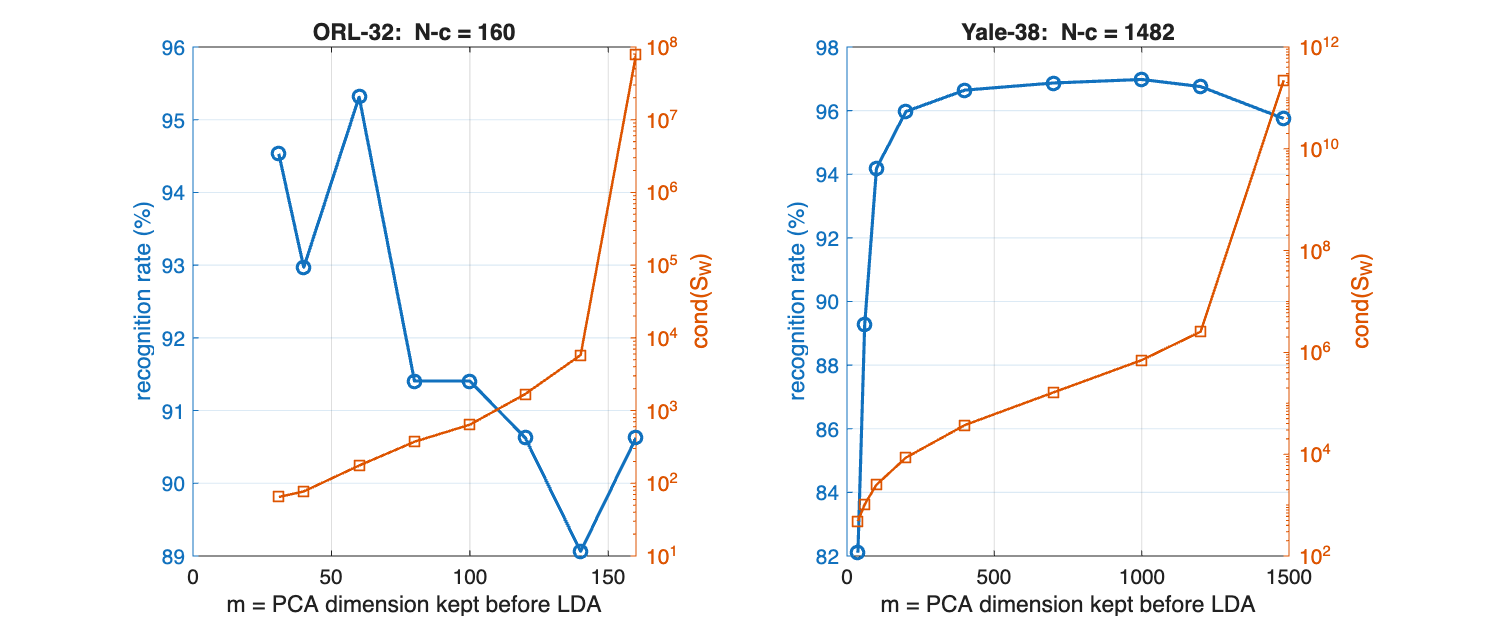
\includegraphics[width=0.95\textwidth]{figs/s9_m_sweep.png}
\caption{S9: recognition rate (left axis) and $\kappa(\Sw)$ on a log scale (right
axis) against $m$. The conditioning blow-up as $m\to N-c$ is the mechanism behind
the accuracy drop.}
\label{fig:msweep}
\end{figure}

\section{Sweeping the number of training images per subject}

\begin{table}[htbp]
\centering
\begin{tabular}{rrrrrr}
\toprule
$n_j$ & $N$ & $N-c$ & Correlation & Eigenfaces (best $k$) & \textbf{Fisherfaces} \\
\midrule
 2 &   76 &   38 & 26.6 & 19.9 & \textbf{43.0} \\
 3 &  114 &   76 & 29.9 & 22.2 & \textbf{51.5} \\
 5 &  190 &  152 & 42.4 & 34.3 & \textbf{69.6} \\
10 &  380 &  342 & 57.7 & 43.3 & \textbf{76.9} \\
20 &  760 &  722 & 72.1 & 55.7 & \textbf{89.4} \\
32 & 1216 & 1178 & 80.8 & 64.1 & \textbf{91.7} \\
40 & 1520 & 1482 & 82.7 & 67.3 & \textbf{94.2} \\
\bottomrule
\end{tabular}
\caption{Yale, random split, varying training images per subject. $m=N-c$ throughout.}
\label{tab:nsweep}
\end{table}

\begin{observation}
Fisherfaces beats Eigenfaces at \emph{every} training-set size, including $n_j=2$
where $\Sw$ gets only one degree of freedom per class ($43.0\%$ vs $19.9\%$). We
had half-expected Fisherfaces to lose at the smallest $n_j$, as it does on ORL. It
does not, and the reason is instructive: on Yale the nuisance (illumination) is so
dominant that even a badly estimated $\Sw$ points roughly in the right direction,
and suppressing it approximately is still far better than not suppressing it at
all. On ORL there is no such dominant nuisance to suppress, so a noisy $\Sw$ buys
nothing and the inversion only adds variance.

The relative advantage does shrink as data grows -- $2.16\times$ at $n_j=2$ down to
$1.40\times$ at $n_j=40$ -- which is the expected convergence: with enough data,
PCA's leading components eventually separate identity from lighting too.
\end{observation}

\begin{figure}[htbp]
\centering
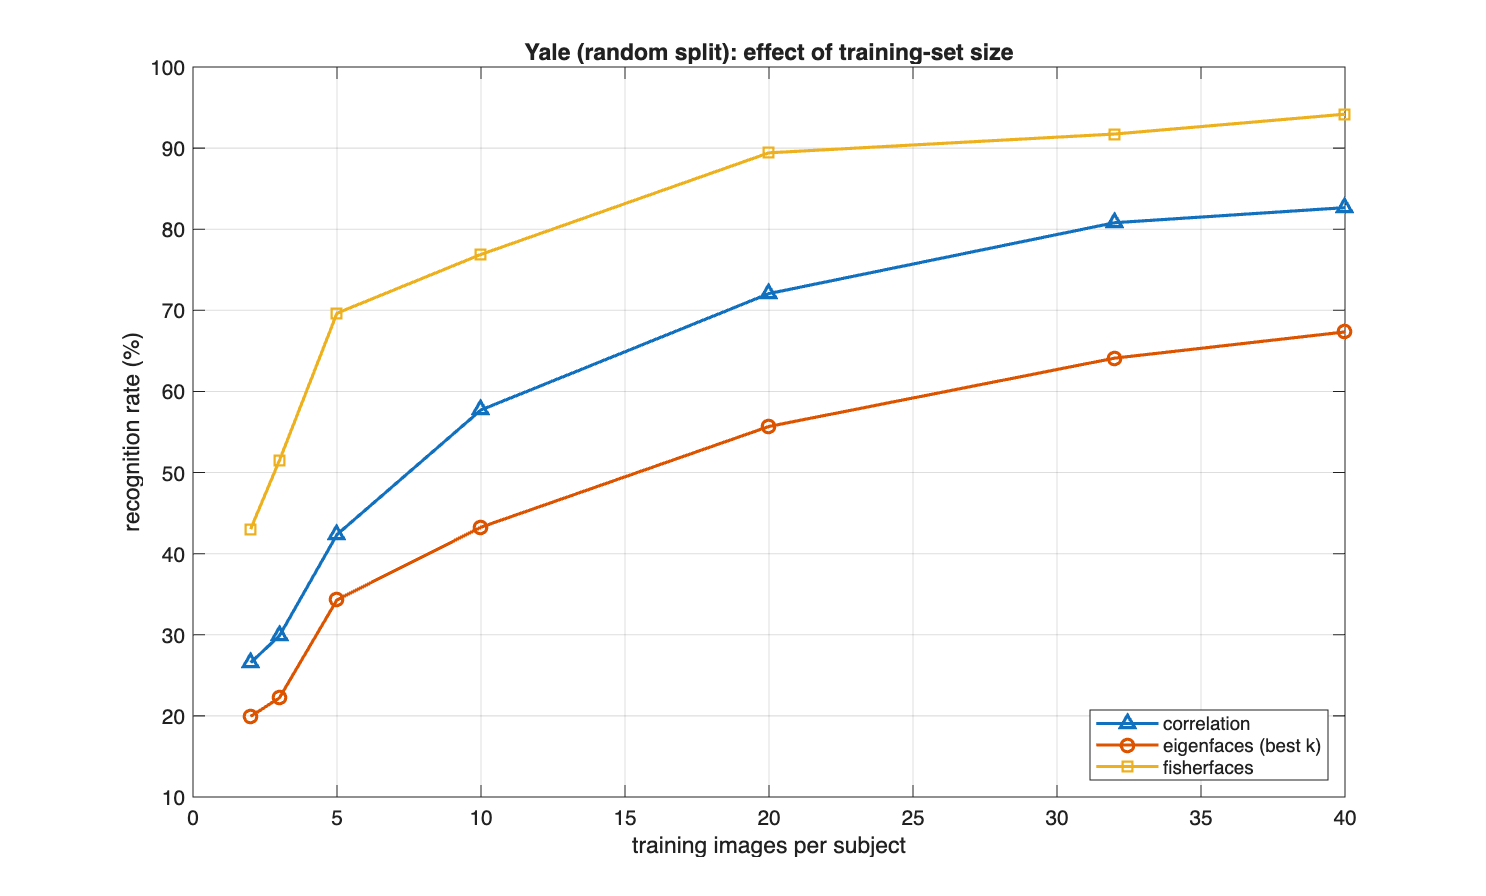
\includegraphics[width=0.75\textwidth]{figs/s10_n_sweep.png}
\caption{S10: all three methods improve with more training images, and the
Fisherfaces curve sits above the others throughout.}
\label{fig:nsweep}
\end{figure}

\section{What the basis images look like}

\begin{figure}[htbp]
\centering
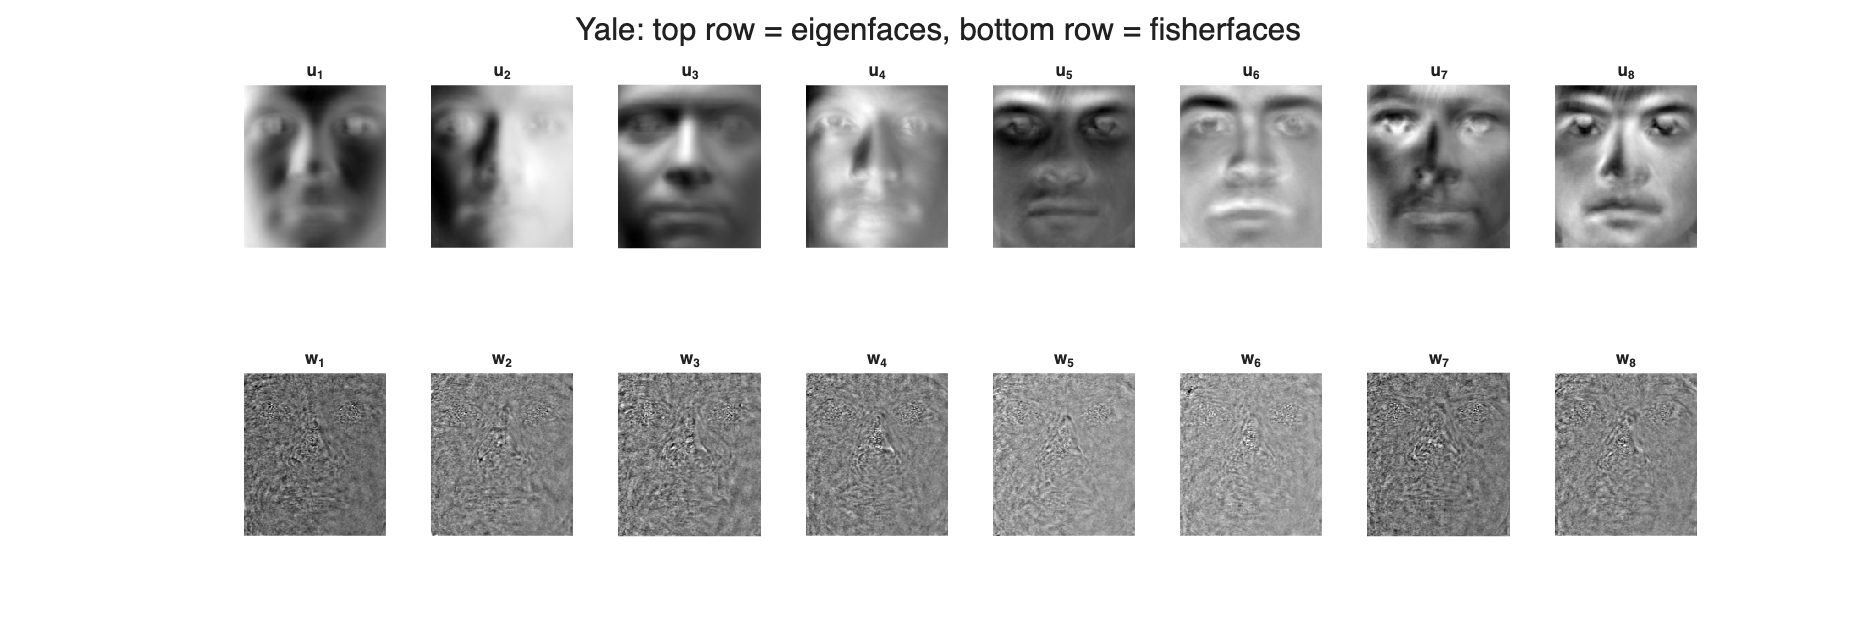
\includegraphics[width=0.93\textwidth]{figs/s11_yale_eigen_vs_fisher.png}
\caption{S11, Yale. Top row: the first eight eigenfaces. Bottom row: the first
eight Fisherfaces.}
\label{fig:basis}
\end{figure}

\begin{observation}
The two sets of images look completely different.

\textbf{Eigenfaces} are smooth and face-like, with broad soft gradients. They are
the directions of greatest variance, and on Yale the leading ones are dominated by
left--right and top--bottom lighting gradients --- you can practically read the
lamp position off the first few.

\textbf{Fisherfaces} are high-frequency, speckled, and much less recognisable as
faces. On ORL the leading eigenfaces instead show pose and expression changes,
since ORL has almost no lighting variation --- which is the same fact that makes
``drop the top 3'' help on Yale and hurt on ORL.
\end{observation}

\subsection{This is predicted, not just observed}

It would be weak to leave that as an impression. The high-frequency look of the
Fisherfaces is a \emph{consequence} of the whitening step, and the argument is
short.

A Fisherface is $w_l = R^{-1}z_l$, where $\Sw = R^{\!\top}R$. Work in the
eigenbasis of $\Sw$: if $\Sw q = \lambda q$, then applying $R^{-1}$ scales that
direction by $1/\sqrt{\lambda}$. So whitening \textbf{amplifies the
smallest-variance directions of $\Sw$ the most}. Now ask what those directions
look like:
\begin{itemize}[nosep]
\item $\Sw$'s \emph{large}-$\lambda$ directions are the ways one person's images
      differ most from each other --- broad shading, overall brightness, slight
      shifts. Those are \textbf{low spatial frequency}.
\item $\Sw$'s \emph{small}-$\lambda$ directions are where a person barely varies
      at all: fine detail, pixel-scale texture. Those are \textbf{high spatial
      frequency}.
\end{itemize}
Whitening divides by $\sqrt{\lambda}$, so it suppresses the first group and
inflates the second. A Fisherface therefore \emph{has} to come out
high-frequency. No experiment is needed to anticipate it.

\begin{observation}[Both halves of that argument, measured on ORL-32 (S14)]
Each basis image is Fourier-transformed; ``centroid'' is its power-weighted mean
radial spatial frequency and ``\%hi'' the share of power above a radial cutoff of
$0.15$.
\begin{center}
\begin{tabular}{lcc}
\toprule
mean over the first 10 & frequency centroid & \%\,power at high frequency \\
\midrule
eigenfaces   & $0.0306$ & $2.3\%$ \\
Fisherfaces  & $0.1178$ & $25.9\%$ \\
\midrule
ratio        & $\mathbf{3.85\times}$ & $11\times$ \\
\bottomrule
\end{tabular}
\end{center}
So ``they look noisy'' is worth $3.85\times$ in frequency centroid and an
eleven-fold increase in high-frequency power share.

And the mechanism itself checks out. Measuring the frequency centroid of $\Sw$'s
own eigen-directions, ordered by eigenvalue:
\begin{center}
\begin{tabular}{lcccc}
\toprule
rank of $\lambda$ & 1 & 5 & 20 & 80 \\
$\lambda$         & $9.99\times10^{7}$ & $4.14\times10^{7}$ & $1.18\times10^{7}$ & $3.27\times10^{6}$ \\
centroid          & $0.0226$ & $0.0378$ & $0.0834$ & $0.1673$ \\
\bottomrule
\end{tabular}
\end{center}
Large eigenvalue means smooth, small eigenvalue means fine detail, exactly as the
argument requires. And since
$\lambda_{\max}/\lambda_{\min} = 7.85\times10^{7}$ here, whitening amplifies the
finest direction by about $\sqrt{7.85\times10^{7}} \approx 8860$ relative to the
smoothest.
\end{observation}

\begin{gotcha}
The trend is not perfectly monotonic at the very tail: rank $160$ (the last, with
$\lambda = 1.27$) has centroid $0.1166$, slightly \emph{below} rank $80$. That is
not a counterexample to the argument --- it is the zero-slack problem of
Section~\ref{sec:zeroslack} again. At $m=N-c$ the last directions of $\Sw$ are
estimated from almost no data, so their frequency content is as noisy as
everything else about them. The clean part of the trend is ranks 1--80.
\end{gotcha}

\paragraph{What genuinely does need the pictures.} The argument above predicts
\emph{that} Fisherfaces are high-frequency and \emph{that} eigenfaces are smooth.
It does not predict \emph{where} on the face the discriminative energy lands
(around the eyes and nose bridge, as the figures show), nor whether a given
database's leading eigenfaces will encode lighting or pose --- that depends on
which nuisance dominates, which is a property of the data and not of the method.
Those two things are what the figures are for.



\begin{figure}[htbp]
\centering
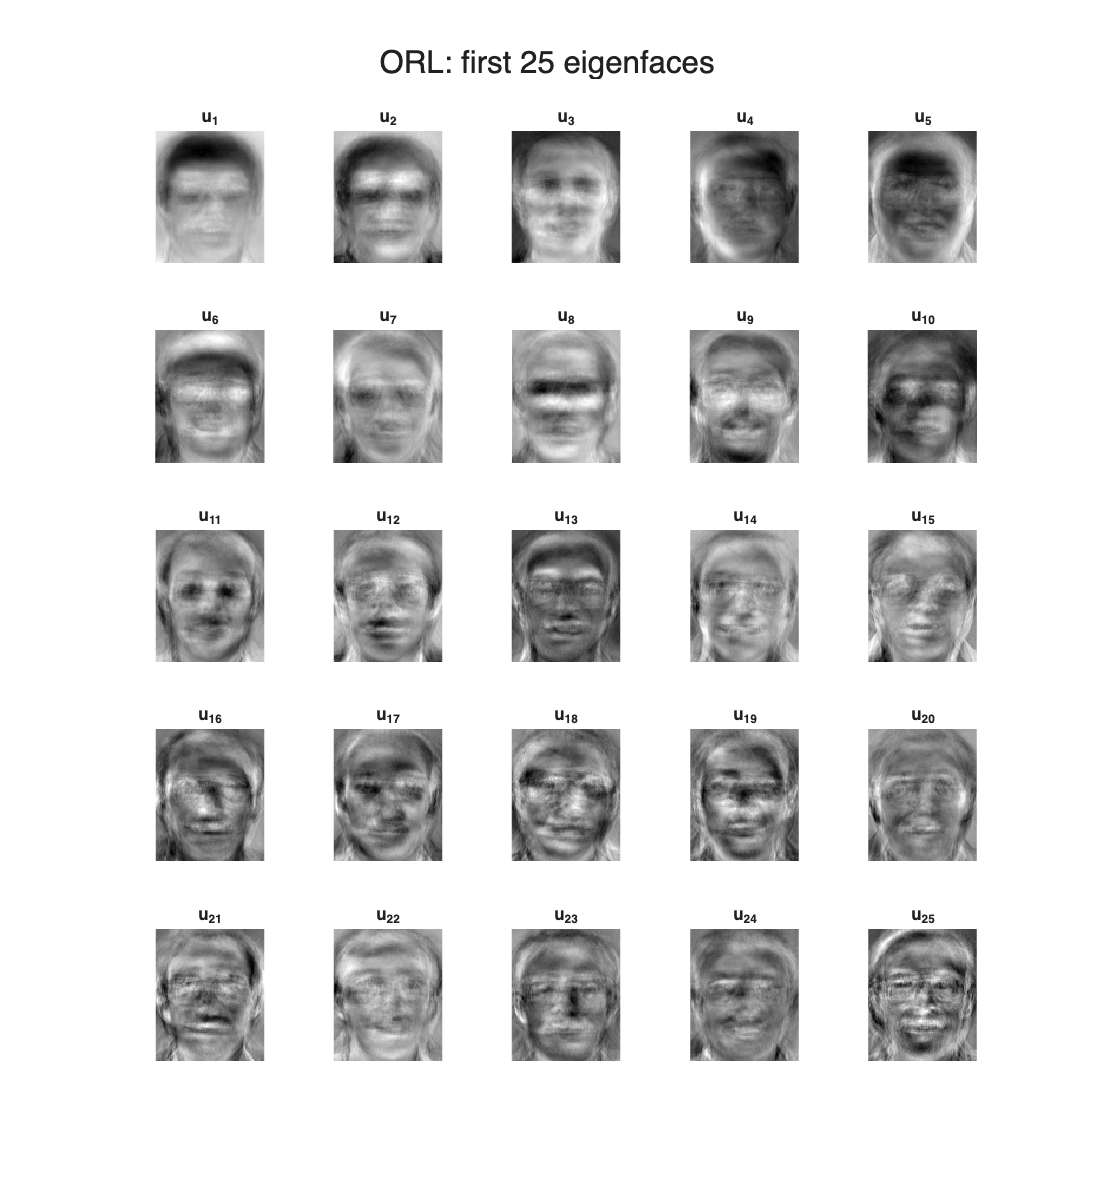
\includegraphics[width=0.42\textwidth]{figs/s11_orl_eigenfaces.png}
\hfill
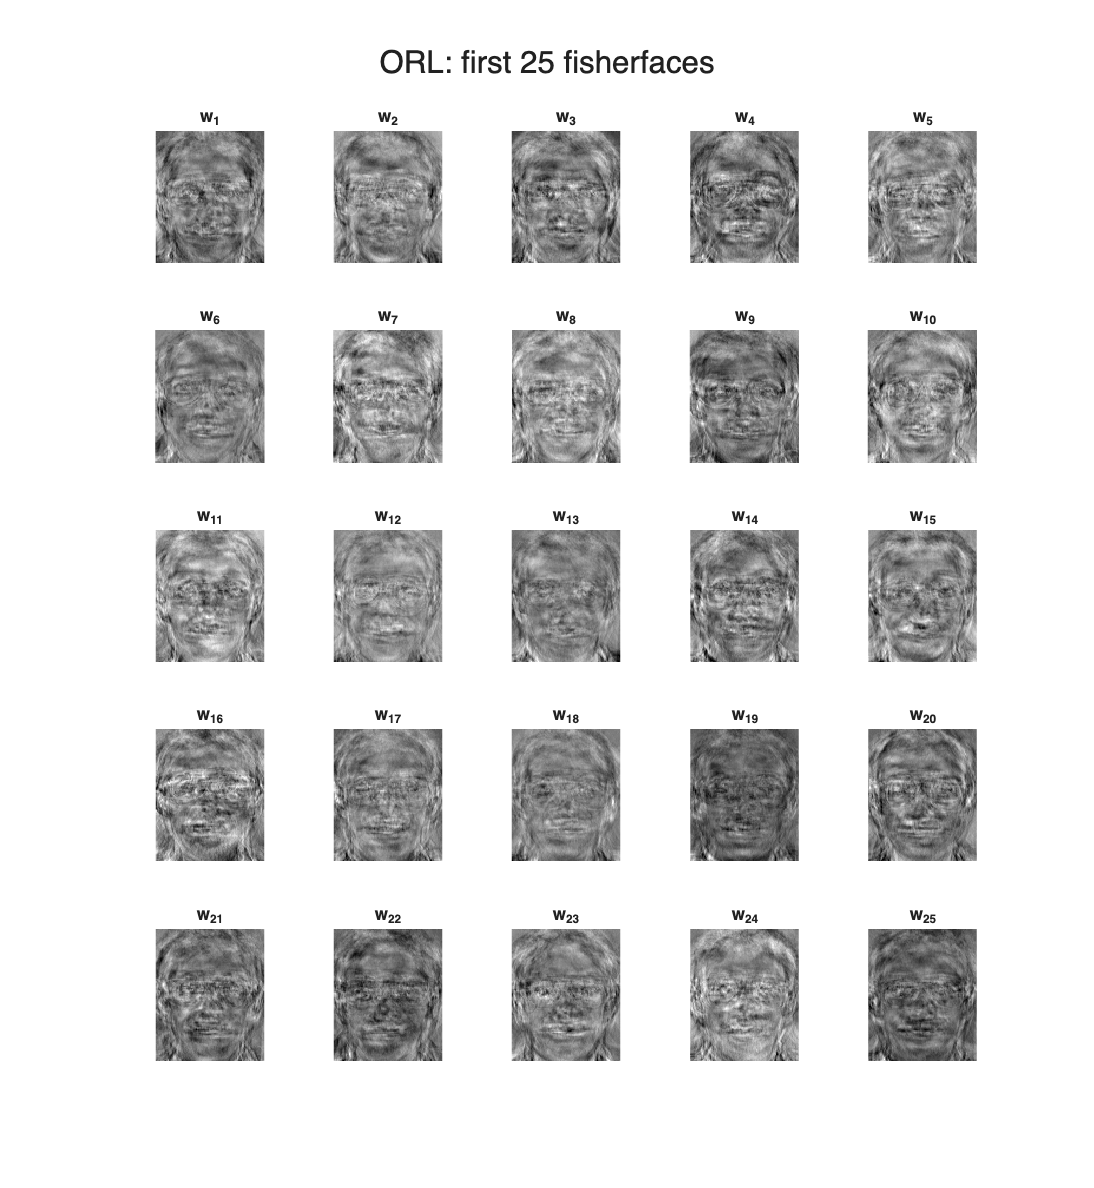
\includegraphics[width=0.42\textwidth]{figs/s11_orl_fisherfaces.png}
\caption{S11, ORL. Left: the first 25 eigenfaces. Right: the first 25 Fisherfaces
(there are exactly $c-1=31$ in total). The same contrast as Figure~\ref{fig:basis}
appears on the second database: eigenfaces are smooth and face-like, Fisherfaces
are high-frequency. ORL has little lighting variation, so its leading eigenfaces
show pose and expression changes rather than lighting gradients -- which is why
discarding them hurts here and helps on Yale.}
\label{fig:orlbasis}
\end{figure}

\begin{figure}[htbp]
\centering
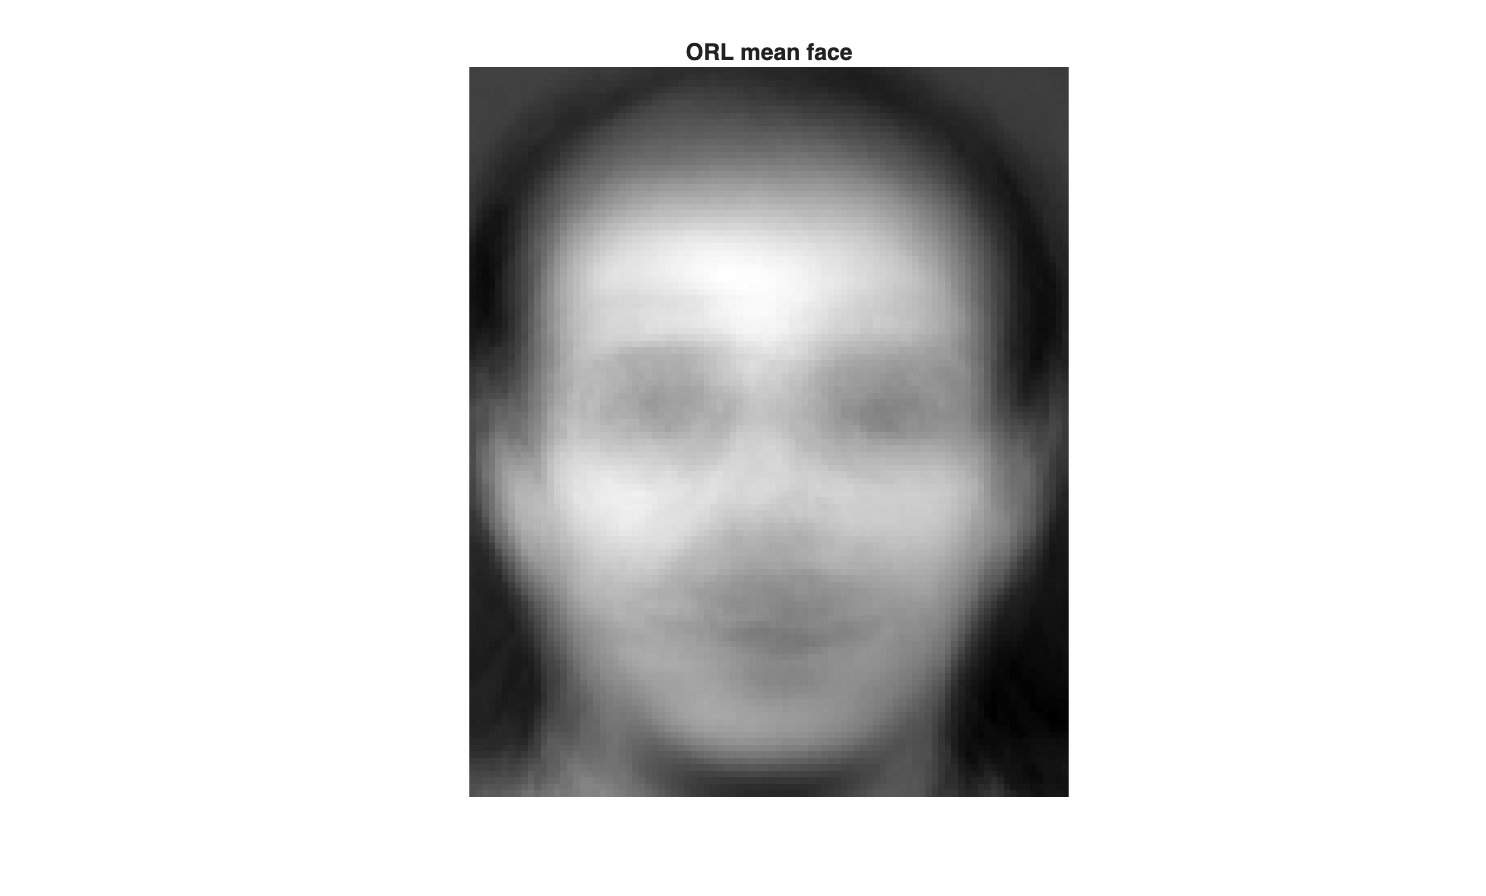
\includegraphics[width=0.30\textwidth]{figs/s11_orl_meanface.png}
\caption{S11: the ORL mean face $\bar{x}$, subtracted from every image before PCA. It
is recognisably a face because it averages what all the subjects have in common;
PCA then describes how individuals deviate from it.}
\label{fig:meanface}
\end{figure}

\begin{figure}[htbp]
\centering
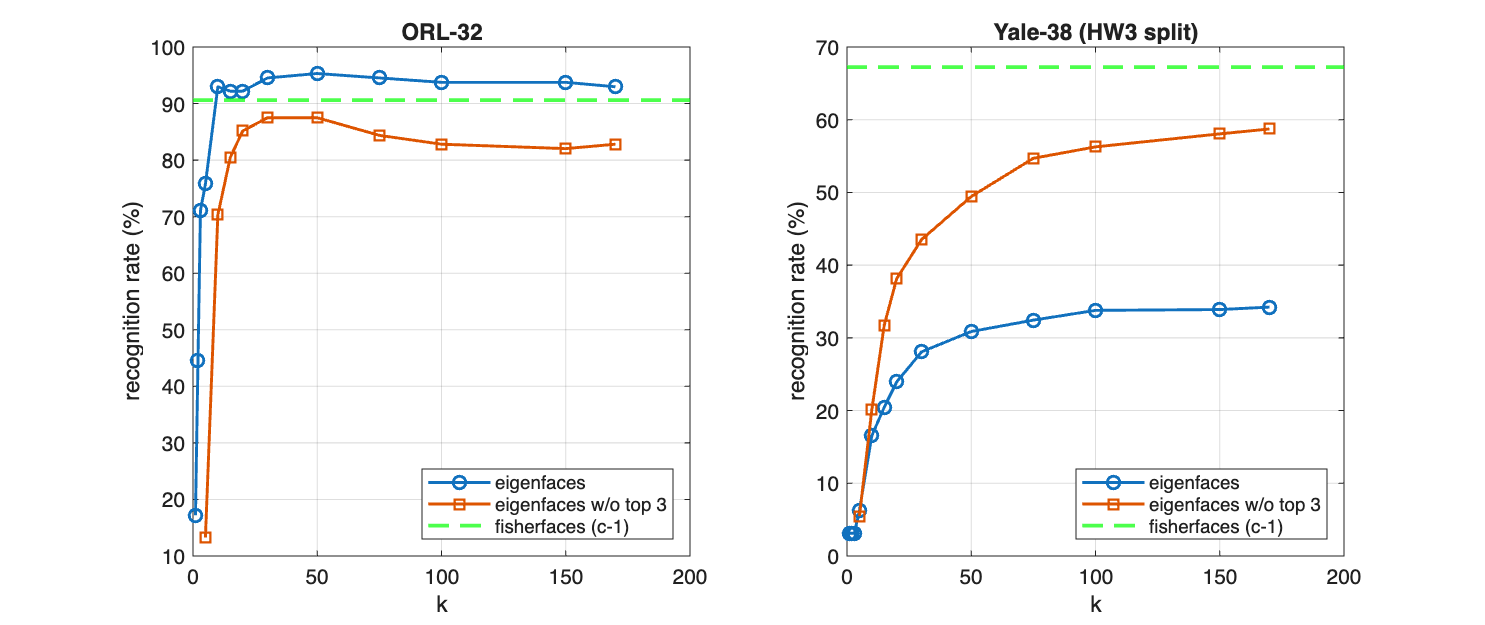
\includegraphics[width=0.8\textwidth]{figs/s11_rate_curves.png}
\caption{S11: recognition rate against $k$ for the two Eigenfaces variants, with
the Fisherfaces result (a single number, since it always uses $c-1$ features) drawn
as a dashed line. Left: ORL-32, where Fisherfaces sits below the Eigenfaces curve.
Right: Yale-38, where it sits well above both.}
\label{fig:curves}
\end{figure}

\begin{figure}[htbp]
\centering
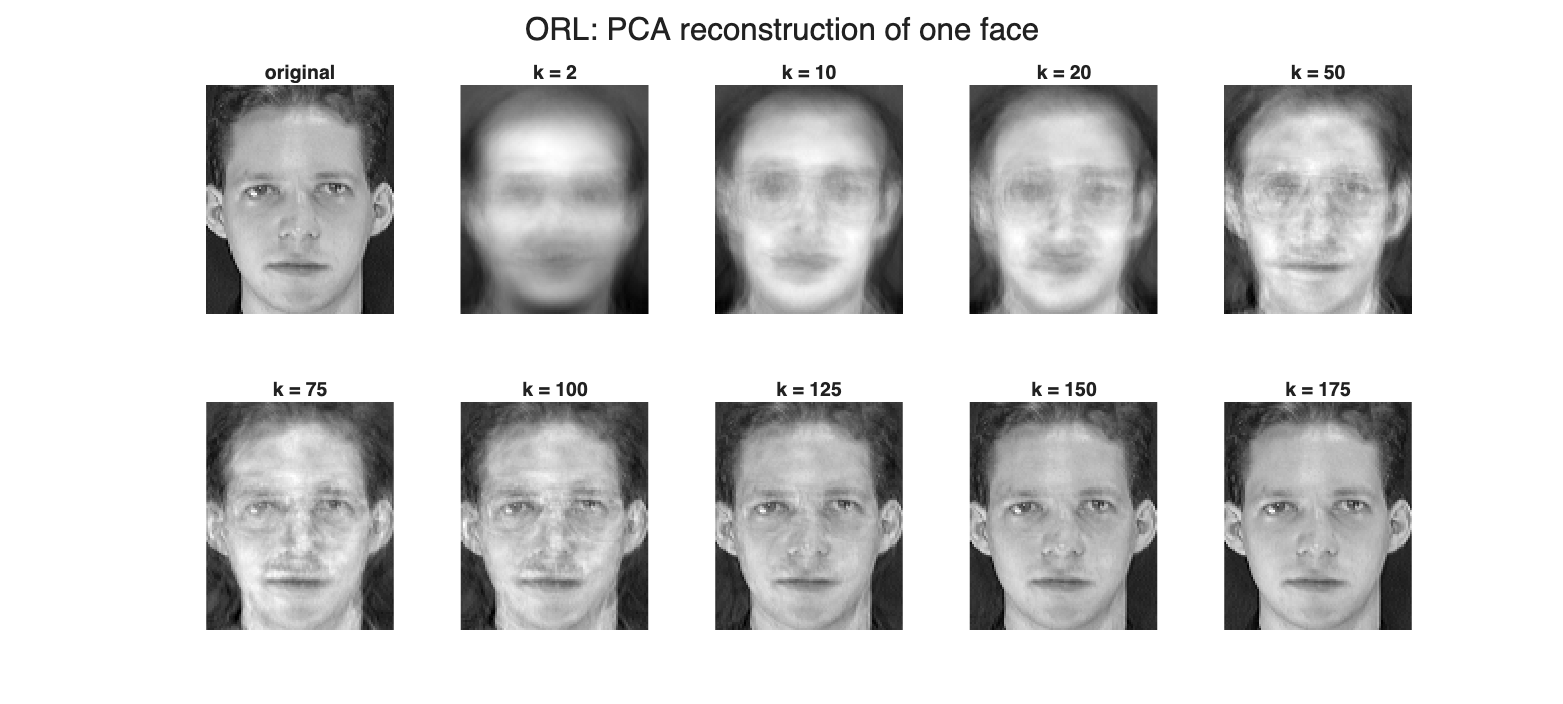
\includegraphics[width=0.92\textwidth]{figs/s11_orl_reconstruction.png}
\caption{S11: PCA reconstruction of one ORL face as $k$ grows, the visual
counterpart of Theorem~\ref{thm:recon}. By $k=50$ the identity is clear; the
remaining components add fine texture.}
\label{fig:recon}
\end{figure}

\section{Summary of what we verified}

\begin{center}
\begin{tabular}{lll}
\toprule
Check & Where & Result \\
\midrule
HW3 eigenfaces numbers reproduced   & S3/S4 & exact to all printed digits \\
$E_k=\sum_{i>k}\lambda_i$           & S3/S4 & agrees to 4 decimals \\
$\St=\Sb+\Sw$                       & S5--S8 & $\le 8.6\times10^{-16}$ relative \\
$\rank(\Sw)\le N-c$                 & S5 & $1482 = 1482$, bound met \\
no duplicate training images        & S5 & $0$ pairs (after cleaning) \\
our solver vs \texttt{eig(Sb,Sw,'chol')} & S6--S8 & $\le 7.8\times10^{-16}$ relative \\
eigenfaces orthonormal              & S12(a) & $\|V^{\!\top} V-I\|_F=9.1\times10^{-14}$ \\
\texttt{eig} route vs \texttt{svd} route & S12(b) & $|u^{\!\top} u'|=1.000000$ for top 10 \\
Fisherfaces $\Sw$-orthogonal        & S12(c) & off-diagonal $3.8\times10^{-13}$ \\
Fisherfaces \emph{not} Euclidean-orthogonal & S12(c) & off-diagonal $0.499$ \\
$\rank(\Sb)=c-1$                    & S12(d) & $31 = 31$ \\
$\Sw$ singular once $m>N-c$         & S13 & \texttt{chol} fails at $m=N-1$, $\kappa\sim10^{18}$--$10^{22}$ \\
closed-form $w$ maximises $J$       & S1 & beats a 6283-direction grid search \\
LDA error vs Bayes error            & S1 & $1.70\%$ vs $2.28\%$ theoretical \\
\bottomrule
\end{tabular}
\end{center}

\section{Conclusions}

\begin{enumerate}[leftmargin=*]
\item \textbf{The paper's central claim holds.} Where the within-class nuisance is
  large and structured -- illumination on Yale -- supervised LDA beats unsupervised
  PCA decisively, $67.2\%$ vs $34.2\%$ and $97.1\%$ vs $70.0\%$.
\item \textbf{It is a claim about nuisance structure, not about LDA being better.}
  On ORL, where variation is pose and expression and only six images per person are
  available, Fisherfaces \emph{loses} to Eigenfaces. The deciding quantity is the
  per-class degrees of freedom $n_j-1$ available to estimate $\Sw$.
\item \textbf{The $m=N-c$ prescription is the weakest part of the recipe.} It is
  the largest $m$ making $\Sw$ invertible, but it is the \emph{worst-conditioned}
  such choice, and on both databases a smaller $m$ does better ($95.3$ vs $90.6$ on
  ORL, $97.0$ vs $95.7$ on Yale). On one split it does not even deliver the
  invertibility it was chosen for.
\item \textbf{Dropping the first three components is a weaker version of the same
  idea.} It hard-codes the assumption that the nuisance is a fixed 3-D subspace;
  LDA learns the nuisance from labels instead, and does better
  ($67.2$ vs $58.7$, $97.1$ vs $89.0$).
\item \textbf{Experimental protocol mattered as much as the algorithm.} The
  lexicographic Yale split suppressed every method's score by roughly a factor of
  two, and a duplicated file in the database was visible as a one-unit rank
  deficiency. Both were found by checking numbers against theory rather than by
  looking at recognition rates.
\end{enumerate}

\part{Question bank}

Short answers to the questions this project most invites. Each points back to the
section with the full argument.

\section{Theory}

\begin{description}[leftmargin=*,style=nextline]

\item[Why subtract the mean before PCA?]
PCA finds directions of maximum \emph{variance}, which is spread about the centre.
Without centring, the first component points at the mean face itself -- the
direction in which the raw vectors are largest -- which describes what faces have
in common rather than how they differ. (Section~\ref{sec:centre})

\item[Why does the $L=X^{\!\top}\!X$ trick work?]
If $Lw=\lambda w$ then $XX^{\!\top}(Xw)=X(X^{\!\top}\!Xw)=\lambda(Xw)$, so $Xw$ is an
eigenvector of $XX^{\!\top}$ with the same eigenvalue. We get the eigenvectors of a
$32256\times32256$ matrix from a $1520\times1520$ one. (Theorem~\ref{thm:gram})

\item[When is that trick a bad idea?]
When $N > d$. It trades an $O(d^3)$ problem for an $O(N^3)$ one, so it only helps
while $N\ll d$. On MNIST ($d=784$, $N=60000$) it would be far slower than forming
the covariance directly.

\item[Why must you renormalise $Xw$?]
$\|Xw\|=\sqrt{\lambda}$, not $1$. Without renormalising, $\hat{V}_k^{\!\top}\hat{V}_k\ne I$, the
reconstruction formula stops being an orthogonal projection, and
Theorem~\ref{thm:recon} fails.

\item[How many eigenfaces can you possibly get from $N$ images?]
At most $N-1$. The mean-subtracted columns satisfy $\sum_j a_j = 0$, one linear
dependency, so $\rank(A)\le N-1$. (Corollary~\ref{cor:rank})

\item[What exactly is the reconstruction error for $k$ components?]
The sum of the discarded eigenvalues, $\sum_{i>k}\lambda_i$. Proved by expanding in
the eigenbasis and applying Pythagoras twice. (Theorem~\ref{thm:recon})

\item[Why does dropping the first three eigenfaces help on Yale?]
For a convex Lambertian surface with no shadowing, every image of one face under
any lighting is $B\mathbf{s}$ with $B\in\R^{d\times3}$, so lighting variation spans
only a 3-D subspace. That variation is larger than the differences between people,
so PCA spends its leading components on it. (Theorem~\ref{thm:cone})

\item[Then why does the same trick hurt on ORL?]
ORL has almost no lighting variation; it varies by pose and expression. There the
leading components carry real identity information, so discarding them destroys
signal. The trick is a targeted fix for a specific nuisance, not a general
improvement.

\item[Derive the two-class Fisher direction.]
Maximise $J(w)=w^{\!\top}\Sb w/w^{\!\top}\Sw w$. It is scale-invariant, so fix
$w^{\!\top}\Sw w=1$ and use a Lagrange multiplier: $\Sb w=\lambda\Sw w$. For two
classes $\Sb=\frac{n_1n_2}{n}\delta\delta^{\!\top}$ is rank one with
$\delta=\mu_1-\mu_2$; substituting and cancelling scalars gives
$w\propto\Sw^{-1}(\mu_1-\mu_2)$. (Section~\ref{sec:twoclass})

\item[What is a generalised eigenvalue problem, and why is ours a nice one?]
A pencil $(A,B)$ with $Aw=\lambda Bw$; $B=I$ gives the ordinary problem. Ours is a
\emph{symmetric-definite} pencil ($\Sb$ symmetric PSD, $\Sw$ symmetric PD), which
is as well behaved as the ordinary symmetric case: Theorem~\ref{thm:simdiag} gives
a single $W$ with $W^{\!\top}\Sw W=I$ and $W^{\!\top}\Sb W=\Lambda$ simultaneously.
Real eigenvalues, $\Sw$-orthogonal eigenvectors and the $c-1$ ceiling are all
corollaries of that one theorem. See Section~\ref{sec:gevp}.

\item[What happens to the pencil when $\Sw$ is singular?]
Two different things. If $\Sw w=0$ but $\Sb w\neq0$ the eigenvalue is
\emph{infinite} --- a direction with zero within-class spread and separated means,
which is exactly what null-space LDA hunts for. If instead $\Sb w=\Sw w=0$ then
$\Sb w=\lambda\Sw w$ holds for \emph{every} $\lambda$: the pencil is
\emph{singular} and its eigenvalues are undefined. Past $m=N-c$ we are in the
second case, so the real objection to a large $m$ is not that $\Sw^{-1}$ fails to
exist but that the problem stops having a unique answer.

\item[Why exactly $c-1$ non-zero eigenvalues?]
$M = R^{-\top}\Sb R^{-1}$ is a congruence of $\Sb$ by an invertible matrix, and
congruence preserves rank, so $\rank(M)=\rank(\Sb)\le c-1$. Measured on ORL-32
(S12(e)): $\lambda_{31}=7.47$ and $\lambda_{32}=2.1\times10^{-12}$ --- a cliff of
twelve orders of magnitude exactly at $l=c-1$.

\item[What is the eigenvalue $\lambda$, physically?]
Multiplying $\Sb w=\lambda\Sw w$ on the left by $w^{\!\top}$ gives
$\lambda = w^{\!\top}\Sb w / w^{\!\top}\Sw w = J(w)$. The eigenvalue \emph{is} the value
of the Fisher criterion for that direction, which is why we sort descending.

\item[Why is $\|w\|$ irrelevant, and when does it suddenly matter?]
$J(\alpha w)=J(w)$, so the criterion fixes only a direction. But
nearest-neighbour \emph{distances} depend on the relative scaling of the axes, so
once we classify we must pick a convention. We normalise each Fisherface to unit
norm and say so.

\item[Prove $\St=\Sb+\Sw$.]
Split $x-\bar{x}=(x-\mu_j)+(\mu_j-\bar{x})$, expand the outer product, and note the cross
terms vanish because $\sum_{x\in j}(x-\mu_j)=0$ by definition of the class mean.
(Theorem~\ref{thm:decomp})

\item[Why at most $c-1$ Fisherfaces?]
$\Sb$ is spanned by the $c$ vectors $\mu_j-\bar{x}$, which obey the one relation
$\sum_j n_j(\mu_j-\bar{x})=0$, so $\rank(\Sb)\le c-1$. Any $w$ in the null space of
$\Sb$ gives $\lambda=0$. (Theorem~\ref{thm:rankSb})

\item[Why is $\rank(\Sw)\le N-c$?]
$\Sw=A_WA_W^{\!\top}$ where $A_W$ holds the within-class-centred images. Each class's
$n_j$ columns sum to zero, so contribute at most $n_j-1$ independent directions;
summing, $\sum_j(n_j-1)=N-c$. (Theorem~\ref{thm:rankSw})

\item[Is that bound always attained?]
No, it is an upper bound. We measured $1481$ instead of $1482$ on Yale and traced
it to a duplicated image file, which is an exact linear dependency. After removing
it the bound is met exactly.

\item[Are Fisherfaces orthogonal?]
Not in the Euclidean sense. They satisfy $w_l^{\!\top}\Sw w_{l'}=\delta_{ij}$, i.e.\ they
are orthonormal in the inner product defined by $\Sw$. We measured the Euclidean
Gram matrix to have about half its energy off the diagonal, while $W^{\!\top}\Sw W$ is
diagonal to $10^{-13}$. Eigenfaces \emph{are} orthonormal; Fisherfaces are not.

\item[Is the set of Fisherfaces unique?]
No. $J(WM)=J(W)$ for any invertible $M$, so LDA determines a subspace, not a
basis or a scaling. Different correct implementations can produce different-looking
Fisherface images. (Theorem~\ref{thm:invariance})

\item[Where do the class labels come from?]
From the directory structure. Both databases ship one folder per person ---
\texttt{s1}\ldots\texttt{s40} for ORL, \texttt{yaleB01}\ldots\texttt{yaleB39} for
Yale --- so the folder an image sits in \emph{is} its ground-truth identity. In
the loader this is the single line \texttt{ytr(a) = p}, where \texttt{p} is the
subject index. Nobody labels anything by hand; the supervision was free, baked
into how the data was distributed.

\item[If Eigenfaces is ``unsupervised'', how does it recognise anyone?]
Because ``unsupervised'' describes only how the \emph{subspace} is built, not the
whole pipeline. PCA chooses its directions without ever seeing a label --- in our
code \texttt{doPCA(imgs)} has no label argument at all, so it \emph{cannot} see
them --- but the nearest-neighbour step that follows does use the training labels,
since it answers ``whose face is the closest training image?''. So:
\begin{center}
\begin{tabular}{lcc}
\toprule
 & subspace uses labels? & classifier uses labels? \\
\midrule
Eigenfaces  & no  & yes \\
Fisherfaces & yes & yes \\
\bottomrule
\end{tabular}
\end{center}
Both need labels to name a person. The difference is whether the labels shaped the
projection. Test labels (\texttt{yte}) are used only to score correctness --- using
them to classify would be cheating.

\item[When is LDA actually optimal?]
When the classes are Gaussian with a \emph{shared} covariance and equal priors, the
Bayes-optimal boundary is linear and LDA finds it. Our toy experiment confirms it:
measured error $1.70\%$ against a theoretical Bayes error of $2.28\%$. With
strongly unequal covariances the optimal boundary is quadratic and LDA is no longer
optimal.

\end{description}

\section{The Fisherfaces construction}

\begin{description}[leftmargin=*,style=nextline]

\item[Why is a PCA stage needed at all?]
$\Sw$ is $d\times d$ ($8.3$~GB for Yale) \emph{and} singular, since
$\rank(\Sw)\le N-c=1482 \ll d=32256$. PCA fixes both: it shrinks the matrix and
removes the guaranteed null space. The PCA stage is a workaround for $d\gg N$, not
a part of LDA.

\item[Why exactly $m=N-c$?]
It is the largest $m$ for which the projected $\Sw$ is non-singular. Above it,
rank is still capped at $N-c$ so $\Sw$ stays singular; at or below it, $\Sw$ is
generically full rank.

\item[So is $m=N-c$ the best choice?]
No, and this is the most interesting result we have. ``Invertible'' is not ``well
conditioned'': at $m=N-c$ the rank equals the dimension exactly, with no slack, so
the smallest eigenvalues of $\Sw$ are estimation noise and $\Sw^{-1}$ amplifies
them. Our sweep finds a clearly better $m$ on both databases.
(Section~\ref{sec:msweep})

\item[Why PCA-then-LDA rather than just regularising $\Sw$?]
Three reasons, in order of honesty. It is the paper's method and this is a
reproduction. It fixes \emph{both} of $\Sw$'s defects --- size and rank --- whereas
a ridge in pixel space fixes only the rank and still leaves an 8.3~GB matrix. And
it has no free parameter, so the result needs no validation set. Section S13
measures the alternatives: tuning $m$, or ridge with a well-chosen $\varepsilon$,
both beat $m=N-c$ (Yale $95.5 \to 97.3$ or $97.9$), so the recipe's merit is that
it is principled, not that it wins. See Section~\ref{sec:alternatives}.

\item[What happens if you keep more than $N-c$ components?]
$\Sw$ becomes singular and \texttt{chol} fails outright. We measured it: at
$m=N-1$, $\kappa(\Sw)$ is $8.3\times10^{17}$ on ORL and $9.8\times10^{21}$ on
Yale, and the factorisation is refused on both. This is the rank theorem
$\rank(\Sw)\le N-c$ appearing as a crash rather than an inequality.

\item[How exactly does the nearest-neighbour step work, and when does it converge?]
It never converges, because it never iterates. There is no training phase at all:
we store the projected training vectors and their labels, and to classify a probe
we project it, compute $N$ squared distances, and take the \texttt{argmin}. Fixed
work, no loop, no tolerance, no per-class state. The question usually comes from
confusing 1-NN with $k$-means, which does alternate assignment and update steps
until convergence --- but that is unsupervised clustering, not this. Nothing in
this project is trained iteratively: PCA and LDA are both closed-form
eigenproblems. See Section~\ref{sec:nn}.

\item[Which route would you defend for solving $\Sb w = \lambda \Sw w$?]
Cholesky whitening --- but not on accuracy grounds. We measured six routes and
all six give the same recognition rate and a subspace differing by $0.00^\circ$.
The case is: it needs only two one-line facts (SPD $\Rightarrow$ Cholesky exists;
symmetric $\Rightarrow$ real eigenvalues and orthogonal eigenvectors), every step
is visible rather than hidden in a library call, it was the fastest route
measured, its guarantees hold by construction rather than by luck, and its
\emph{failure} is informative --- \texttt{chol} refusing is how we detected
$\rank(\Sw)\le N-c$ empirically. See Section~\ref{sec:routes}.

\item[Did the non-symmetric route actually produce complex eigenvalues?]
Yes, but only about $8\times10^{-9}$ in magnitude --- negligible, and the final
answer was unchanged. The theoretical warning is real; at
$\kappa(\Sw)=4\times10^{11}$ double precision still copes. It would bite nearer
$\kappa\sim10^{16}$. Claiming Cholesky was \emph{necessary} here would be
overstating it.

\item[Why not just use $\Sw^{-1}\Sb$ and \texttt{eig}?]
$\Sw^{-1}\Sb$ is not symmetric, so a general eigensolver is used and round-off can
return complex eigenvalues and non-orthogonal eigenvectors. It also forms
$\Sw^{-1}$ explicitly, which is the worst thing to do to an ill-conditioned matrix.

\item[What does Cholesky whitening do?]
Writes $\Sw=R^{\!\top} R$ and substitutes $w=R^{-1}z$, turning the generalised problem
into the \emph{symmetric} ordinary problem $R^{-\top}\Sb R^{-1}z=\lambda z$.
Symmetric eigensolvers guarantee real eigenvalues, orthogonal eigenvectors and
backward stability. Conceptually: whiten with $\Sw$, then do PCA on the class
means. (Section~\ref{sec:solve})

\item[Why re-symmetrise with \texttt{(M+M')/2}?]
Floating-point addition is not associative, so accumulating outer products in a
loop leaves the result differing from its transpose by about $10^{-16}$. \texttt{chol}
and symmetric \texttt{eig} read one triangle and assume the other matches, so the
asymmetry can mislead them. The triangular solves reintroduce it, so we do it
twice.

\item[What if \texttt{chol} fails?]
Its second output \texttt{p} is non-zero. We add a ridge
$\varepsilon = 10^{-6}\tr(\Sw)/m$ and retry, and we log that it happened. The
scaling by $\tr(\Sw)/m$ (the mean eigenvalue) makes $\varepsilon$ comparable to
$\Sw$'s own magnitude, which a bare constant would not be.

\item[Is the naive $\Sw^{-1}\Sb$ route actually bad on \emph{your} data?]
No, and we measured rather than assumed. On Yale at $\kappa(\Sw)=4.19\times10^{11}$
it returns the same $95.5\%$, a subspace agreeing with Cholesky to $0.00^\circ$,
and imaginary parts of only $8.4\times10^{-9}$. It survives because we keep only
the top $c-1$ eigenvalues, which are separated by orders of magnitude
($1.49\times10^{7}$, $7.15\times10^{4}$, $1.81\times10^{4}$), and eigenvector
error grows as those gaps close. We still prefer Cholesky for three reasons that
are not about accuracy here: it is about $2.7\times$ faster (ratio stable over
three runs at $2.58$--$2.81$, though the absolute seconds are not),
it needs no \texttt{real()}/re-sort cleanup, and its correctness does not depend
on the gaps being large. (Section~\ref{sec:naive})

\item[Could you use the lower-triangular Cholesky $\Sw=LL^{\!\top}$ instead?]
Yes, and it gives the \emph{identical} matrix. With $L=R^{\!\top}$ and the
substitution $w=L^{-\top}z$ you get $L^{-1}\Sb L^{-\top}z = \lambda z$, and
$L^{-1}\Sb L^{-\top} = R^{-\top}\Sb R^{-1}$, so same eigenvalues, same
Fisherfaces. The choice is purely which form the library hands you: MATLAB's
\texttt{chol(Sw)} returns the upper factor $R$ with \texttt{R'*R == Sw}, so the
code is written that way; \texttt{chol(Sw,'lower')} would work with one line
changed. Both are triangular solves --- neither forms an inverse.
(Section~\ref{sec:solve})

\item[Why report Eigenfaces at $k=c-1$ as well as at its best $k$?]
Fisherfaces always uses exactly $c-1$ features. Comparing it against Eigenfaces
using $170$ features is not like-for-like, so we report the matched-dimension case
too. It is the fairer comparison and it flatters Fisherfaces further.

\end{description}

\section{Code details}

\begin{description}[leftmargin=*,style=nextline]

\item[Why \texttt{double(imread(...))}?]
\texttt{imread} gives \texttt{uint8}. MATLAB's \texttt{uint8} arithmetic saturates
at $0$ and $255$ and rounds, so subtracting the mean would clip every negative
value to zero and silently destroy the data.

\item[Why sort the eigenvalues at all?]
\texttt{eig} returns them ascending, so without sorting we would keep the
\emph{least} informative directions. There is no error -- just chance-level
recognition.

\item[Why divide the eigenvalues by $M$?]
We diagonalise $L=X^{\!\top}\!X$ but the theory is about $C=\frac1N XX^{\!\top}$. Their
non-zero eigenvalues are equal, so the only difference is the $\frac1N$. Without
the division the reconstruction identity is wrong by a factor of $N$ -- and the
recognition rates are unaffected, which is what makes the bug hard to spot.

\item[Why compare $|u_1^{\!\top} u_2|$ rather than $\|u_1-u_2\|$?]
Eigenvector signs are arbitrary: $-u$ is as valid as $u$. Two correct programs can
return negated eigenfaces, so only the absolute inner product is meaningful.

\item[Why preallocate instead of \texttt{X = [X, im(:)]}?]
Growing an array reallocates and copies the whole thing every iteration. For Yale
that is 1520 copies of a 392~MB matrix. We count the files first, then fill a
preallocated array.

\item[Why build ORL paths by index rather than globbing \texttt{s*}?]
The \texttt{ORL/} directory contains a stray empty folder named \texttt{sed}, so
\texttt{dir('ORL/s*')} returns 41 entries and a glob-based loader would try to read
images from it. Constructing \texttt{['s' num2str(p)]} for $p=1\ldots40$ never sees
it.

\item[Why list the Yale directory instead of building names by index?]
\texttt{yaleB14} does not exist, so the names are not a contiguous numeric range
and index construction would fail on the gap.

\item[What is the difference between \texttt{mean(X,1)} and \texttt{mean(X,2)}?]
\texttt{mean(X,2)} averages across columns, giving the $d\times1$ \textbf{mean
face}. \texttt{mean(X,1)} averages down each column, giving a $1\times N$ row of
\textbf{per-image brightnesses}. Neither errors if confused.

\item[Why does \texttt{normCols} make nearest neighbour a correlation classifier?]
For zero-mean unit-norm $a,b$: $\|a-b\|^2 = 2-2a^{\!\top} b$. Minimising distance is
therefore exactly maximising correlation.

\item[Why squared distances and no \texttt{sqrt}?]
$\sqrt{\cdot}$ is monotonic, so it cannot change which neighbour is nearest, and
skipping it saves an operation per comparison.

\item[Why must local functions be last in the file?]
MATLAB requires it for scripts. They also cannot see the script's variables, which
makes each one independently testable -- a feature, not a limitation.

\end{description}
\end{document}
